%% Run LaTeX on this file several times to get Table of Contents,
%% cross-references, and citations.

\documentclass[11pt]{book}
\usepackage{gvv-book}
\usepackage{gvv}
\usepackage{hyperref}
\usepackage{tikz}
\usetikzlibrary{positioning}
\usetikzlibrary{arrows.meta} % for arrow tips
\usepackage{textcomp} % for \perthousand
\usepackage{siunitx} % for \micro
\usepackage{pgfplots}
%\usepackage{Wiley-AuthoringTemplate}
\usepackage[sectionbib,authoryear]{natbib}% for name-date citation comment the below line
%\usepackage[sectionbib,numbers]{natbib}% for numbered citation comment the above line

%%********************************************************************%%
%%       How many levels of section head would you like numbered?     %%
%% 0= no section numbers, 1= section, 2= subsection, 3= subsubsection %%
\setcounter{secnumdepth}{3}
%%********************************************************************%%
%%**********************************************************************%%
%%     How many levels of section head would you like to appear in the  %%
%%				Table of Contents?			%%
%% 0= chapter, 1= section, 2= subsection, 3= subsubsection titles.	%%
\setcounter{tocdepth}{2}
%%**********************************************************************%%

%\includeonly{ch01}
\makeindex

\begin{document}

\frontmatter
%%%%%%%%%%%%%%%%%%%%%%%%%%%%%%%%%%%%%%%%%%%%%%%%%%%%%%%%%%%%%%%%
%% Title Pages
%% Wiley will provide title and copyright page, but you can make
%% your own titlepages if you'd like anyway
%% Setting up title pages, type in the appropriate names here:

\booktitle{Signal Processing}

\subtitle{Through GATE}

\AuAff{EE1205-TA Group \\ \vspace{12pt} \small{Author: Sayyam Palrecha}}
%\lfill{Sayyam Palrecha}
%% \\ will start a new line.
%% You may add \affil{} for affiliation, ie,
%\authors{Robert M. Groves\\
%\affil{Universitat de les Illes Balears}
%Floyd J. Fowler, Jr.\\
%\affil{University of New Mexico}
%}

%% Print Half Title and Title Page:
%\halftitlepage
\titlepage

%%%%%%%%%%%%%%%%%%%%%%%%%%%%%%%%%%%%%%%%%%%%%%%%%%%%%%%%%%%%%%%%
%% Copyright Page

\begin{copyrightpage}{2024}
%Title, etc
\end{copyrightpage}

% Note, you must use \ to start indented lines, ie,
% 
% \begin{copyrightpage}{2004}
% Survey Methodology / Robert M. Groves . . . [et al.].
% \       p. cm.---(Wiley series in survey methodology)
% \    ``Wiley-Interscience."
% \    Includes bibliographical references and index.
% \    ISBN 0-471-48348-6 (pbk.)
% \    1. Surveys---Methodology.  2. Social 
% \  sciences---Research---Statistical methods.  I. Groves, Robert M.  II. %
% Series.\\

% HA31.2.S873 2004
% 001.4'33---dc22                                             2004044064
% \end{copyrightpage}

%%%%%%%%%%%%%%%%%%%%%%%%%%%%%%%%%%%%%%%%%%%%%%%%%%%%%%%%%%%%%%%%
%% Only Dedication (optional) 

%\dedication{To my parents}

\tableofcontents

%\listoffigures %optional
%\listoftables  %optional

%% or Contributor Page for edited books
%% before \tableofcontents

%%%%%%%%%%%%%%%%%%%%%%%%%%%%%%%%%%%%%%%%%%%%%%%%%%%%%%%%%%%%%%%%
%  Contributors Page for Edited Book
%%%%%%%%%%%%%%%%%%%%%%%%%%%%%%%%%%%%%%%%%%%%%%%%%%%%%%%%%%%%%%%%

% If your book has chapters written by different authors,
% you'll need a Contributors page.

% Use \begin{contributors}...\end{contributors} and
% then enter each author with the \name{} command, followed
% by the affiliation information.

% \begin{contributors}
% \name{Masayki Abe,} Fujitsu Laboratories Ltd., Fujitsu Limited, Atsugi, Japan
%
% \name{L. A. Akers,} Center for Solid State Electronics Research, Arizona State University, Tempe, Arizona
%
% \name{G. H. Bernstein,} Department of Electrical and Computer Engineering, University of Notre Dame, Notre Dame, South Bend, Indiana; formerly of
% Center for Solid State Electronics Research, Arizona
% State University, Tempe, Arizona 
% \end{contributors}

%%%%%%%%%%%%%%%%%%%%%%%%%%%%%%%%%%%%%%%%%%%%%%%%%%%%%%%%%%%%%%%%
% Optional Foreword:

%\begin{foreword}
%\lipsum[1-2]
%\end{foreword}

%%%%%%%%%%%%%%%%%%%%%%%%%%%%%%%%%%%%%%%%%%%%%%%%%%%%%%%%%%%%%%%%
% Optional Preface:

%\begin{preface}
%\lipsum[1-1]
%\prefaceauthor{}
%\where{place\\
% date}
%\end{preface}

% ie,
% \begin{preface}
% This is an example preface.
% \prefaceauthor{R. K. Watts}
% \where{Durham, North Carolina\\
% September, 2004}

%%%%%%%%%%%%%%%%%%%%%%%%%%%%%%%%%%%%%%%%%%%%%%%%%%%%%%%%%%%%%%%%
% Optional Acknowledgments:

%\acknowledgments
%\lipsum[1-2]
%\authorinitials{I. R. S.}  

%%%%%%%%%%%%%%%%%%%%%%%%%%%%%%%%
%% Glossary Type of Environment:

% \begin{glossary}
% \term{<term>}{<description>}
% \end{glossary}

%%%%%%%%%%%%%%%%%%%%%%%%%%%%%%%%
%\begin{acronyms}
%\acro{ASTA}{Arrivals See Time Averages}
%\acro{BHCA}{Busy Hour Call Attempts}
%\acro{BR}{Bandwidth Reservation}
%\acro{b.u.}{bandwidth unit(s)}
%\acro{CAC}{Call / Connection Admission Control}
%\acro{CBP}{Call Blocking Probability(-ies)}
%\acro{CCS}{Centum Call Seconds}
%\acro{CDTM}{Connection Dependent Threshold Model}
%\acro{CS}{Complete Sharing}
%\acro{DiffServ}{Differentiated Services}
%\acro{EMLM}{Erlang Multirate Loss Model}
%\acro{erl}{The Erlang unit of traffic-load}
%\acro{FIFO}{First in - First out}
%\acro{GB}{Global balance}
%\acro{GoS}{Grade of Service}
%\acro{ICT}{Information and Communication Technology}
%\acro{IntServ}{Integrated Services}
%\acro{IP}{Internet Protocol}
%\acro{ITU-T}{International Telecommunication Unit -- Standardization sector}
%\acro{LB}{Local balance}
%\acro{LHS}{Left hand side}
%\acro{LIFO}{Last in - First out}
%\acro{MMPP}{Markov Modulated Poisson Process}
%\acro{MPLS}{Multiple Protocol Labeling Switching}
%\acro{MRM}{Multi-Retry Model}
%\acro{MTM}{Multi-Threshold Model}
%\acro{PASTA}{Poisson Arrivals See Time Averages}
%\acro{PDF}{Probability Distribution Function}
%\acro{pdf}{probability density function}
%\acro{PFS}{Product Form Solution}
%\acro{QoS}{Quality of Service}
%\acro{r.v.}{random variable(s)}
%\acro{RED}{random early detection}
%\acro{RHS}{Right hand side}
%\acro{RLA}{Reduced Load Approximation}
%\acro{SIRO}{service in random order}
%\acro{SRM}{Single-Retry Model}
%\acro{STM}{Single-Threshold Model}
%\acro{TCP}{Transport Control Protocol}
%\acro{TH}{Threshold(s)}
%\acro{UDP}{User Datagram Protocol}
%\end{acronyms}

\setcounter{page}{1}

\begin{introduction}
This book provides solutions to signal processing problems in GATE.

\end{introduction}

\mainmatter
\chapter{Harmonics}
\section{2022}
\begin{enumerate}[label=\thechapter.\arabic*,ref=\thechapter.\theenumi]
\item A damper with damping coefficient, $c$, is attached to a mass of $5$ \text{kg} and spring of stiffness  $5$ \text{kN/m} as shown in figure. The system undergoes under-damped oscillations.
If the ratio of the $3^{rd}$ amplitude to the $4^{th}$ amplitude of oscillations is ${1.5}$, the value of $c$ is ?
\begin{figure}[ht]
    \centering
    \includegraphics[width=\columnwidth]{2022/AE/62/figs/fig1.png}
\end{figure}

\hfill {(GATE AE-62 (2022))}
\solution
\iffalse
\let\negmedspace\undefined
\let\negthickspace\undefined
\documentclass[journal,12pt,twocolumn]{IEEEtran}
\usepackage{cite}
\usepackage{amsmath,amssymb,amsfonts,amsthm}
\usepackage{algorithmic}
\usepackage{graphicx}
\usepackage{textcomp}
\usepackage{xcolor}
\usepackage{txfonts}
\usepackage{listings}
\usepackage{enumitem}
\usepackage{mathtools}
\usepackage{gensymb}
\usepackage[breaklinks=true]{hyperref}
\usepackage{tkz-euclide} % loads  TikZ and tkz-base
\usepackage{listings}
\usepackage{gvv}
\usepackage{circuitikz}
\newtheorem{theorem}{Theorem}[section]
\newtheorem{problem}{Problem}
\newtheorem{proposition}{Proposition}[section]
\newtheorem{lemma}{Lemma}[section]
\newtheorem{corollary}[theorem]{Corollary}
\newtheorem{example}{Example}[section]
\newtheorem{definition}[problem]{Definition}
%\newtheorem{thm}{Theorem}[section] 
%\newtheorem{defn}[thm]{Definition}
%\newtheorem{algorithm}{Algorithm}[section]
%\newtheorem{cor}{Corollary}
\newcommand{\BEQA}{\begin{eqnarray}}
\newcommand{\EEQA}{\end{eqnarray}}
\newcommand{\define}{\stackrel{\triangle}{=}}
\theoremstyle{remark}
\newtheorem{rem}{Remark}

%\bibliographystyle{ieeetr}
\begin{document}
%

\bibliographystyle{IEEEtran}


\vspace{3cm}

\title{
%  \logo{
GATE AE-62 (2022)

\large{EE:1205 \brak{Signals Systems}}

Indian Institute of Technology, Hyderabad
%  }
}
\author{Md Ayaan Ashraf

EE23BTECH11041
}  
\maketitle
\newpage
\bigskip
\renewcommand{\thefigure}{\arabic{figure}}
\renewcommand{\thetable}{\arabic{table}}
%\renewcommand{\theequation}{\theenumi}
\section*{\textit{\textbf{Question}}}
A damper with damping coefficient, $c$, is attached to a mass of $5$ \text{kg} and spring of stiffness  $5$ \text{kN/m} as shown in figure. The system undergoes under-damped oscillations.
If the ratio of the $3^{rd}$ amplitude to the $4^{th}$ amplitude of oscillations is ${1.5}$, the value of $c$ is ?
\begin{figure}[ht]
    \centering
    \includegraphics[width=\columnwidth]{2022/AE/62/figs/fig1.png}
\end{figure}

\hfill {(GATE AE-62 (2022))}
\section*{\textit{\textbf{Solution:}}}
\fi

\begin{table}[ht]
  \begin{tabular}{|c||c||c|}
    \hline
    \textbf{Parameter} & \textbf{Value} & \textbf{Description} \\
    \hline
    $c$ & $? $ & Damping Coefficient \\
    \hline
    $k$ & $5$ \text{kN/m} & Stiffness \\
    \hline
    $r$ & $1.5$ & Ratio of $3^{rd}$ amplitude to $4^{th}$ \\&& amplitude of oscillations \\
    \hline
  \end{tabular}
  \vspace{2mm}
  \caption{Parameter Table (GATE AE-62)}
\end{table}


    \begin{figure}[h]
        \centering
        
\begin{tikzpicture}[scale=1]
\draw (0,0) rectangle (4,2);
  \filldraw[fill=black!80] (0,0) rectangle (4,2);
\draw (0.4,2) -- (0.4,3);
% \draw[decorate,decoration={coil,amplitude=6pt,segment length=7pt}] (0.4,3) -- (0.4,5);
\draw (0.4,3) to [R] (0.4,5);
\draw [->](0.4,5)--(0.4,6);
\draw (3.6,2) -- (3.6,3);
\draw (2.8,3) rectangle (4.4,4.2);
\draw [->](3.6,4.2)--(3.6,6);

 \node at (4.2,6) {\Large$c\frac{dx}{dt}$};
 \node at (1,6) {\Large$kx$}; 
 \draw[->] (5,3)  -- (5,1.5);
 \node at (5,1) {\Large $x$};

 \draw[->](2,0) -- (2,-2);
 \node at (2,-2.5) {\Large$mg$};
\end{tikzpicture}


        \label{fig:Fig-1}
    \end{figure}
    Now, as the oscillation begins, from the \figref{fig:Fig-1} we write net force on the mass as,
    \begin{align}
        &F=F_{1}+F_{2}+mgu(t) \label{eq:3}\\
        \implies &m\frac{d^2x(t)}{dt^2}=-kx(t)-c\frac{dx(t)}{dt}+mgu(t) \label{eq:4}\\
        \implies &\frac{d^2x(t)}{dt^2}+\brak{\frac{c}{m}}\frac{dx(t)}{dt}+\brak{\frac{k}{m}}x(t)=gu(t) \label{eq:5}
    \end{align}

    Now, taking the Laplace transform on both sides,
    \begin{align}
        &s^2X(s)+\frac{c}{m}sX(s)+\frac{k}{m}X(s)=\frac{g}{s} \label{eq:6}\\
        \implies &X(s)=\frac{g}{s\brak{s^2+\frac{c}{m}s+\frac{k}{m}}} \label{eq:7}\\
        \implies &X(s)=\frac{g}{s(s-s_1)(s-s_2)} \label{eq:8}
    \end{align}
    Where
    \begin{align}
        &s_1=-\frac{c}{2m}+\sqrt{\brak{\frac{c}{2m}}^2-\frac{k}{m}} \label{eq:9}\\
        &s_2=-\frac{c}{2m}-\sqrt{\brak{\frac{c}{2m}}^2-\frac{k}{m}} \label{eq:10}
    \end{align}
    From \eqref{eq:8} we get,
    \begin{align}
        \begin{split}
            \implies &X(s)=\frac{g}{(s_1-s_2)}\sbrak{\frac{1}{s_1(s-s_1)}-\frac{1}{s_2(s-s_2)}} \\
            &-\frac{g}{s_1s_2}\brak{\frac{1}{s}} \label{eq:11}
        \end{split}
    \end{align}
    Now again taking the inverse Laplace transform we have,
    \begin{align}
        &x(t)=-\frac{g}{s_1s_2}u(t)+\frac{g}{(s_1-s_2)}\sbrak{\frac{1}{s_1}e^{s_1t}-\frac{1}{s_2}e^{s_2t}}u(t)\label{eq:12}
    \end{align}
    \begin{align}
    \begin{split}
    \implies &x(t) = -\sqrt{\brak{\frac{mg}{k}}^2 + \brak{\frac{gc}{2mk}}^2}e^{-ct/2m}u(t) \\
            &\sin{\brak{\sqrt{\frac{k}{m} - \brak{\frac{c}{2m}}^2}t + \tan^{-1}\brak{\frac{2mg\sqrt{\frac{k}{m} - \brak{\frac{c}{2m}}^2}}{gc}}}} \\
            &- \frac{mg}{k}
        u(t) \label{eq:13}
\end{split}
\end{align}
    (Substituting the values of $s_1$ and $s_2$ from \eqref{eq:9} and \eqref{eq:10})

    From \eqref{eq:13}, we have the ratio of $3^{rd}$ to $4^{th}$ amplitude,
    \begin{align}
        \begin{split}
            &-\sqrt{\brak{\frac{mg}{k}}^2+\brak{\frac{gc}{2mk}}^2}e^{-3cT/2m}= \\
            &-\frac{3}{2}\sqrt{\brak{\frac{mg}{k}}^2+\brak{\frac{gc}{2mk}}^2}e^{-4cT/2m} \label{eq:14}
        \end{split}
    \end{align}
    \begin{align}
        \implies &e^{\pi c/\sqrt{mk}}=\frac{3}{2} \label{eq:15}\\
        \implies &c=\frac{\sqrt{mk}\ln{\frac{3}{2}}}{\pi} \label{eq:16}
    \end{align}
\begin{figure}[h!]
    \centering
    \includegraphics[width=\columnwidth]{2022/AE/62/figs/fig2.png}
\end{figure}




\newpage
\item A spring-mass system having a mass $m$ and spring constant $k$, placed horizontally on a foundation, is connected to a vertically hanging mass $m$ with the help of an inextensible string. Ignore the friction in the pulleys and also the inertia of pulleys, string and spring. Gravity is acting vertically downward as shown. The natural frequency of the system in rad/s is 
\begin{figure}[htbp]
	\includegraphics[width=\columnwidth]{2022/XE/76/figs/question_xe76_22.jpg}
	\label{fig:question_xe76_22}
\end{figure}
\begin{enumerate}[label=(\Alph*)]
\item $\sqrt{\frac{4k}{3m}}$
\item $\sqrt{\frac{k}{2m}}$
\item $\sqrt{\frac{k}{3m}}$
\item $\sqrt{\frac{4k}{5m}}$
\end{enumerate}
\hfill(GATE XE 2022)
\\
\solution
\input{2022/XE/76/xe_76.tex}
\newpage

\item The time delay between the peaks of the voltage signals $ v_1\brak{t}= \cos\brak{{6t+60\degree}}$ and $ v_2\brak{t} = -\sin\brak{{6t}}$ is \rule{1cm}{0.15mm}s
\begin{enumerate}
    \item[(A)] $ \frac{300\pi}{360}$
    \item[(B)]$ \frac{10\pi}{360}$
    \item[(C)] $ \frac{50\pi}{360}$
    \item[(D)] $ \frac{200\pi}{360}$  
\end{enumerate}
\hfill(GATE BM 2022 QUESTION 18)\\
\solution
\input{2022/BM/18/asnmt6.tex}
\pagebreak
\item A sinusoidal carrier wave with amplitude $A_c$ and frequency $f_c$ is amplitude modulated with a message signal $m\brak{t}$ having frequency $0 < f_m << f_c$ to generate the modulated wave $s\brak{t}$ given by
$s\brak{t}$ = $A_c\brak{1 + m\brak{t}}cos (2\pi f_c t)$
The message signal that can be retrieved completely using
envelope detection is \underline{{\hspace{1.5in}}}
\begin{enumerate}
    \item $m\brak{t}= 0.5 \cos{\brak{2 \pi f_m t}}$
    \item $m\brak{t}= 1.5 \sin{\brak{2 \pi f_m t}}$
    \item $m\brak{t}= 2 \sin{\brak{4 \pi f_m t}}$
    \item $m\brak{t}= 2 \cos{\brak{4 \pi f_m t}}$
\end{enumerate}
\hfill(GATE IN 2022 QUESTION 16)\\
\solution\\
\iffalse
\let\negmedspace\undefined
\let\negthickspace\undefined
\documentclass[journal,12pt,twocolumn]{IEEEtran}
\usepackage{cite}
\usepackage{amsmath,amssymb,amsfonts,amsthm}
\usepackage{algorithmic}
\usepackage{graphicx}
\usepackage{textcomp}
\usepackage{xcolor}
\usepackage{txfonts}
\usepackage{listings}
\usepackage{enumitem}
\usepackage{mathtools}
\usepackage{gensymb}
\usepackage{comment}
\usepackage[breaklinks=true]{hyperref}
\usepackage{tkz-euclide} 
\usepackage{listings}
\usepackage{gvv}                                        
\def\inputGnumericTable{}                                 
\usepackage[latin1]{inputenc}                                
\usepackage{color}                                            
\usepackage{array}                                            
\usepackage{longtable}                                       
\usepackage{calc}                                             
\usepackage{multirow}                                         
\usepackage{hhline}                                           
\usepackage{ifthen}                                           
\usepackage{lscape}

\newtheorem{theorem}{Theorem}[section]
\newtheorem{problem}{Problem}
\newtheorem{proposition}{Proposition}[section]
\newtheorem{lemma}{Lemma}[section]
\newtheorem{corollary}[theorem]{Corollary}
\newtheorem{example}{Example}[section]
\newtheorem{definition}[problem]{Definition}
\newcommand{\BEQA}{\begin{eqnarray}}
\newcommand{\EEQA}{\end{eqnarray}}
\newcommand{\define}{\stackrel{\triangle}{=}}
\theoremstyle{remark}
\newtheorem{rem}{Remark}
\begin{document}
\bibliographystyle{IEEEtran}
\vspace{3cm}
\title{\textbf{IN-2022}}
\author{EE23BTECH11210-Dhyana Teja Machineni$^{*}$% <-this % stops a space
}
\maketitle
\newpage
\bigskip

\textbf{QUESTION:}\\
A sinusoidal carrier wave with amplitude $A_c$ and frequency $f_c$ is amplitude modulated with a message signal $m\brak{t}$ having frequency $0 < f_m << f_c$ to generate the modulated wave $s\brak{t}$ given by
$s\brak{t}$ = $A_c\brak{1 + m\brak{t}}cos (2\pi f_c t)$
The message signal that can be retrieved completely using
envelope detection is \underline{{\hspace{1.5in}}}
\begin{enumerate}
    \item $m\brak{t}= 0.5 \cos{\brak{2 \pi f_m t}}$
    \item $m\brak{t}= 1.5 \sin{\brak{2 \pi f_m t}}$
    \item $m\brak{t}= 2 \sin{\brak{4 \pi f_m t}}$
    \item $m\brak{t}= 2 \cos{\brak{4 \pi f_m t}}$
\end{enumerate}
\solution
\fi
\begin{table}[h]
         \label{tab:table}
         
\begin{table}[h]
  \centering
  \begin{tabular}{|c|c|c|}
    \hline
Parameter & Description & Value \\ \hline
$X(z)$ & Given Sum & $\sum_{n=0}^{\infty} 3^{n+1}z^{2n}, \quad z \in \mathbb{C} $\\
\hline
$x(n)$ & Inverse Z transform of X(z) & ?\\
\hline
  \end{tabular}
  \vspace{2mm}
  \caption{GATE MA-28(2022)}
\end{table}




         \caption{Variables and their descriptions}
     \end{table}\\
\begin{align}
c\brak{t}&=A_c \cos\brak{2 \pi f_c t}\\
   M\brak{t}&= A_m \cos\brak{2 \pi f_m t}\\
    s\brak{t}&= \brak{A_c+ M\brak{t}} \cos\brak{2\pi f_c t}\\
    &=A_c\brak{1+\frac{A_m}{A_c} \cos\brak{2 \pi f_m t}}\cos{2 \pi f_c t}\\
    &=A_c\brak{1+m\brak{t}}\cos{2 \pi f_c t}
\end{align}
Modulation Index of $s\brak{t}=\mu= \frac{A_m}{A_c}$
\begin{itemize}
    \item $\mu<1$  Signal is Can be detected
    \item $\mu=1$   Signal Cannot be detected
    \item $\mu>1$   Over modualtion 
\end{itemize}
\begin{enumerate}

    \item m\brak{t} = 0.5 cos\brak{2 \pi f_m t} 
\begin{align}
    \frac{A_m}{A_c}= 0.5 \\
    \mu <1
\end{align}
$\therefore$ Signal can be retrieved completely.
\renewcommand{\thefigure}{\theenumi}
 \renewcommand{\thetable}{\theenumi}
\begin{figure}[h]
  
  \includegraphics[width=\columnwidth]{GATE-signal-2022/2022/IN/16/figs/Figure_1.png}
  
\end{figure}
\item m\brak{t} = 1.5 sin\brak{2 \pi f_m t} 
\begin{align}
    \frac{A_m}{A_c}= 1.5\\
    \mu >1
\end{align}
$\therefore$ Signal cannot be retrieved completely.
\renewcommand{\thefigure}{\theenumi}
 \renewcommand{\thetable}{\theenumi}
\begin{figure}[h]
  
  \includegraphics[width=\columnwidth]{GATE-signal-2022/2022/IN/16/figs/Figure_2.png}
  
\end{figure}
\item m\brak{t} = 2 sin\brak{4 \pi f_m t} 
\begin{align}
    \frac{A_m}{A_c}= 2\\
    \mu >1
\end{align}
$\therefore$ Signal cannot be retrieved completely.
\renewcommand{\thefigure}{\theenumi}
 \renewcommand{\thetable}{\theenumi}
\begin{figure}[h]
  
  \includegraphics[width=\columnwidth]{GATE-signal-2022/2022/IN/16/figs/Figure_3.png}
  
\end{figure}
\item m\brak{t} = 2 cos\brak{4 \pi f_m t} 
\begin{align}
    \frac{A_m}{A_c}= 2\\
    \mu > 1
\end{align}
$\therefore$ Signal cannot be retrieved completely.
\renewcommand{\thefigure}{\theenumi}
 \renewcommand{\thetable}{\theenumi}
\begin{figure}[h]
  
  \includegraphics[width=\columnwidth]{GATE-signal-2022/2022/IN/16/figs/Figure_4.png}
  
\end{figure}
\end{enumerate}
 
%\end{document}

\item A uniform rigid prismatic bar of total mass $ m$ is suspended from a ceiling by two
identical springs as shown in figure.
Let $ \omega_1$ and $ \omega_2$ be the natural frequencies of mode I and mode II respectively
($ \omega_1 < \omega_2$).
The value of $ \frac{\omega_2}{\omega_1}$ is \rule{1cm}{0.15mm} (rounded off to one decimal place).
\hfill(GATE AE 2022 QUESTION 63)\\
\begin{figure}[h!]
    \includegraphics[width = \columnwidth]{2022/AE/63/figs/qn_fig.pdf}
    \caption{Figure given in question }
    \centering
    \label{fig: 2022_ae_63_fig_1}
\end{figure}
\solution
\input{2022/AE/63/asnmt5.tex}
\pagebreak
\item A car is moving collinearly with a laser beam emitted by a transceiver. A laser pulse emitted at $t = 0 \, \text{s}$ is received back by the transceiver $100 \, \text{ns}$ (nanoseconds) later after reflection from the car.A second pulse emitted at  $t = 0.1 \, \text{s}$  is received back  $90 \, \text{ns}$  later. Given the speed of light is $3 \times 10^8 \, \text{m/s}$, the average speed of the
car in this interval is \underline{\quad}.
\begin{enumerate}
    \item[(A)] $54\,\text{kmph}$, moving towards the transceiver
    \item[(B)] $108\,\text{kmph}$,moving towards the transceiver
    \item[(C)] $54\,\text{kmph}$, moving away from the transceiver
    \item[(D)] $108\,\text{kmph}$,moving away from the transceiver
\end{enumerate}
\hfill{GATE2022-IN-39}
\solution
\iffalse
\documentclass[journal,12pt,onecolumn]{IEEEtran}
\usepackage{cite}
\usepackage{amsmath,amssymb,amsfonts,amsthm}
\usepackage{algorithmic}
\usepackage{graphicx}
\usepackage{textcomp}
\usepackage{xcolor}
\usepackage{txfonts}
\usepackage{listings}
\usepackage{enumitem}
\usepackage{mathtools}
\usepackage{gensymb}
\usepackage{comment}
\usepackage[breaklinks=true]{hyperref}
\usepackage{tkz-euclide} 
\usepackage{listings}
\usepackage{gvv}                                        
\def\inputGnumericTable{}                                 
\usepackage[latin1]{inputenc}                                
\usepackage{color}                                            
\usepackage{array}                                            
\usepackage{longtable}                                       
\usepackage{calc}                                             
\usepackage{multirow}                                         
\usepackage{hhline}                                           
\usepackage{ifthen}                                           
\usepackage{lscape}
\usepackage{caption}
\usepackage{subfigure}

% Define \phase command
\newcommand{\phase}[1]{\text{arg}\left(#1\right)}

\newtheorem{theorem}{Theorem}[section]
\newtheorem{problem}{Problem}
\newtheorem{proposition}{Proposition}[section]
\newtheorem{lemma}{Lemma}[section]
\newtheorem{corollary}[theorem]{Corollary}
\newtheorem{example}{Example}[section]
\newtheorem{definition}[problem]{Definition}
\newcommand{\BEQA}{\begin{eqnarray}}
\newcommand{\EEQA}{\end{eqnarray}}
\newcommand{\system}[1]{\stackrel{#1}{\rightarrow}}
\newcommand{\define}{\stackrel{\triangle}{=}}
\theoremstyle{remark}
\newtheorem{rem}{Remark}

\begin{document}

\bibliographystyle{IEEEtran}
\vspace{3cm}

\title{Gate2022.IN.39}
\author{EE22BTECH11008 - Annapureddy Siva Meenakshi$^{*}$}
\maketitle
\bigskip

\renewcommand{\thefigure}{\theenumi}
\renewcommand{\thetable}{\theenumi}
Q: A car is moving collinearly with a laser beam emitted by a transceiver. A laser pulse emitted at $t = 0 \, \text{s}$ is received back by the transceiver $100 \, \text{ns}$ (nanoseconds) later after reflection from the car.A second pulse emitted at  $t = 0.1 \, \text{s}$  is received back  $90 \, \text{ns}$  later. Given the speed of light is $3 \times 10^8 \, \text{m/s}$, the average speed of the
car in this interval is \underline{\quad}.
\begin{enumerate}
    \item[(A)] $54\,\text{kmph}$, moving towards the transceiver
    \item[(B)] $108\,\text{kmph}$,moving towards the transceiver
    \item[(C)] $54\,\text{kmph}$, moving away from the transceiver
    \item[(D)] $108\,\text{kmph}$,moving away from the transceiver
\end{enumerate}
\hfill{GATE2022-IN-39}


\solution
\fi
\begin{figure}[htb]
  \centering
  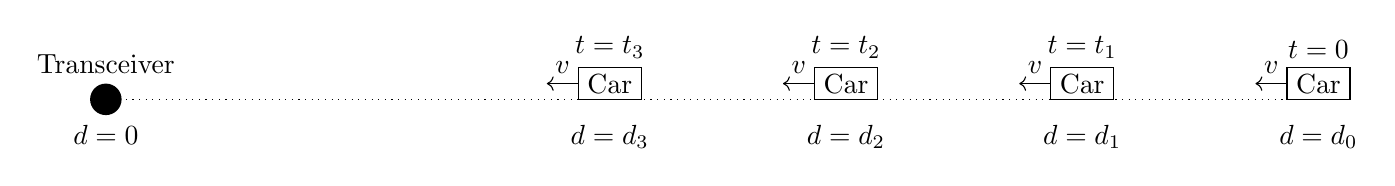
\begin{tikzpicture}

    % Draw the transceiver
    \fill[black] (0,0) circle (0.2) node[above] at (0,0.2) {Transceiver} node[below] at (0,-0.2) {$d=0$};

    % Draw the car at distance D_0
    \draw (15,0) rectangle ++(0.8,0.4) node[midway] {Car} node[above] at (15.4,0.4) {$t=0$ } node[below] at (15.4,-0.2) {$d=d_0$};
    \draw[->] (15,0.2) -- node[above] {$v$} (14.6,0.2);

    \draw (12,0) rectangle ++(0.8,0.4) node[midway] {Car} node[above] at (12.4,0.4) {$t=t_1$ } node[below] at (12.4,-0.2) {$d=d_1$};
    \draw[->] (12,0.2) -- node[above] {$v$} (11.6,0.2);

    \draw (9,0) rectangle ++(0.8,0.4) node[midway] {Car} node[above] at (9.4,0.4) {$t=t_2$ } node[below] at (9.4,-0.2) {$d=d_2$};
    \draw[->] (9,0.2) -- node[above] {$v$} (8.6,0.2);

    \draw (6,0) rectangle ++(0.8,0.4) node[midway] {Car} node[above] at (6.4,0.4) {$t=t_3$ } node[below] at (6.4,-0.2) {$d=d_3$};
    \draw[->] (6,0.2) -- node[above] {$v$} (5.6,0.2);

    \draw[dotted] (0,0) -- (15,0);

\end{tikzpicture}




  \caption{block diagram of the system}
  \label{fig:Gate2022_IN_39_f1}
\end{figure}

\begin{table}[!ht]
    \centering
        \begin{tabular}{|c|c|c|}
    \hline
    \textbf{Variable} & \textbf{Description} & \textbf{Value} \\
    \hline
    $v_c$ & velocity of laser & $3 \times 10^{8} \, \text{m/s}$ \\
    \hline
    $v$ & average speed of car & none \\
    \hline
    $t_1$ & time at which first pulse hits car & none \\
    \hline
     $t_2$ & time at which second pulse is emmited & $0.1\text{s}$ \\
    \hline
     $t_3$ & time at which  second pulse hits car & none \\
    \hline
    $d_0$  & Distance between tranceiver and car at $t=0$ & none \\
    \hline
    $d_i$ for $i=1,2,3$ & Distance between tranceiver and car at $t=t_i$ & none \\
    \hline
  \end{tabular}


    \caption{Input parameters}
    \label{tab:Gate2022_IN_39_t1}
\end{table}

From ~\figref{fig:Gate2022_IN_39_f1}
\begin{align}
    t_1&=\frac{d_1}{v_c}=\frac{d_0-d_1}{v}\\
\implies d_1&=\frac{d_0}{\left(1+\frac{v}{v_c}\right)}
\end{align}
Distance travelled by first pulse is given by 
\begin{align}
    2d_1 &= v_c \times 100 \, \text{ns}\\
    2\frac{d_0}{\left(1+\frac{v}{v_c}\right)}&=v_c \times 100 \, \text{ns}
    \label{eq:Gate2022_IN.39.4}
\end{align}
similarly time taken by car to move from $d_2$ to $d_3$ is given by
\begin{align}
    t_3-t_2&=\frac{d_3}{v_c}=\frac{d_2-d_3}{v}\\
    \implies d_3&=\frac{d_2}{\left(1+\frac{v}{v_c}\right)}
\end{align}
from ~\figref{fig:Gate2022_IN_39_f1}
\begin{align}
    d_2&=d_0-0.1v\\
\therefore d_3&=\frac{d_0-0.1v}{\left(1+\frac{v}{v_c}\right)}
\end{align}
Distance travelled by second pulse is given by 
\begin{align}
    2d_3 &= v_c \times 90 \, \text{ns}\\
    2\frac{d_0-0.1v}{\left(1+\frac{v}{v_c}\right)}&= v_c \times 90 \, \text{ns} \label{eq:Gate2022_IN.39.10}
\end{align}
solving ~\eqref{eq:Gate2022_IN.39.4} and ~\eqref{eq:Gate2022_IN.39.10} we get

\begin{align}
    v &= 15\, \text{m/s} \\
    v &=54\, \text{kmph}
\end{align}
since $v$ is same but time taken by pulses to reach tranceiver is decreasing, $v$ is towards tranceiver.\\
$\therefore$ Average speed of car is $54\,\text{kmph}$, moving towards the transceiver (option A )
%\end{document}

\item A rigid uniform annular disc is pivoted on a knife edge A in a uniform gravitational
field as shown, such that it can execute small amplitude simple harmonic motion in
the plane of the figure without slip at the pivot point. The inner radius $r$ and outer
radius $R$ are such that $r^2 = \frac{R^2}{2}$, and the acceleration due to gravity is $g$. If the
time period of small amplitude simple harmonic motion is given by $T = \beta \pi \sqrt{\frac{R}{g}}$,
where $\pi$ is the ratio of circumference to diameter of a circle, then $\beta$ =  (Round off to 2 decimal places)
\begin{figure}[h]
    %\caption{Stem Plot of $x(n)$ v/s n}
    \includegraphics[width=0.4\textwidth]{2022/ME/32/figs/11027_GATE_ME_32.png}\label{11027_GATE_ME_32}
    \caption{Question Diagram}
\end{figure}
\hfill{GATE 2022 ME-32}
\\
\solution
\iffalse
\let\negmedspace\undefined
\let\negthickspace\undefined
\documentclass[journal,12pt,twocolumn]{IEEEtran}
\usepackage{cite}
\usepackage{amsmath,amssymb,amsfonts,amsthm}
\usepackage{algorithmic}
\usepackage{graphicx}
\usepackage{textcomp}
\usepackage{xcolor}
\usepackage{txfonts}
\usepackage{listings}
\usepackage{enumitem}
\usepackage{mathtools}
\usepackage{gensymb}
\usepackage{comment}
\usepackage[breaklinks=true]{hyperref}
\usepackage{tkz-euclide} 
\usepackage{listings}
\usepackage{gvv}                                        
\def\inputGnumericTable{}                                 
\usepackage[latin1]{inputenc}                                
\usepackage{color}                                            
\usepackage{array}                                            
\usepackage{longtable}                                       
\usepackage{calc}                                             
\usepackage{multirow}                                         
\usepackage{hhline}                                           
\usepackage{ifthen}                                           
\usepackage{lscape}

\newtheorem{theorem}{Theorem}[section]
\newtheorem{problem}{Problem}
\newtheorem{proposition}{Proposition}[section]
\newtheorem{lemma}{Lemma}[section]
\newtheorem{corollary}[theorem]{Corollary}
\newtheorem{example}{Example}[section]
\newtheorem{definition}[problem]{Definition}
\newcommand{\BEQA}{\begin{eqnarray}}
\newcommand{\EEQA}{\end{eqnarray}}
\newcommand{\define}{\stackrel{\triangle}{=}}
\theoremstyle{remark}
\newtheorem{rem}{Remark}
\begin{document}
\bibliographystyle{IEEEtran}
\vspace{3cm}
\title{GATE 2022 ME-32}
\author{EE23BTECH11027 - K RAHUL$^{*}$% <-this % stops a space
}
\maketitle
\newpage
\bigskip
\renewcommand{\thefigure}{\theenumi}
\renewcommand{\thetable}{\theenumi}
\textbf{Question:}\\
A rigid uniform annular disc is pivoted on a knife edge A in a uniform gravitational
field as shown, such that it can execute small amplitude simple harmonic motion in
the plane of the figure without slip at the pivot point. The inner radius $r$ and outer
radius $R$ are such that $r^2 = \frac{R^2}{2}$, and the acceleration due to gravity is $g$. If the
time period of small amplitude simple harmonic motion is given by $T = \beta \pi \sqrt{\frac{R}{g}}$,
where $\pi$ is the ratio of circumference to diameter of a circle, then $\beta$ =  (Round off to 2 decimal places)
\begin{figure}[h]
    %\caption{Stem Plot of $x(n)$ v/s n}
    \includegraphics[width=0.4\textwidth]{2022/ME/32/figs/11027_GATE_ME_32.png}\label{11027_GATE_ME_32}
    \caption{Question Diagram}
\end{figure}
\hfill{GATE 2022 ME-32}
\\
\bigskip \bigskip


\solution
\fi
\begin{table}[ht]
\setlength{\arrayrulewidth}{0.3mm}
\setlength{\tabcolsep}{15pt}
\renewcommand{\arraystretch}{1.5}



\begin{tabular}{ |p{0.5 cm}|p{ 4cm}|p{1cm}| }
\hline
\multicolumn{3}{|c|}{Parameters in expression}\\
\hline
Symbol & Description & Value\\
\hline
$I$ & Moment of Inertia about the pivot point& $\frac{5}{4}MR^2$\\
\hline
$\theta \brak{t}$ & Angular displacement from vertical & ?\\
\hline
$\theta \brak{0}$ & Value of $\theta\brak{t}$ at $t=0$ & 0\\
\hline
$\Theta \brak{s}$ & Laplace Transform of $\theta \brak{t}$ & ?\\
\hline
$r$ & Distance of center of gravity from pivot point & $\frac{R}{\sqrt{2}}$\\
\hline
\end{tabular}
\caption{Parameters}
 %Table 1: Parameters



\end{table}


Moment of inertia of disc about pivot point is calculated as
\begin{align}
	I &= \frac{1}{2}\brak{R^2 + \frac{R^2}{2}} + \frac{MR^2}{2} \\
	&= \frac{5}{4}MR^2 \label{11027_Moment_Of_Inertia}
\end{align}

Using D' Alambert's principle,
\begin{align}
	&I\frac{d^2\theta \brak{t}}{dt^2} + mgr\sin\brak{\theta \brak{t}} = 0\\
	\implies& I\frac{d^2\theta \brak{t}}{dt^2} + mgr\theta \brak{t}= 0,\text{for } \theta \ll 1, \theta > 0 \label{11027_dAlambert_principle}
\end{align}

Using \eqref{11027_Moment_Of_Inertia} and \eqref{11027_dAlambert_principle}, we get
\begin{align}
	\frac{5MR^2}{4}&\frac{d^2 \theta \brak{t}}{dt^2} + Mg\frac{R}{\sqrt{2}} \theta \brak{t} = 0\\
	&\frac{d^2 \theta \brak{t}}{dt^2} + \frac{2\sqrt{2}g}{5R} \theta \brak{t}= 0 	
\end{align}
\\
Taking Laplace Transform on both sides,we get
\begin{align}
	s^2\Theta \brak{s} &- s \theta \brak{0} - \theta ' \brak{0} + \frac{2\sqrt{2}g}{5R} \Theta\brak{s}= 0\\
	\Theta\brak{s}&\brak{s^2+\frac{2\sqrt{2}g}{5R}} = \theta ' \brak{0}\\
	\Theta\brak{s}&= \frac{\theta ' \brak{0}}{\brak{s^2 + \frac{2\sqrt{2}g}{5R}}} \label{11027_alpha_s}
\end{align}
\\
\begin{align}
	u\brak{t}&\system{L}\frac{1}{s}\\
	e^{at}u\brak{t}&\system{L}\frac{1}{s-a}\\
	\frac{\brak{e^{jat} - e^{-jat}}}{2}u\brak{t}&\system \frac{a}{s^2+a^2}\\
	\sin\brak{at}&\system\frac{a}{s^2+a^2} \label{11027_Laplace_of_sine}
\end{align}
From \eqref{11027_alpha_s}
\begin{align}
	\Theta\brak{s}&= \frac{\theta ' \brak{0} \brak{\sqrt{\frac{2\sqrt{2}g}{5R} }} }{\brak{s^2 + \frac{2\sqrt{2}g}{5R}}} \frac{1}{ \brak{\sqrt{\frac{2\sqrt{2}g}{5R} }} }
\end{align}
\\
Taking inverse Laplace by putting $\frac{\theta ' \brak{0}}{\brak{\sqrt{\frac{2\sqrt{2}g}{5R}}}} = k$ and \eqref{11027_Laplace_of_sine}, 
\begin{align}
	\theta \brak{t} &= k \sin\brak{\frac{2\sqrt{2}g}{5R} t}\\
	T &= \frac{2 \pi}{\frac{2\sqrt{2}g}{5R}}\\
	&= \sqrt{\brak{5\sqrt{2}}}\:\pi \sqrt{\frac{R}{g}}
\end{align}
Thus, 
\begin{align}
	\beta = \sqrt{\brak{5\sqrt{2}}}\\
	\beta = 2.66
\end{align}
\begin{figure}[h]
    %\caption{Stem Plot of $x(n)$ v/s n}
    \includegraphics[width=0.4\textwidth]{2022/ME/32/figs/theta_t_plot.png}\label{11027_GATE_ME_32_thetaplot}
    \caption{Plot of $\theta\brak{t}$ for $(\theta'\brak{0}$, R) $\in$ \{(1,1) , (2,2) , (3,3)\}}
\end{figure}


\end{enumerate}

\section{2021}
\begin{enumerate}[label=\thechapter.\arabic*,ref=\thechapter.\theenumi]
\item A two degree of freedom spring-mass system undergoing free vibration
with generalized coordinates $ x_1$ and $ x_2$ has natural frequencies $ \omega_1=233.9\text{ rad/s}$ and $ \omega_2 = 324.5\text{ rad/s}$ , respectively. The corresponding mode shapes $ \phi_1=\begin{bmatrix}
1\\
-3.16
\end{bmatrix}$ and $ \phi_2=\begin{bmatrix}
1\\
3.16\end{bmatrix}$. If the system is disturbed with certain
deflections and zero initial velocities, then which of the following
statement(s) is/are true?


\begin{enumerate}
    \item[(A)] An initial deflection of $ x_1\brak{0}=6.32$cm and $ x_2\brak{0}=-3.16$cm would make the system oscillate with only the second natural frequency.
    \item[(B)]An initial deflection of $ x_1\brak{0}=2$cm and $ x_2\brak{0}=-6.32$cm would make the system oscillate with only the first natural frequency.
    \item[(C)] An initial deflection of $ x_1\brak{0}=2$cm and $ x_2\brak{0}=-2$cm would make the system oscillate with linear combination of first and second natural frequency.
    \item[(D)] An initial deflection of $ x_1\brak{0}=1$cm and $ x_2\brak{0}=-6.32$cm would make the system oscillate with only the first natural frequency.
\end{enumerate}
\hfill(GATE AE 2021 QUESTION 32)\\
\solution
\input{2021/AE/32/asnmt9.tex}
\pagebreak
\end{enumerate}

\chapter{Filters}
\section{2022}
\begin{enumerate}[label=\thechapter.\arabic*,ref=\thechapter.\theenumi]
\item The network shown below has a resonant frequency of 150 kHz and bandwidth of 600
Hz. The Q-factor of the network is \rule{1cm}{0.15mm}\\
(rounded off to one decimal place).\\
\hfill(GATE 2022 EC)\\
\begin{figure}[ht]
  \centering
  
      \begin{circuitikz}[american]
   \draw (0,8) to [sV=200V](0,-1) to [short](6,-1) to [short](6,0) to [D,l=$D_3$](9,3);
   \draw (0,8) to [short](6,8) to [short](6,6);
   \draw (6,6) to [D,l=$D_1$](9,3);
   \draw (3,3) to [D,l=$D_4$](6,6);
   \draw (3,3) to [D,l=$D_2$](6,0);
   \draw (3,3) to [short](2.5,3) to [crossing, bipoles/crossing/size=1](2.5,-4.8) to [short](12,-4.8) to [R=50$\Omega$](12,3) to [short](9,3);
   \draw (9,3) to [short,i=\Large{I}](12,3);
\end{circuitikz}

  
  \caption{Circuit 1}
\end{figure}\\
\solution\\
 \iffalse
\let\negmedspace\undefined
\let\negthickspace\undefined
\documentclass[journal,12pt,onecolumn]{IEEEtran}
\usepackage{cite}
\usepackage{amsmath,amssymb,amsfonts,amsthm}
\usepackage{algorithmic}
\usepackage{graphicx}
\usepackage{textcomp}
\usepackage{xcolor}
\usepackage{txfonts}
\usepackage{listings}
\usepackage{enumitem}
\usepackage{mathtools}
\usepackage{gensymb}
\usepackage{comment}
\usepackage[breaklinks=true]{hyperref}
\usepackage{tkz-euclide} 
\usepackage{tikz}
\usepackage{circuitikz}
%\usetikzlibrary{circuits.ee.IEC}
\usepackage{listings}
\usepackage{gvv} 
\usepackage{caption}
\def\inputGnumericTable{}                   

%\usepackage[latin1]{inputenc}                                
\usepackage{color}                                            
\usepackage{array}                                            
\usepackage{longtable}                                       
\usepackage{calc}                                             
\usepackage{multirow}                                         
\usepackage{hhline}                                           
\usepackage{ifthen}                                           
\usepackage{lscape}
\usepackage{tikz}
\usepackage{circuitikz}

\newtheorem{theorem}{Theorem}[section]
\newtheorem{problem}{Problem}
\newtheorem{proposition}{Proposition}[section]
\newtheorem{lemma}{Lemma}[section]
\newtheorem{corollary}[theorem]{Corollary}
\newtheorem{example}{Example}[section]
\newtheorem{definition}[problem]{Definition}
\newcommand{\BEQA}{\begin{eqnarray}}
\newcommand{\EEQA}{\end{eqnarray}}
\newcommand{\define}{\stackrel{\triangle}{=}}
\theoremstyle{remark}
\newtheorem{rem}{Remark}

\begin{document}

\bibliographystyle{IEEEtran}
\vspace{3cm}

\title{GATE: EE - 59.2022}
\author{EE23BTECH11013 - Avyaaz$^{*}$% <-this % stops a space 
}
\maketitle
% \newpage
% \bigskip

\renewcommand{\thefigure}{\arabic{figure}}
\renewcommand{\thetable}{\arabic{table}}

\large\textbf{\textsl{Question:}}
For the ideal AC-DC rectifier circuit shown in the figure below, the load current
magnitude is $I_{dc}$ = $15$ A and is ripple free. The thyristors are fired with a delay angle
of 45\degree
. The amplitude of the fundamental component of the source current, in
amperes, is \_\_\_\_\_\_\_\_{\em (Round off to 2
decimal places)}. \hfill(GATE 59 EE 2022)
\begin{figure}[!h]
\centering
\begin{circuitikz}[american voltages]
    \draw (0,0) node[op amp] (opamp) {};
    \draw (opamp.+) node[above]{$v_{+}$} to (-2,-0.5);
    \draw (opamp.-) node[above]{$v_{-}$} to (-2, 0.5);
    \draw (opamp.out) to (2, 0)node[right]{$v_{out}$};
    \draw (opamp.down) to (-0.1, -1) node[below]{$-v_{EE}$};
    \draw (opamp.up) to (-0.1, 1)node[above]{$+v_{DD}$};
    \draw (-2,0.5) to [R, l_=$R_1$](-3,0.5) to (-3.5, 0.5) to [V, l_=$0.1v$] (-3.5, -2) node[ground]{};
    \draw (-2, -0.5) to [R, l=$R_2$] (-2, -2) node[ground]{};
    \draw (-1.5,0.5) to (-1.5, 2) to [C, l=$C_1$] (1.5, 2) to (1.5, 0);
\end{circuitikz}

\end{figure}

\solution
\fi
\begin{table}[htbp]
\setlength{\extrarowheight}{4pt}
\setlength{\tabcolsep}{3pt}
\centering
\begin{tabular}{|c|c|c|}
\hline
\textbf{Parameter} & \textbf{Description}&\textbf{Value}\\
\hline 
$I_{dc}$& Load current & $15$A  \\
\hline
$\alpha$ &Firing angle&$45\degree$ \\
\hline
\end{tabular}

\caption{}
\label{tab:inputs.EE.59.2022}
\end{table}
% It is a Single phase symmetrical semi-converter.
% \begin{enumerate}[label={\roman*)}]
%     \item Load current magnitude $\brak{I_{dc}}$ = $15$A
%     \item Firing angle $\brak{\alpha} = 45\degree$
% \end{enumerate}
A symmetrical single phase semi converter is shown below,

\begin{figure}[!h]
\centering
    \begin{circuitikz}[scale = 0.8]
      \draw (-0.8,0.8) -- (-0.8,0.8) node[above]{$+$};
    \draw (0,2) to[sV,l=$V_s$] (0,-1);
     \draw (-0.8,0) -- (-0.8,0) node[below]{$-$};
    \draw (0,2) -- (2,2);
    \draw (2,2) -- (2,1);
    \draw (2,1) -- (3,1);
     \draw (3,1) to [thyristor] (3,3);
     \node at (2.4,2.3) {$T_1$};
    \draw (3,3) -- (5,3);
    \draw (5,1) to [thyristor] (5,3);
     \node at (4.4,2.3) {$T_2$};
    \draw (5,3) -- (7,3);
    \draw (7,3) to[resistor](7,1);
    \draw (7,1) -- (7,0);
    \draw(7,0) to [L](7,-2);
    \draw (7,-2) -- (3,-2);

    \draw (0, -1) -- (2,-1);
    \draw (2,-1) -- (2,0.4);
    \draw (2,0.4) -- (5,0.4);
    \draw (3,-2) to [Do] (3,0.4);
    \node at (3.8,-1) {$D_1$};
    \draw (3,0.4) -- (3,1);
    \draw (5,-2) to [Do] (5,0.4);
    \node at (5.8,-1) {$D_2$};
    \draw (5,0.4) -- (5,1);

     \draw[->] (6.5, 2) -- (6.5, 1) node[midway, left]{$I_{dc}$};
          \draw[->] (0.5, 2) -- (1, 2) ;
          \node at (1,1.6) {$I_s$};
          \node at (7.4,2) {$R$};
          \node at (7.4,-1.1) {$L$};

     \draw (8,2.8) -- (8,2.8) node[above]{$+$};
     \draw[->] (8,0.8) -- (8,2.8);
     \node at (8,0.5) {$V_o$};
     \draw[->] (8,0.2) -- (8,-1.8);
     \draw (8,-1.8) -- (8,-1.8) node[below]{$-$};
        \end{circuitikz}

\end{figure}

The Fourier series representation of supply current is given by:
\begin{align}
    i_s(t) = a_o +\sum_{n=1}^{\infty}C_n\sin({n\omega t} + \theta_n)\label{eq:gen_i_s}
\end{align}
 where,
 \begin{align}
 a_o &= \frac{1}{2\pi} \int_{0}^{2\pi} i_s(t)d\omega t \\
     C_n &= \sqrt{a_n^2 + b_n ^2}\label{eq:bino_coeff}\\
     \theta_n &= \tan^{-1}\left({\frac{a_n}{b_n}}\right)\label{eq: theta}
 \end{align}
\begin{align}
  \implies  a_o &= \frac{1}{2\pi}\int_{\alpha}^{\pi} I_o d\omega t - \int_{\pi + \alpha}^{2\pi} I_o d\omega t = 0\\
 \implies   a_n &= \frac{1}{\pi} \int_{\alpha}^{\pi}I_o\cos n\omega t d\omega t - \int_{\pi + \alpha}^{2\pi} I_o\cos{n\omega td\omega t}\\
 a_n &= 
 \begin{cases}
    \frac{-2I_o}{n\pi}\sin{n\alpha} & \text{for } n = 1,3,5...\\
     0 &\text{for } n = 2,4.....
    \end{cases}\\
 \implies   b_n &= \frac{1}{\pi}\int_{\alpha}^{\pi}I_o\sin n\omega t d\omega t - \int_{\pi + \alpha}^{2\pi} I_o\sin{n\omega td\omega t} \\
 b_n &= 
 \begin{cases}
     \frac{2I_o}{n\pi}\left(1 + \cos{n\alpha}\right) &\text{for } n = 1,3,5...\\
     0 &\text{for } n = 2, 4....
    \end{cases}
    \end{align}
From \eqref{eq:bino_coeff}:
\begin{align}
  \therefore  C_n &= \frac{2\sqrt{2}I_o}{n\pi}\left(\sqrt{1 + \cos{n\alpha}}\right)\\
  \implies  C_n &= \frac{4I_o}{n\pi}\cos{\frac{n\alpha}{2}}\label{eq:final_bino}
\end{align}
From \eqref{eq: theta}:
\begin{align}
    \theta_n &= \tan^{-1}\left(\frac{-\sin{n\alpha}}{1 + \cos{n\alpha}}\right)\\
    \implies \theta_n &= \frac{-n\alpha}{2}\label{eq:final_theta}
\end{align}

From \eqref{eq:gen_i_s},\eqref{eq:final_bino} and \eqref{eq:final_theta}:
\begin{align}
I_{s}(t) = \sum_{n=1,3,5...}^{\infty} \frac{4I_{o}}{n\pi}\cos{\frac{n\alpha}{2}}\sin{\left(n\omega t - \frac{n\alpha}{2}\right)}
\end{align}
% \begin{align}
% I_{s}(t) = \sum_{n=1,3,5...}^{\infty} \frac{4I_{dc}}{n\pi}\cos{\frac{n\alpha}{2}}\sin{\left(n\omega t - \frac{n\alpha}{2}\right)}
% \end{align}


% \begin{tikzpicture}[scale=1]
%     \draw[->] (0,0) -- (10,0) node[right] {$\omega t$};
%     \draw[->] (0,-2) -- (0,2) node[above] {$y$};
%     \draw[domain=0:10, smooth, variable=\x, black] plot ({\x},{sin(deg(\x))});
%     \foreach \x/\xtext in {1.57/\frac{\pi}{2},3.14/\pi,4.71/\frac{3\pi}{2},6.28/2\pi,7.85/\frac{7\pi}{2}} {
%         \draw (\x cm,0) -- (\x cm,0.1) node[below] {$\xtext$};
%     }
%     \foreach \y in {-1,1} {
%         \draw (1pt,\y cm-1.5) -- (-1pt,\y cm-1.5) node[left] {$\y$};
%     }
% \end{tikzpicture}

\begin{figure}[!h]
    \centering
    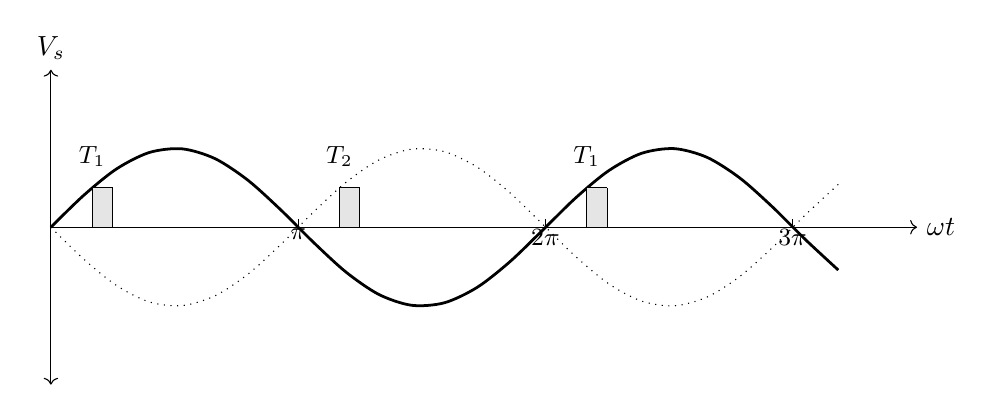
\begin{tikzpicture}[scale=1]
    \draw[->] (0,0) -- (11,0) node[right] {$\omega t$};
    \draw[<->] (0,-2) -- (0,2) node[above] {$V_s$};
    \draw[domain=0:10, smooth, variable=\x, black,line width=1pt] plot ({\x},{sin(deg(\x))});
    \draw[dotted,domain=0:10, smooth, variable=\x, black] plot ({\x},{-sin(deg(\x))});
    \foreach \x/\xtext in {3.14/\pi,6.28/2\pi,9.42/3\pi} {
        \draw (\x cm,0) -- (\x cm,0.1) node[below] {\small$\xtext$};
    }

\fill[gray!20] (0.5233,0) -- (0.5233,0.5) -- (0.785,0.5) -- (0.785,0) -- cycle;
    \fill[gray!20] (3.6633,0) -- (3.6633,0.5) -- (3.925,0.5) -- (3.925,0) -- cycle;
    \fill[gray!20] (6.8033,0) -- (6.8033,0.5) -- (7.065,0.5) -- (7.065,0) -- cycle;

    \draw (0.5233,0) -- (0.5233,0.5);
    \draw (0.5233,0.5) -- (0.785,0.5);
    \draw (0.785,0.5) -- (0.785,0);

    \draw (3.6633,0) -- (3.6633,0.5);
    \draw (3.6633,0.5) -- (3.925,0.5);
    \draw (3.925,0.5) -- (3.925,0);

    \draw (6.8033,0) -- (6.8033,0.5);
    \draw (6.8033,0.5) -- (7.065,0.5);
    \draw (7.065,0.5) -- (7.065,0);


     \node at (0.5233,0.9) {\small$T_1$};
     \node at (3.6633,0.9) {\small$T_2$};
     \node at (6.8033,0.9) {\small$T_1$};
\end{tikzpicture}
\end{figure}
\begin{figure}[!h]
    \centering
    \begin{tikzpicture}[scale=1]
    \draw[->] (0,0) -- (11,0) node[right] {$\omega t$};
    \draw[<->] (0,-2) -- (0,2) node[above] {$V_o$};
    \draw[domain=0.5233:3.14, smooth, variable=\x, black,line width=1pt] plot ({\x},{sin(deg(\x))});
    \draw[domain=3.6633:6.28, smooth, variable=\x, black,line width=1pt] plot ({\x},{-sin(deg(\x))});
    \draw[domain=6.8033:9.42, smooth, variable=\x, black,line width=1pt] plot ({\x},{sin(deg(\x))});

    \foreach \x/\xtext in {0.5233/\alpha, 3.14/\pi,4/\pi + \alpha ,6.28/2\pi,7.2/2\pi + \alpha,9.42/3\pi}{
        \draw (\x cm,0) -- (\x cm,0) node[below] {\small $\xtext$};
    }

     \draw [line width=1pt](0,0)--(0.5233,0);
    \draw [line width=1pt](0.5233,0) -- (0.5233,0.5);
    \draw[line width=1pt](3.14,0)-- (3.6633,0);
    \draw[line width=1pt] (3.6633,0) -- (3.6633,0.5);
    \draw [line width=1pt](6.28,0)--(6.8033,0);
    \draw [line width=1pt](6.8033,0) -- (6.8033,0.5);

    \node at (0.25,0.6){\small$T_2$};
    \node at (0.25,0.2){\small$D_2$};
     \node at (3.4,0.6){\small$T_1$};
    \node at (3.4,0.2){\small$D_1$};
    \node at (6.4,0.6){\small$T_2$};
    \node at (6.4,0.2){\small$D_2$};

    \node at (1.57,0.4){\small $T_1D_2$};
    \node at (4.71,0.4){\small $T_2D_1$};
    
\end{tikzpicture}
\end{figure}
\begin{figure}[!h]
    \centering
    \begin{tikzpicture}[scale=1]
    \draw[->] (0,0) -- (11,0) node[right] {$\omega t$};
    \draw[<->] (0,-2) -- (0,2) node[above] {$i_{T_1}$};
   
    \foreach \x/\xtext in {0.5233/\alpha,4/\pi + \alpha,7.2/2\pi + \alpha,10/3\pi + \alpha}{
        \draw (\x cm,0) -- (\x cm,0) node[below] {\small $\xtext$};
    }
     \draw [line width=1pt](0,0)--(0.5233,0);
    \draw [line width=1pt](0.5233,0) -- (0.5233,1);
    \draw[line width=1pt](0.5233,1)-- (3.6633,1);
    \draw[line width=1pt] (3.6633,1) -- (3.6633,0);
    \draw[line width=1pt] (3.6633,0) -- (6.8033,0);
    \draw [line width=1pt](6.8033,0)--(6.8033,1);
    \draw [line width=1pt](6.8033,1) -- (9.948,1);
     \draw [line width=1pt] (9.948,1) -- (9.948,0);

     \draw[dotted,domain=0:10, smooth, variable=\x, black] plot ({\x},{1});
     \node at (0.4,1.2) {\small $I_{DC}$};
\end{tikzpicture}
\end{figure}
\begin{figure}[!h]
    \centering
    \begin{tikzpicture}[scale=1]
    \draw[->] (0,0) -- (11,0) node[right] {$\omega t$};
    \draw[<->] (0,-2) -- (0,2) node[above] {$i_{s}$};
   

    \draw [line width=1pt](0.5233,0) -- (0.5233,1);
    \draw[line width=1pt](0.5233,1)-- (3.14,1);
    \draw[line width=1pt](3.14,1)-- (3.14,0);
    \draw[line width=1pt] (3.14,0) -- (3.6633,0);
    \draw[line width=1pt] (3.6633,0) -- (3.6633,-1);
    \draw[line width=1pt] (3.6633,-1) -- (6.28,-1);
    \draw[line width=1pt]  (6.28,-1) -- (6.28,0);
    \draw[line width=1pt] (6.28,0) -- (6.8033,0);
    \draw [line width=1pt](6.8033,0)--(6.8033,1);
    \draw [line width=1pt](6.8033,1) -- (9.42,1);
     \draw [line width=1pt] (9.42,1) -- (9.42,0);
     \draw [line width=1pt] (9.42,0) -- (9.948,0);

     \draw[dotted,domain=0:10, smooth, variable=\x, black] plot ({\x},{1});
     \node at (0.4,1.2) {\small $I_{DC}$};
    
\end{tikzpicture}
\end{figure}

From \tabref{tab:inputs.EE.59.2022}:
\begin{align}
   (I_{s_1})_{peak} &= \frac{4I_{dc}}{\pi}\cos{\left(\frac{\alpha}{2}\right)}\\
    &= \frac{4 \times 15 }{\pi}\times \cos{\frac{45 \degree}{2}}\\
    &=17.64 A 
\end{align}

%\end{document}

\pagebreak

\item In the circuit shown below, the switch S is closed at $t=0$. The magnitude of the steady state voltage, in volts, across the $6\Omega$ resistor is \_\_\_\_\_.(\textit{round off to two decimal places})\\ \hfill(GATE 2022 EE Q31)
\begin{figure}[!h]
    \centering
    \begin{circuitikz}[scale = 0.8]
        \draw(0, 0) -- (1, 0);
        \draw(1, 0.5) -- (1, -0.5);
        \draw(4, 0.5) -- (4, -0.5);
        \draw(4, 0) -- (5, 0);

        \draw(1, 0.5) to[R, l = $6\Omega$](4, 0.5);
        \draw(1, -0.5) to[R, l_ = $3\Omega$](4, -0.5);

        \draw(0, 0) -- (0, -2);
        \draw(5, 0) -- (5, -2);

        \draw(0, -2) to[C, l = $1\mu F$](2, -2);
        \draw(2, -2) to [R, l = $10\Omega$](5, -2);

        \draw(0, -2) -- (0, -3.5);
        \draw(5, -2) -- (5, -3.5);

        \draw(0, -3.5) to[battery2, l_ = $10V$](1.5, -3.5);
        \draw (1.5, -3.5) to[switch, l = S] (2, -3.5);
        \draw(2, -3.5) to [R, l = $2\Omega$](5, -3.5);

        \draw[->](0, -3.5) -- (0, -2.5) node[midway, left] {$I$}; 
    \end{circuitikz}
    \caption{}
    \label{fig:1_gate.ee.22.31}
\end{figure}\\
\solution
		\iffalse
\let\negmedspace\undefined
\let\negthickspace\undefined
\documentclass[journal,12pt,twocolumn]{IEEEtran}
\usepackage{cite}
\usepackage{amsmath,amssymb,amsfonts,amsthm}
\usepackage{algorithmic}
\usepackage{graphicx}
\usepackage{textcomp}
\usepackage{xcolor}
\usepackage{txfonts}
\usepackage{listings}
\usepackage{enumitem}
\usepackage{mathtools}
\usepackage{gensymb}
\usepackage{comment}
\usepackage[breaklinks=true]{hyperref}
\usepackage{tkz-euclide} 
\usepackage{listings}
\usepackage{gvv}                            \usepackage{tikz}
\usepackage{circuitikz}
\def\inputGnumericTable{}                                
\usepackage[latin1]{inputenc}                            
\usepackage{color}                                       
\usepackage{array}                                       
\usepackage{longtable}                                   
\usepackage{calc}                              
\usepackage{tikz}
\usepackage{multirow}                                    
\usepackage{hhline}                                      
\usepackage{ifthen}                            
\usepackage{caption}
\usepackage{lscape}
\usepackage{amsmath}
\newtheorem{theorem}{Theorem}[section]
\newtheorem{problem}{Problem}
\newtheorem{proposition}{Proposition}[section]
\newtheorem{lemma}{Lemma}[section]
\newtheorem{corollary}[theorem]{Corollary}
\newtheorem{example}{Example}[section]
\newtheorem{definition}[problem]{Definition}
\newcommand{\BEQA}{\begin{eqnarray}}
\newcommand{\EEQA}{\end{eqnarray}}
\newcommand{\define}{\stackrel{\triangle}{=}}
\theoremstyle{remark}
\newtheorem{rem}{Remark}

\begin{document}

\bibliographystyle{IEEEtran}
\vspace{3cm}

\title{GATE 2023 PH Q37}
\author{EE23BTECH11009 - AROSHISH PRADHAN$^{*}$% <-this % stops a space
}
\maketitle
\newpage
\bigskip
\textbf{Question:} In the circuit shown below, the switch S is closed at $t=0$. The magnitude of the steady state voltage, in volts, across the $6\Omega$ resistor is \_\_\_\_\_.(\textit{round off to two decimal places})\\ \hfill(GATE 2022 EE Q31)
\begin{figure}[!h]
    \centering
    \begin{circuitikz}[scale = 0.8]
        \draw(0, 0) -- (1, 0);
        \draw(1, 0.5) -- (1, -0.5);
        \draw(4, 0.5) -- (4, -0.5);
        \draw(4, 0) -- (5, 0);

        \draw(1, 0.5) to[R, l = $6\Omega$](4, 0.5);
        \draw(1, -0.5) to[R, l_ = $3\Omega$](4, -0.5);

        \draw(0, 0) -- (0, -2);
        \draw(5, 0) -- (5, -2);

        \draw(0, -2) to[C, l = $1\mu F$](2, -2);
        \draw(2, -2) to [R, l = $10\Omega$](5, -2);

        \draw(0, -2) -- (0, -3.5);
        \draw(5, -2) -- (5, -3.5);

        \draw(0, -3.5) to[battery2, l_ = $10V$](1.5, -3.5);
        \draw (1.5, -3.5) to[switch, l = S] (2, -3.5);
        \draw(2, -3.5) to [R, l = $2\Omega$](5, -3.5);

        \draw[->](0, -3.5) -- (0, -2.5) node[midway, left] {$I$}; 
    \end{circuitikz}
    \caption{}
    \label{fig:1_gate.ee.22.31}
\end{figure}\\

\solution 
\fi
Consider a sinusoidal input source of angular frequency $\omega$.

\begin{table}[!h]
    \centering
    \begin{tabular}{|c|c|c|}
    \hline
       \textbf{Symbol}  &  \textbf{Value}  &  \textbf{Description}\\
    \hline
       $\omega$  &  $0$ for D.C. &  Angular Frequency\\
    \hline
        $C$ & $1\mu F$ & Capacitance \\
    \hline
        $V_{in}(t)$ & $10\cos(\omega t)$ & Input Voltage\\
    \hline
        $V_{out}(t)$ &  & Output Voltage across $6\Omega$\\
    \hline
        $V_{out}(j\omega)$ & $H(j\omega)V_{in}(j\omega)$ & Output in Frequency Domain\\
    \hline
        $H(j\omega)$ &  & Transfer Function\\
    \hline
        $I(j\omega)$ & & Total Current\\
    \hline
        $Z_{\text{eff}}$ & & Overall Impedance\\
    \hline
    \end{tabular}
    \caption{Given Parameters}
    \label{tab:1_gate.22.ee.31}
\end{table}

Using KCL and KVL, we can calculate:
\begin{align}
    Z_{\text{eff}} &= \frac{2\brak{10 + \frac{1}{j\omega C}}}{12 + \frac{1}{j\omega C}} + 2\\
    \implies I(j\omega) &= \frac{V_{in}}{\brak{\frac{2\brak{10 + \frac{1}{j\omega C}}}{12 + \frac{1}{j \omega C}}+2}}\\
    \implies V_{out}(j\omega) &= 2\sbrak{\brak{\frac{10 + \frac{1}{j\omega C}}{12 + \frac{1}{j\omega C}}}I(j\omega)}\\
    &= 2\sbrak{\brak{\frac{10 + \frac{1}{j\omega C}}{12 + \frac{1}{j\omega C}}}\frac{V_{in}(j\omega)}{\brak{\frac{2\brak{10 + \frac{1}{j\omega C}}}{12 + \frac{1}{j \omega C}}+2}}}\\
    \implies H(j\omega) &= \frac{1 + 10j\omega C}{2(1 + 11j\omega C)}
\end{align}
\begin{figure}[!h]
    \centering
    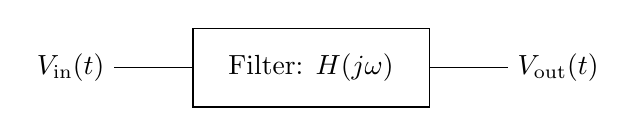
\begin{tikzpicture}
    % Draw the filter rectangle
    \draw (0,0) rectangle (3,1) node[midway] {Filter: $H(j\omega)$};
    
    % Draw the input and output labels
    \draw (-1,0.5) node[left] {$V_{\text{in}}(t)$} -- (0,0.5);
    \draw (3,0.5) -- (4,0.5) node[right] {$V_{\text{out}}(t)$};
\end{tikzpicture}
    \caption{Filter Equivalent of Circuit}
    \label{fig:2_gate.22.ee.31}
\end{figure}
\begin{align}
    H(j\omega) &= \brak{\frac{\sqrt{1 + 100\omega^2 C^2}}{2\sqrt{1 + 121\omega^2 C^2}}}e^{j(\tan^{-1}(10\omega C) - \tan^{-1}(11\omega C))}\\
    &= \brak{\frac{\sqrt{1 + 100\omega^2 C^2}}{2\sqrt{1 + 121\omega^2 C^2}}}e^{j\tan^{-1}\brak{\frac{-\omega C}{1 + 110\omega^2 C^2}}}\\
    \therefore V_{out}(t) &= 10\abs{H(j\omega)}\cos(\omega t + \angle H(j\omega))\\
    &= \frac{5\sqrt{1 + 100\omega^2 C^2}}{\sqrt{1 + 121\omega^2 C^2}}\cos\brak{\omega t -\tan^{-1}\brak{\frac{\omega C}{1 + 110\omega^2 C^2}}}
\end{align}
\begin{figure}[!h]
    \centering
    \includegraphics[width = \columnwidth]{2022/EE/31/figs/V_out_plot.png}
    \caption{Plot of $V_{out}(t)$ at $t=0$ w.r.t $\omega$}
    \label{fig:3_gate.22.ee.31}
\end{figure}

As $\omega \rightarrow 0$, $V_{in}(t)$ approaches being a D.C. input source ($10V$).

$\therefore$ substituting $\omega = 0$, we get:
\begin{align}
    V_{out}(t) &= 5V
\end{align}

%\end{document}


\pagebreak
\end{enumerate}

\section{2021}
\begin{enumerate}[label=\thechapter.\arabic*,ref=\thechapter.\theenumi]
\item A speech signal, band limited to 4 kHz, is sampled at 1.25 times the Nyquist rate. The speech samples, assumed to be statistically independent and uniformly distributed in the range -5 V to +5 V, are subsequently quantized in an 8-bit uniform quantizer and then over a voice-grade AWGN telephone channel. If the ratio of transmitted signal power to channel noise power is 26 dB, the minimum channel bandwidth required to ensure reliable transmission of the signal with arbitrarily small probability of transmission error (\textit{rounded off to one decimal place}) is \rule{1cm}{0.15mm} kHz.
\hfill (GATE EC 2021)
\solution
\iffalse
\let\negmedspace\undefined
\let\negthickspace\undefined
\documentclass[journal,12pt,twocolumn]{IEEEtran}
\usepackage{cite}
\usepackage{amsmath,amssymb,amsfonts,amsthm}
\usepackage{algorithmic}
\usepackage{graphicx}
\usepackage{textcomp}
\usepackage{xcolor}
\usepackage{txfonts}
\usepackage{listings}
\usepackage{enumitem}
\usepackage{mathtools}
\usepackage{gensymb}
\usepackage{comment}
\usepackage[breaklinks=true]{hyperref}
\usepackage{tkz-euclide}
\usepackage{listings}
\usepackage{gvv}
\def\inputGnumericTable{}
\usepackage[latin1]{inputenc}
\usepackage{color}
\usepackage{array}
\usepackage{longtable}
\usepackage{calc}
\usepackage{multirow}
\usepackage{hhline}
\usepackage{ifthen}
\usepackage{lscape}

\newtheorem{theorem}{Theorem}[section]
\newtheorem{problem}{Problem}
\newtheorem{proposition}{Proposition}[section]
\newtheorem{lemma}{Lemma}[section]
\newtheorem{corollary}[theorem]{Corollary}
\newtheorem{example}{Example}[section]
\newtheorem{definition}[problem]{Definition}
\newcommand{\BEQA}{\begin{eqnarray}}
\newcommand{\EEQA}{\end{eqnarray}}
\newcommand{\define}{\stackrel{\triangle}{=}}
\theoremstyle{remark}
\newtheorem{rem}{Remark}
\begin{document}

\bibliographystyle{IEEEtran}
\vspace{3cm}

\title{GATE 2021 EC 23}
\author{EE23BTECH11007 - Aneesh Kadiyala$^{*}$% <-this % stops a space
}
\maketitle
\newpage
\bigskip

\renewcommand{\thefigure}{\theenumi}
\renewcommand{\thetable}{\theenumi}

\vspace{3cm}
\textbf{Question:} A speech signal, band limited to 4 kHz, is sampled at 1.25 times the Nyquist rate. The speech samples, assumed to be statistically independent and uniformly distributed in the range -5 V to +5 V, are subsequently quantized in an 8-bit uniform quantizer and then over a voice-grade AWGN telephone channel. If the ratio of transmitted signal power to channel noise power is 26 dB, the minimum channel bandwidth required to ensure reliable transmission of the signal with arbitrarily small probability of transmission error (\textit{rounded off to one decimal place}) is \rule{1cm}{0.15mm} kHz.

\hfill(GATE 2021 EC)
\\
\solution
\\
\fi
\begin{table}[h!]
    \centering
    \begin{tabular}{ | c | c | c | }
    \hline
    Parameter & Value & Description \\
    \hline
    $B_0$ & 4 kHz & Bandwidth of signal \\
    \hline
    $R_N$ & $2B_0$ & Nyquist Rate \\
    \hline
    $f_s$ & $1.25R_N$ & Sampling Frequency \\
    \hline
    $R$ & $nf_s$ & Data Rate \\
    \hline
    $C$ & $B\log_2{\brak{1 + \frac{P}{N}}}$ & Capacity of AWGN \\
    & & Channel with bandwidth $B$ \\
    \hline
    $10\log_{10}{\frac{P}{N}}$ & 26 dB & Signal to Noise Ratio \\
    \hline
\end{tabular}
    \caption{Input Parameters}
    \label{tab:2021ec23_1}
\end{table}

The signal is band limited to 4 kHz.
\begin{align}
B_0 &= 4\text{kHz} \\
%R_N &= 2B_0 \\
\implies R_N &= 8\text{kHz} \\
%f_s &= 1.25R_N \\
\implies f_s &= 10\text{kHz} \\
%R &= nf_s \\
R &= \brak{8}\brak{10\text{kHz}} \\
\implies R &= \brak{8}\brak{10^4}\text{ bits/second}
\end{align}
Channel capacity for an Additive White Gaussian Noise channel is
\begin{align}
C = B\log_2{\brak{1 + \frac{P}{N}}}\text{ bits/second}
\end{align}
where $P$ is the maximum channel power and $N$ is the noise power and $B$ is the channel bandwidth.
\begin{align}
10\log_{10}{\frac{P}{N}} &= 26\text{dB} \\
\implies \frac{P}{N} &= 10^{2.6} \\
&\approx 398.107
\end{align}
For reliable transmission:
\begin{align}
R &\le C \\
8\brak{10^4} &\le B\log_2{399.107} \\
B &\ge \frac{8\brak{10^4}}{\log_2{399.107}} \\
\implies B &\ge 9258.58\text{Hz}
\end{align}
$\therefore$ the minimum channel bandwidth required to ensure reliable transmission of the signal is $\approx9.26$ kHz.
\pagebreak
\end{enumerate}

\chapter{ Z-transform}
\section{2022}
\begin{enumerate}[label=\thechapter.\arabic*,ref=\thechapter.\theenumi]

\item Consider the following recursive iteration scheme for different values of variable P with the initial guess $x_1=1$:
$$x_{n+1}=\frac{1}{2}\brak{x_n+\frac{P}{x_n}}, \quad\quad n=1,2,3,4,5 $$
For $P=2$, $x_5$ is obtained to be 1.414, rounded off to 3 decimal places. For $P=3$, $x_5$ is obtained to be 1.732, rounded off to 3 decimal places.   \\ \\
If $P=10$, the numerical value of $x_5$ is \rule{1.3cm}{0.15mm} . ($round$ $off$ $to$ $three$ $decimal$ $places$)     \hfill(GATE CE 2022) \\
\solution 
% \iffalse
\let\negmedspace\undefined
\let\negthickspace\undefined
\documentclass[journal,12pt,twocolumn]{IEEEtran}
\usepackage{cite}
\usepackage{amsmath,amssymb,amsfonts,amsthm}
\usepackage{algorithmic}
\usepackage{graphicx}
\usepackage{textcomp}
\usepackage{xcolor}
\usepackage{txfonts}
\usepackage{listings}
\usepackage{enumitem}
\usepackage{mathtools}
\usepackage{gensymb}
\usepackage{comment}
\usepackage[breaklinks=true]{hyperref}
\usepackage{tkz-euclide} 
\usepackage{listings}
\usepackage{gvv}                                        
\def\inputGnumericTable{}                                 
\usepackage[latin1]{inputenc}                                
\usepackage{color}                                            
\usepackage{array}                                            
\usepackage{longtable}                                       
\usepackage{calc}                                             
\usepackage{multirow}                                         
\usepackage{hhline}                                           
\usepackage{ifthen}                                           
\usepackage{lscape}

\newtheorem{theorem}{Theorem}[section]
\newtheorem{problem}{Problem}
\newtheorem{proposition}{Proposition}[section]
\newtheorem{lemma}{Lemma}[section]
\newtheorem{corollary}[theorem]{Corollary}
\newtheorem{example}{Example}[section]
\newtheorem{definition}[problem]{Definition}
\newcommand{\BEQA}{\begin{eqnarray}}
\newcommand{\EEQA}{\end{eqnarray}}
\newcommand{\define}{\stackrel{\triangle}{=}}
\theoremstyle{remark}
\newtheorem{rem}{Remark}
\begin{document}
\parindent 0px
\bibliographystyle{IEEEtran}
\title{GATE: CE - 29.2022}
\author{EE22BTECH11219 - Rada Sai Sujan$^{}$% <-this % stops a space
}
\maketitle
\newpage
\bigskip
\section*{Question}
Consider the following recursive iteration scheme for different values of variable P with the initial guess $x_1=1$:
$$x_{n+1}=\frac{1}{2}\brak{x_n+\frac{P}{x_n}}, \quad\quad n=1,2,3,4,5 $$
For $P=2$, $x_5$ is obtained to be 1.414, rounded off to 3 decimal places. For $P=3$, $x_5$ is obtained to be 1.732, rounded off to 3 decimal places.   \\ \\
If $P=10$, the numerical value of $x_5$ is \rule{1.3cm}{0.15mm} . ($round$ $off$ $to$ $three$ $decimal$ $places$)     \hfill(GATE CE 2022) \\
\solution 

Applying $A.M \geq G.M$ inequality,
\begin{align}
    \frac{x_n+\frac{P}{x_n}}{2} \geq \sqrt{P}   \\
    \implies x_{n+1} \geq \sqrt{P}  \label{eq:ce.29.22.1}
\end{align}
Solving the equation,
\begin{align}
    2x_{n+1}x_{n} - {x_n}^2 - P &=0
\end{align}
Applying $Z$-transform we get,
\begin{align}
    X\brak{z} \ast X\brak{z} &= \frac{PZ^{-1}}{\brak{1-z^{-1}}\brak{2-z^{-1}}}  \\
    &= P\brak{\frac{z^{-1}}{1-z^{-1}} - \frac{z^{-1}}{2-z^{-1}}}
\end{align}
From the transformation pairs,
\begin{align}
    x_{n-a} &\overset{\mathcal{Z}}{ \longleftrightarrow} z^{-a}X\brak{z}  \\
    x_{n_1}\times x_{n_2} &\overset{\mathcal{Z}}{ \longleftrightarrow} X_1\brak{z}\ast X_2\brak{z} \\
    \frac{u\brak{n-1}}{a^{n}} &\overset{\mathcal{Z}}{ \longleftrightarrow} \frac{z^{-1}}{a-z^{-1}}
\end{align}
Now, applying inverse $Z$-tranform,
\begin{align}
    x_n^2 &= P\brak{u\brak{n-1} - \frac{u\brak{n-1}}{2^n}}  \\
    \implies x_n^2 &=P\brak{1-\frac{1}{2^n}} \quad \text{[$\because n \geq 1$]}
\end{align}
Similarly,
\begin{align}
    x_{n+1}^2 &= P\brak{1 - \frac{1}{2^{n+1}}}  \\
    \implies \lim\limits_{n\to\infty}\frac{x_{n+1}}{x_n} &= \lim\limits_{n\to\infty}\sqrt{\frac{P\brak{1-\frac{1}{2^n}}}{P\brak{1-\frac{1}{2^{n+1}}}}}    \\
    &=1
\end{align}
Hence, the system is convergent.    \\
Now finding the limit of the sequence,
\begin{align}
    x^2 &=\lim\limits_{x\to\infty}P\brak{1-\frac{1}{2^n}}   \\
    \implies x &= \pm\sqrt{P}   \label{eq:ce.29.22.11}
\end{align}
From \eqref{eq:ce.29.22.1} and \eqref{eq:ce.29.22.11},
\begin{align}
    x_{n+1}=\sqrt{P}
\end{align}
Therefore, for $P=10$ the value of $x_5$ is,
\begin{align}
    x_5&=\sqrt{10}  \\
    \therefore x_5&=3.162
\end{align}
\end{document}

\newpage

\end{enumerate}

\section{2021}
\begin{enumerate}[label=\thechapter.\arabic*,ref=\thechapter.\theenumi]
\item The causal signal with Z transform $z^2(z - a)^{-2}$ is ($u(n)$ is unit step signal)
\begin{enumerate}
    \item $a^{2n}u(n)$
    \item $(n + 1)a^nu(n)$
    \item $n^{-1}a^nu(n)$
    \item $n^2a^nu(n)$
\end{enumerate}

\hfill(GATE 31 EE 2021) 

\solution
 \iffalse
\let\negmedspace\undefined
\let\negthickspace\undefined
\documentclass[journal,12pt,twocolumn]{IEEEtran}
\usepackage{cite}
\usepackage{amsmath,amssymb,amsfonts,amsthm}
\usepackage{algorithmic}
\usepackage{graphicx}
\usepackage{textcomp}
\usepackage{xcolor}
\usepackage{txfonts}
\usepackage{listings}
\usepackage{enumitem}
\usepackage{mathtools}
\usepackage{gensymb}
\usepackage{comment}
\usepackage[breaklinks=true]{hyperref}
\usepackage{tkz-euclide} 
\usepackage{tikz}
% \usetikzlibrary{positioning, arrows.meta}
\usepackage{listings}
\usepackage{gvv} 
\usepackage{caption}
\def\inputGnumericTable{}                   

%\usepackage[latin1]{inputenc}                                
\usepackage{color}                                            
\usepackage{array}                                            
\usepackage{longtable}                                       
\usepackage{calc}                                             
\usepackage{multirow}                                         
\usepackage{hhline}                                           
\usepackage{ifthen}                                           
\usepackage{lscape}
\usepackage{tikz}
\newtheorem{theorem}{Theorem}[section]
\newtheorem{problem}{Problem}
\newtheorem{proposition}{Proposition}[section]
\newtheorem{lemma}{Lemma}[section]
\newtheorem{corollary}[theorem]{Corollary}
\newtheorem{example}{Example}[section]
\newtheorem{definition}[problem]{Definition}
\newcommand{\BEQA}{\begin{eqnarray}}
\newcommand{\EEQA}{\end{eqnarray}}
\newcommand{\define}{\stackrel{\triangle}{=}}
\theoremstyle{remark}
\newtheorem{rem}{Remark}

\begin{document}

\bibliographystyle{IEEEtran}
\vspace{3cm}

\title{GATE: EE - 31.2021}
\author{EE23BTECH11013 - Avyaaz$^{*}$% <-this % stops a space 
}
\maketitle
\newpage
\bigskip

\renewcommand{\thefigure}{\arabic{figure}}
\renewcommand{\thetable}{\arabic{table}}

\large\textbf{\textsl{Question:}}
The causal signal with Z transform $z^2(z - a)^{-2}$ is ($u(n)$ is unit step signal)
\begin{enumerate}
    \item $a^{2n}u(n)$
    \item $(n + 1)a^nu(n)$
    \item $n^{-1}a^nu(n)$
    \item $n^2a^nu(n)$
\end{enumerate}

\hfill(GATE EE 2021) \\
\solution
\fi
% \begin{table}[htbp]
%     \centering
%      \begin{table}[!ht] 
\centering
\setlength{\extrarowheight}{8pt}
\begin{tabular}{|l|l|l|}
    \hline
    \textbf{Parameter} & \textbf{Description} & \textbf{Values}\\
    \hline
     m & load of system &  \\
    \hline
     k & stiffness of system &  \\
    \hline
     $\omega_n$ & Natural frequency & $\sqrt{\frac{k}{m}}$ \\
    \hline
    $\zeta$ & Damping ratio & $\frac{c}{2m\omega_n}$ \\
    \hline
     y\brak{t} & Output of system & \\
    \hline
     x\brak{t} & Input to the system & \\
    \hline
     c & Damping coefficient & \\
    \hline
    T\brak{s} & Transfer function of system & $\frac{Y\brak{s}}{R\brak{s}}$\\
    \hline
  \end{tabular}
  \vspace{4mm}
 \caption{Parameter Table}
 \label{tab:table0_ee_22_39}
\end{table}

%     \caption{}
%     \label{tab:my_label.41.IN.2022}
% \end{table}

% \begin{figure}[!htbp]
%     \resizebox{0.501\textwidth}{!}{\tikzset{
    block/.style = {draw, fill=white, rectangle, minimum height=3em, minimum width=3em},
    tmp/.style  = {coordinate}, 
    minus/.style= {draw, fill=white, circle, node distance=1cm, append after command={\pgfextra \draw ($(\tikzlastnode.center) + (-0.15,0)$) -- ($(\tikzlastnode.center) + (0.15,0)$) node[above] {$-$}; \endpgfextra}},
    plus/.style= {draw, fill=white, circle, node distance=1cm, append after command={\pgfextra \draw ($(\tikzlastnode.center) + (-0.15,0)$) -- ($(\tikzlastnode.center) + (0.15,0)$) node[above] {$+$}; \endpgfextra}},
    input/.style = {coordinate},
    output/.style= {coordinate},
    pinstyle/.style = {pin edge={to-,thin,black}}
}


\begin{tikzpicture}[auto, node distance=2cm]
    % Blocks
    \node [input, name=rinput] (rinput) at (0,0) {};
    \node [minus] (sum1) at (1,0) {};
    \node [block] (controller) at (3,0) {$K_{p}$};
    \node [block] (kd) at (3,-2) {$sK_D$};
    \node [block] (up) at (3,2) {\Large$\frac{K_{i}}{s}$};
    \node [plus] (sum2) at (5,0) {};
    \node [block] (system) at (7,0) {$P\brak{s}=\frac{1}{\brak{s+1}\brak{s+2}}$};
    \node [output] (output) at (9,0) {};
    \node [tmp] (tmp1) at (3,-4) {$H(s)$};

    % Connectors
    \draw [->] (rinput) -- node[below]{$r\brak{t}$} (sum1);
    \draw [->] (sum1) -- node[name=z,anchor=north,fill=white,circle,inner sep=1pt]{$e\brak{t}$} (controller);
    \draw [->] (controller) -- (sum2);
    \draw [->] (sum2) -- node[above, pos=-2.5]{$G_c\brak{t}$} (system);
    \draw [->] (system) -- node [pos = 1,name=y] {$L\brak{t}$} (output);
    \draw [->] (z) |- (up);
    \draw [->] (up) -| (sum2);
    \draw [->] (z) |- (kd);
    \draw [->] (kd) -| (sum2);
    \draw [->] (y) |- (tmp1);
    \draw [->] (tmp1) -| (sum1);
\end{tikzpicture}
}
%     \caption{Block Diagram of System}
%     \label{fig:gate_IN_Q41_blockdiagram}
% \end{figure}


Z-transform of a causal signal is, 
\begin{align}
    X(z) = z^2(z - a)^{-2} = \frac{1}{(1 - az^{-1})^2};|z| > |a|\label{eq:given.EE.31.2021}
\end{align}
The Z transform pair for $a^nu(n)$ signal is given by :
\begin{align}
    a^nu(n) \longleftrightarrow \frac{1}{1 - az^{-1}}
\end{align}
Using differentiation in z-domain property:
\begin{align}
    na^nu(n) &\longleftrightarrow -z\frac{d}{dz}\left(\frac{1}{1 - az^{-1}}\right) \\
     \implies    na^nu(n) &\longleftrightarrow \frac{az^{-1}}{(1 - az^{-1})^2}
\end{align}
Using time-shifting property:
\begin{align}
  (n + 1)a^{n + 1}u(n + 1) \longleftrightarrow \frac{az^{-1}}{(1 - az^{-1})^2}z\\
  (n + 1)a^nu(n + 1) \longleftrightarrow \frac{1}{(1 - az^{-1})^2}\label{EQ:TIME.31.EE.2021}
\end{align}
From \eqref{eq:given.EE.31.2021} and \eqref{EQ:TIME.31.EE.2021}, Inverse Z transform is :
\begin{align}
    x(n) = (n + 1)a^nu(n + 1)
\end{align}
Sequence \(u(n + 1)\) exist for\(-1 \leq n < \infty\), but the factor \((n + 1)\) is zero for \(n = -1\), so \(x(n)\) may be expressed as a causal sequence. 
\begin{align}
    x(n) = (n + 1)a^nu(n)
\end{align}



\begin{figure}[htbp]
    \centering
    \includegraphics[width = \columnwidth]{2021/EE/31/figs/transform.png}
	\caption{$x(n) vs n $ using $a = 1.5$}
    \label{fig:graph1.41.IN.2022}
\end{figure}


\pagebreak

\item The sum of the infinite geometric series
\begin{align}
    1 + \frac{1}{3} + \frac{1}{3^2} + \frac{1}{3^3} + ... \nonumber
\end{align}
(rounded off to one decimal place) is \_\_\_\_\_.
\hfill(GATE 2021 BT Q20)\\
\solution
\iffalse
\let\negmedspace\undefined
\let\negthickspace\undefined
\documentclass[journal,12pt,twocolumn]{IEEEtran}
\usepackage{cite}
\usepackage{amsmath,amssymb,amsfonts,amsthm}
\usepackage{algorithmic}
\usepackage{graphicx}
\usepackage{textcomp}
\usepackage{xcolor}
\usepackage{txfonts}
\usepackage{listings}
\usepackage{enumitem}
\usepackage{mathtools}
\usepackage{gensymb}
\usepackage{comment}
\usepackage[breaklinks=true]{hyperref}
\usepackage{tkz-euclide} 
\usepackage{listings}
\usepackage{gvv}                            \usepackage{tikz}
\usepackage{circuitikz}
\def\inputGnumericTable{}                                
\usepackage[latin1]{inputenc}                            
\usepackage{color}                                       
\usepackage{array}                                       
\usepackage{longtable}                                   
\usepackage{calc}                              
\usepackage{tikz}
\usepackage{multirow}                                    
\usepackage{hhline}                                      
\usepackage{ifthen}                            
\usepackage{caption}
\usepackage{lscape}
\usepackage{amsmath}
\newtheorem{theorem}{Theorem}[section]
\newtheorem{problem}{Problem}
\newtheorem{proposition}{Proposition}[section]
\newtheorem{lemma}{Lemma}[section]
\newtheorem{corollary}[theorem]{Corollary}
\newtheorem{example}{Example}[section]
\newtheorem{definition}[problem]{Definition}
\newcommand{\BEQA}{\begin{eqnarray}}
\newcommand{\EEQA}{\end{eqnarray}}
\newcommand{\define}{\stackrel{\triangle}{=}}
\theoremstyle{remark}
\newtheorem{rem}{Remark}

\begin{document}

\bibliographystyle{IEEEtran}
\vspace{3cm}

\title{GATE 2021 NM Q24}
\author{EE23BTECH11009 - AROSHISH PRADHAN$^{*}$% <-this % stops a space
}
\maketitle
\newpage
\bigskip
\textbf{Question:} The sum of the infinite geometric series
\begin{align}
    1 + \frac{1}{3} + \frac{1}{3^2} + \frac{1}{3^3} + ... \nonumber
\end{align}
(rounded off to one decimal place) is \_\_\_\_\_.
\hfill(GATE 2021 BT Q20)\\
\solution
\fi
\begin{table}[!h]
    \centering
    \begin{tabular}{|c|c|c|}
    \hline
       \textbf{Symbol}  & \textbf{Value} & \textbf{Description}\\
    \hline
        $x(n)$ &  & $(n+1)^{th}$ term of series\\
    \hline
        $x(0)$ & $1$ & $1^{st}$ term of series\\
    \hline
        $r$ & $\frac{1}{3}$ & Common ratio\\
    \hline
        $y(n)$ & & Sum of $(n+1)$ terms\\
    \hline
     \end{tabular}
    \caption{Given Parameters}
    \label{tab:1_gate.21.bt.20}
\end{table}


General term:
\begin{align}
    x(n) &= x(0)r^nu(n)\\
    \implies X(z) &= \frac{1}{1-rz^{-1}}\\
    y(n) &= x(n) \ast u(n)\\
    \implies Y(z) &= X(z)U(z)\\
    &= \frac{1}{(1-rz^{-1})(1-z^{-1})}\\
    &= \frac{1}{r-1}\brak{\frac{r}{1-rz^{-1}} - \frac{1}{1-z^{-1}}}\\
\end{align}
Taking inverse Z-transform:
\begin{align}
    y(n) &= \frac{1}{r-1}\brak{r(r^nu(n)) - u(n))}\\
    &= \brak{\frac{r^{n+1} - 1}{r - 1}}u(n)\\
    &= \brak{\frac{1 - r^{n+1}}{1 -  r}}u(n)
\end{align}
For infinite terms:
\begin{align}
    y(\infty) &= \lim_{n \rightarrow \infty} \brak{\frac{1 - r^{n+1}}{1 -  r}}u(n)\\
    &= \frac{1}{1-r}\\
    &= \frac{3}{2}
\end{align}

\begin{figure}[ht]
    \centering
    \includegraphics[width = \columnwidth]{2021/BT/20/figs/x_plt.png}
    \caption{Plot of $x(n)$ vs $n$}
    \label{fig:1_gate.21.bt.20}
\end{figure}
\begin{figure}[hb]
    \centering
    \includegraphics[width = \columnwidth]{2021/BT/20/figs/y_plt.png}
    \caption{Plot of $y(n)$ vs $n$}
    \label{fig:2_gate.21.bt.20}
\end{figure}
%\end{document}


\pagebreak
\item If x is an integer with  x$>$1, the solution of 
\begin{align*}
\lim_{x\to\infty}\left(\frac{1}{x^2}+\frac{2}{x^2}+\frac{3}{x^2}+\cdots+\frac{x-1}{x^2}+\frac{1}{x}\right)
\end{align*}
\begin{enumerate}[label=\alph*)]
\item Zero 
\item 0.5 
\item 1.0 
\item $\infty$  \hfill{\brak{GATE\ 2021\ AG\ Q.2}}
\end{enumerate}
\solution
\iffalse
\let\negmedspace\undefined
\let\negthickspace\undefined
\documentclass[journal,12pt,twocolumn]{IEEEtran}
\usepackage{cite}
\usepackage{amsmath,amssymb,amsfonts,amsthm}
\usepackage{algorithmic}
\usepackage{graphicx}
\usepackage{textcomp}
\usepackage{xcolor}
\usepackage{txfonts}
\usepackage{listings}
\usepackage{enumitem}
\usepackage{mathtools}
\usepackage{gensymb}
\usepackage{comment}
\usepackage[breaklinks=true]{hyperref}
\usepackage{tkz-euclide} 
\usepackage{listings}
\usepackage{gvv}                                        
\def\inputGnumericTable{}                                 
\usepackage[latin1]{inputenc}                                
\usepackage{color}                                            
\usepackage{array}                                            
\usepackage{longtable}                                       
\usepackage{calc}                                             
\usepackage{multirow}                                         
\usepackage{hhline}                                           
\usepackage{ifthen}                                           
\usepackage{lscape}
%\usepackage[export]{adjustbox}

\newtheorem{theorem}{Theorem}[section]
\newtheorem{problem}{Problem}
\newtheorem{proposition}{Proposition}[section]
\newtheorem{lemma}{Lemma}[section]
\newtheorem{corollary}[theorem]{Corollary}
\newtheorem{example}{Example}[section]
\newtheorem{definition}[problem]{Definition}
\newcommand{\BEQA}{\begin{eqnarray}}
\newcommand{\EEQA}{\end{eqnarray}}
\newcommand{\define}{\stackrel{\triangle}{=}}
\theoremstyle{remark}
\newtheorem{rem}{Remark}
\begin{document}
\parindent 0px
\bibliographystyle{IEEEtran}

\title{GATE 2021 AG -Q.2}
\author{EE23BTECH11220 - R.V.S.S Varun$^{}$% <-this % stops a space
}
\maketitle
\newpage
\bigskip

\renewcommand{\thefigure}{\theenumi}
\renewcommand{\thetable}{\theenumi}
\section*{Question}
If x is an integer with  x$>$1, the solution of 
\begin{align*}
\lim_{x\to\infty}\left(\frac{1}{x^2}+\frac{2}{x^2}+\frac{3}{x^2}+\cdots+\frac{x-1}{x^2}+\frac{1}{x}\right)
\end{align*}
\begin{enumerate}[label=\alph*)]
\item Zero 
\item 0.5 
\item 1.0 
\item $\infty$  \hfill{\brak{GATE\ 2021\ AG\ Q.2}}
\end{enumerate}
\fi
\begin{table}[h]
    \centering
      \begin{tabular}{|c|c|c|}
    \hline
    Parameter & Description & Value \\
    \hline
      p\brak{n}   & $\brak{n+1}^{th}$ term of the sequence& $\dfrac{n+1}{x^2}$\\
    \hline
       q\brak{n}  & sum of \brak{n+1} terms of the sequence & - \\
    \hline
    \end{tabular}

 \caption{Table of parameters}
    \label{tab:AG.2.1}
\end{table}

From table ,
\begin{align}
	P\brak{z}=\frac{1}{x^2}\sum_{n=-\infty}^{n=\infty}\brak{n+1}u\brak{n}z^{-n} \label{AG.2.1}
\end{align}
\begin{align}
	n^2 u\brak{n}\xleftrightarrow{\mathcal{Z}} \frac{z^{-1}\brak{z^{-1}+1}}{\brak{1-z^{-1}}^3} ,  \abs{z} > 1 \label{ag.2.1}\\
	n u\brak{n}\xleftrightarrow{\mathcal{Z}} \frac{z^{-1}}{\brak{1-z^{-1}}^2} ,   \abs{z} >1 \label{ag.2.2}\\
   u\brak{n}\xleftrightarrow{\mathcal{Z}} \frac{1}{\brak{1-z^-1}} ,   \abs{z} >1  \label{ag.2.3}
\end{align}
From \eqref{AG.2.1}
\begin{align}
	P\brak{z}&=\frac{1}{x^2}\frac{1}{\brak{1-z^{-1}}^2} , \abs{z} >1\\
	q\brak{n}&=p\brak{n}\ast u\brak{n}\\
	\implies Q\brak{z}&=P\brak{z}U\brak{z}   \\
	&=\brak{\frac{1}{x^2}\frac{1}{({1-z^{-1})}^{2}}}\brak{\frac{1}{1-z^{-1}}}  \\
	 &=\frac{1}{x^2}\frac{1}{({1-z^{-1})}^{3}} ,\quad \abs{z}>1 \label{ag.2.4}
\end{align}

Using $Z$-transform pairs \eqref{ag.2.1} ,\eqref{ag.2.2} ,\eqref{ag.2.3} to find the inverse $Z$-transform,
\begin{align}
	\frac{1}{\brak{1-z^{-1}}^{3}} = \frac{1}{\brak{1-z^{-1}}}+\frac{3z^{-1}}{2\brak{1-z^{-1}}^2}+\frac{z^{-1}\brak{z^{-1}+1}}{2\brak{1-z^{-1}}^3} \label{ag.2.5}
\end{align}
From equations \eqref{ag.2.4} ,\eqref{ag.2.5}
\begin{align}
	q\brak{n}&=\frac{1}{x^2}\brak{\frac{n^2}{2}+\frac{3n}{2}+1} \\
	&=\frac{1}{x^2}\frac{\brak{n+1}\brak{n+2}}{2}
 \end{align}
 put $n=x-1$ to obtain the sum of first x terms
 \begin{align}
	q\brak{x-1}&=\frac{1}{x^2}\frac{\brak{x}\brak{x+1}}{2} 
\end{align}
\begin{align}
    \lim_{x\to\infty}q\brak{x-1}=\frac{1}{2}
\end{align}
Hence , option \brak{B} is correct.


\pagebreak
\end{enumerate}

\chapter{Systems}
\section{2022}
\begin{enumerate}[label=\thechapter.\arabic*,ref=\thechapter.\theenumi]

\item The damping ratio and undamped natural frequency of a closed loop system as
shown in the figure, are denoted as $\zeta$ and $\omega_n$, respectively. The values of $\zeta$ and $\omega_n$
are 
\begin{figure}[!ht]
\centering
\begin{center}
\includegraphics[width=\columnwidth]{2022/EE/39/figs/question.jpg}
\end{center}
%\caption{Diagram for GATE ME Question 30}
\end{figure}
\begin{enumerate}
    \item $\zeta = 0.5$ and $\omega_n = 10$ rad/s
    \item $\zeta = 0.1$ and $\omega_n = 10$ rad/s
    \item $\zeta = 0.707$ and $\omega_n = 10$ rad/s
    \item $\zeta = 0.707$ and $\omega_n = 100$ rad/s
\end{enumerate}
\hfill(GATE EE 2022)
\solution
\iffalse
\let\negmedspace\undefined
\let\negthickspace\undefined
\documentclass[journal,12pt,twocolumn]{IEEEtran}
\usepackage{cite}
\usepackage{amsmath,amssymb,amsfonts,amsthm}
\usepackage{algorithmic}
\usepackage{graphicx}
\usepackage{textcomp}
\usepackage{xcolor}
\usepackage{txfonts}
\usepackage{listings}
\usepackage{enumitem}
\usepackage{mathtools}
\usepackage{gensymb}
\usepackage{comment}
\usepackage[breaklinks=true]{hyperref}
\usepackage{tkz-euclide} 
\usepackage{listings}
\usepackage{gvv}                                        
\def\inputGnumericTable{}                                 
\usepackage[latin1]{inputenc}                                
\usepackage{color}                                            
\usepackage{array}                                            
\usepackage{longtable}                                       
\usepackage{calc}                                             
\usepackage{multirow}                                         
\usepackage{hhline}                                           
\usepackage{ifthen}                                           
\usepackage{lscape}
\usepackage{placeins}
\usepackage{xparse}


\newtheorem{theorem}{Theorem}[section]
\newtheorem{problem}{Problem}
\newtheorem{proposition}{Proposition}[section]
\newtheorem{lemma}{Lemma}[section]
\newtheorem{corollary}[theorem]{Corollary}
\newtheorem{example}{Example}[section]
\newtheorem{definition}[problem]{Definition}
\newcommand{\BEQA}{\begin{eqnarray}}
\newcommand{\EEQA}{\end{eqnarray}}
\newcommand{\define}{\stackrel{\triangle}{=}}
\theoremstyle{remark}
\newtheorem{rem}{Remark}

\graphicspath{ {./figs/} } 

\begin{document}

\bibliographystyle{IEEEtran}
\vspace{3cm}

\Large\title{GATE 2022 EE 39}
\large\author{EE23BTECH11032 - Kaustubh Parag Khachane $^{*}$% <-this % stops a space
}
\maketitle
\newpage
\bigskip

\renewcommand{\thefigure}{\theenumi}
\renewcommand{\thetable}{\theenumi}
\large\textbf{Question GATE 22 EE 39} :\\
The damping ratio and undamped natural frequency of a closed loop system as
shown in the figure, are denoted as $\zeta$ and $\omega_n$, respectively. The values of $\zeta$ and $\omega_n$
are 
\begin{figure}[!ht]
\centering
\begin{center}
\includegraphics[width=\columnwidth]{question}
\end{center}
%\caption{Diagram for GATE ME Question 30}
\end{figure}
\begin{enumerate}
    \item $\zeta = 0.5$ and $\omega_n = 10$ rad/s
    \item $\zeta = 0.1$ and $\omega_n = 10$ rad/s
    \item $\zeta = 0.707$ and $\omega_n = 10$ rad/s
    \item $\zeta = 0.707$ and $\omega_n = 100$ rad/s
\end{enumerate}
\hfill(GATE EE 2022)\\
\solution\\
\fi
\begin{table}[!ht] 
\centering
\setlength{\extrarowheight}{8pt}
\begin{tabular}{|l|l|l|}
    \hline
    \textbf{Parameter} & \textbf{Description} & \textbf{Values}\\
    \hline
     m & load of system &  \\
    \hline
     k & stiffness of system &  \\
    \hline
     $\omega_n$ & Natural frequency & $\sqrt{\frac{k}{m}}$ \\
    \hline
    $\zeta$ & Damping ratio & $\frac{c}{2m\omega_n}$ \\
    \hline
     y\brak{t} & Output of system & \\
    \hline
     x\brak{t} & Input to the system & \\
    \hline
     c & Damping coefficient & \\
    \hline
    T\brak{s} & Transfer function of system & $\frac{Y\brak{s}}{R\brak{s}}$\\
    \hline
  \end{tabular}
  \vspace{4mm}
 \caption{Parameter Table}
 \label{tab:table0_ee_22_39}
\end{table}

We will use Mason's Gain Formula to calculate the transfer function of this system. First converting the given diagram to a signal flow graph :

\begin{figure}[!ht]
\centering
\resizebox{0.5\textwidth}{!}{%
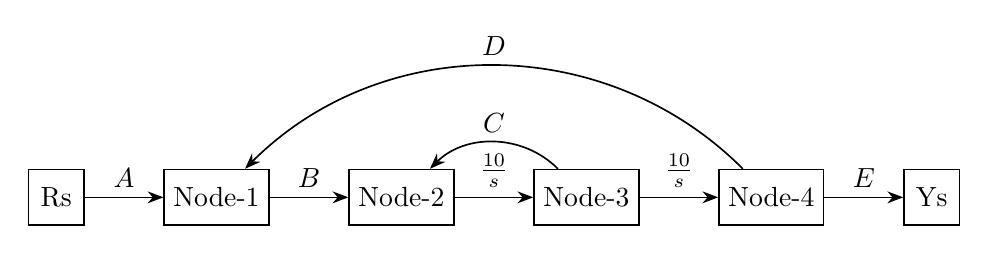
\begin{tikzpicture}[>=Stealth,auto,node distance=1cm,semithick]
  \tikzstyle{block}=[draw, fill=white, rectangle, minimum height=2em, minimum width=2em]
  
  \node [block] (input) {R\brak{s}};
  \node [block, right=of input] (filter) {Node-1};
  \node [block, right=of filter] (D) {Node-2};
  \node [block, right=of D] (E) {Node-3};
  \node [block, right=of E] (F) {Node-4};
  \node [block, right=of F] (output) {Y\brak{s}};
  
  \draw [->] (input) -- node {$A$} (filter);
  \draw [->] (filter) -- node {$B$} (D);
  \draw [->] (D) -- node {$\frac{10}{s}$} (E);
  \draw [->] (E) -- node {$\frac{10}{s}$} (F);
  \draw [->] (F) -- node {$E$} (output);
  
  % Backward loops
  \draw [->] (E) edge [bend right=45] node[above] {$C$} (D);
  \draw [->] (F) edge [bend right=45] node[above] {$D$} (filter);
\end{tikzpicture}%
}
\caption{Signal Flow Diagram}
\label{fig:your_label}
\end{figure}


Mason's Gain Formula is given by :
\begin{align}
    H\brak{s} = \sum_{i=1}^{N}\brak{\frac{P_i \Delta_i}{\Delta}} \label{eq:eq1_ee39}
\end{align}
\begin{table}[!ht] 
\centering
\setlength{\extrarowheight}{8pt}
\begin{tabular}{|l|l|}
    \hline
    \textbf{Parameter} & \textbf{Description}\\
    \hline
     N & Number of forward paths \\\hline
     L & Number of loops\\\hline
     $P_k$ & Forward path gain of $k^{th}$ path\\\hline
     $\Delta_k$ & Associated path factor \\\hline
     $\Delta$ & Determinant of the graph \\\hline
  \end{tabular}
  \vspace{4mm}
 \caption{Parameter Table - Mason's Gain Law}
 \label{tab:table1_ee_22_39}
\end{table}

\begin{table}[!ht] 
\centering
\setlength{\extrarowheight}{8pt}
\begin{tabular}{|l|l|}
    \hline
    \textbf{Parameter} & \textbf{Formula}\\
    \hline
     $\Delta$ & 1 + $\sum_{k=1}^{L}\brak{\brak{-1}^k\text{Product of gain of groups of k isolated loops}}$ \\\hline
     $\Delta_k$ & $\Delta$ part of graph that is not touching $k^{th}$ forward path \\\hline
  \end{tabular}
  \vspace{4mm}
 \caption{Formula Table - Mason's Gain Law}
 \label{tab:table2_ee_22_39}
\end{table}

This signal flow graph has only one forward path whose gain is given by :
\begin{align}
    P_1 &= \frac{10}{s} \frac{10}{s}\\
    &= \frac{100}{s^2}
\end{align}
The loop gain for loop between Node-2 and Node-3 is :
\begin{align}
    L_1 &= \frac{10}{s}\brak{-1}\\
    &= -\frac{10}{s}
\end{align}
The loop gain for loop between Node-1 and Node-4 is :
\begin{align}
    L_1 &= \frac{10}{s}\frac{10}{s}\brak{-1}\\
    &= -\frac{100}{s^2}
\end{align}
Using \tabref{tab:table2_ee_22_39}, $\Delta$ is :
\begin{align}
    \Delta &= 1 - \brak{-\frac{10}{s} - \frac{100}{s^2}}\\
    &= 1 + \frac{10}{s} + \frac{100}{s^2}
\end{align}
There are no two isolated loops available. Hence all further terms will b zero.\\
As both the loops are in contact with the only forward path,
\begin{align}
    \Delta_1 = 1
\end{align}
Using equation \eqref{eq:eq1_ee39} :
\begin{align}
    H\brak{s} &= \frac{\frac{100}{s^2}}{1 + \frac{10}{s} + \frac{100}{s^2}} \\
    &= \frac{100}{s^2 + 10s + 100}\label{eq:eq2_ee39}
\end{align}
Referring to \tabref{tab:table0_ee_22_39}, the general equation of the damping system is second order and can be written as :
\begin{align}
    m\ddot{y}(t) + c\dot{y}(t) + ky(t) = x(t)
\end{align}
Take the Laplace transform and solve for $\frac{Y\brak{s}}{X\brak{s}}$ :
\begin{align}
    \frac{Y\brak{s}}{X\brak{s}} &= \frac{\omega_n^2}{s^2 + 2\zeta\omega_n s + \omega_n^2}\\
\implies H\brak{s} &= \frac{\omega_n^2}{s^2 + 2\zeta\omega_n s + \omega_n^2} \label{eq:eq3_ee39}
\end{align}
Comparing equations \eqref{eq:eq2_ee39} and \eqref{eq:eq3_ee39} ,
\begin{align}
    \omega_n ^2 &= 100\\
    \implies \omega_n &= 10 \text{ rad/s} \label{eq:eq4_ee39}\\
    2\zeta \omega_n &= 10\\
    \implies \zeta &= 0.5
\end{align}
\begin{figure}[!ht]
\centering
\begin{center}
\includegraphics[width=\columnwidth]{2022/EE/39/figs/Figure_1.jpg}
\end{center}
\caption{Magnitude plot}
\end{figure}
\begin{figure}[!ht]
\centering
\begin{center}
\includegraphics[width=\columnwidth]{2022/EE/39/figs/Figure_2.jpg}
\end{center}
\caption{Phase plot}
\end{figure}

\newpage
\item In the block diagram shown in the figure, the transfer function $G=\frac{K}{\tau s+1}$ with $K>0$ and $\tau>0$. The maximum value of $K$ below which the system remains stable is \rule{1cm}{0.15mm}(rounded off to two decimal places) \hfill (GATE CH 2022) 
\begin{figure}[htbp] 
\includegraphics[width=\columnwidth]{2022/CH/58/figs/question.jpg} 
\end{figure}\\ 
\solution 
\input{2022/CH/58/ch_58.tex} 
\newpage

\item
A series RLC circuit is connected to 220 V, 50 Hz supply. For a fixed a value of R and C, the inductor L is varied to deliver the maximum current. This value 0.4A and the corresponding potential drop across the capacitor is 330 V. The value of the inductor L is ? (Rounded off to two decimal places).
\hfill{(GATE BM 2022)}\\
 \solution
 \iffalse
\let\negmedspace\undefined
\let\negthickspace\undefined
\documentclass[journal,12pt,onecolumn]{IEEEtran}
\usepackage{cite}
\usepackage{amsmath,amssymb,amsfonts,amsthm}
\usepackage{algorithmic}
\usepackage{graphicx}
\usepackage{textcomp}
\usepackage{xcolor}
\usepackage{txfonts}
\usepackage{listings}
\usepackage{enumitem}
\usepackage{circuitikz}
\usepackage{mathtools}
\usepackage{gensymb}
\usepackage{comment}
\usepackage[breaklinks=true]{hyperref}
\usepackage{tkz-euclide} 
\usepackage{listings}
\usepackage{gvv}    
\usepackage{enumitem}
\usepackage{amsmath}
\def\inputGnumericTable{}                                 
\usepackage[latin1]{inputenc}                                
\usepackage{color}                                            
\usepackage{array}                                            
\usepackage{longtable}                                       
\usepackage{calc}                                             
\usepackage{multirow}                                         
\usepackage{hhline}                                           
\usepackage{ifthen}                                           
\usepackage{lscape}
\usepackage{tabularx}

\newtheorem{theorem}{Theorem}[section]
\newtheorem{problem}{Problem}
\newtheorem{proposition}{Proposition}[section]
\newtheorem{lemma}{Lemma}[section]
\newtheorem{corollary}[theorem]{Corollary}
\newtheorem{example}{Example}[section]
\newtheorem{definition}[problem]{Definition}
\newcommand{\BEQA}{\begin{eqnarray}}
\newcommand{\EEQA}{\end{eqnarray}}
\newcommand{\define}{\stackrel{\triangle}{=}}
\theoremstyle{remark}
\newtheorem{rem}{Remark}
\begin{document}
\bibliographystyle{IEEEtran}
\vspace{3cm}

\title{GATE:2022 - BM 54 }
\author{EE23BTECH11025 - Anantha Krishnan $^{}$% <-this % stops a space
}
\maketitle
\bigskip



\section{question}

A series RLC circuit is connected to 220 V, 50 Hz supply. For a fixed a value of R and C, the inductor L is varied to deliver the maximum current. This value 0.4A and the corresponding potential drop across the capacitor is 330 V. The value of the inductor L is ? (Rounded off to two decimal places).
 



\textbf{Solutions :}
\fi




\begin{table}[ht!]
\centering
\begin{tabular}{ |c|c|c| } 
 \hline
Symbols & Description & Values  \\
\hline
 $V_s$ & Input voltage & 220 V and 50Hz\\
 \hline
 $\chi_L$ & Impedance across inductor & $j\omega L$\\
 \hline
 $\chi_C$ & Impedance across capacitor & $\frac{-j}{\omega C}$\\
 \hline
 $Z$& Impedance across the entire circuit & $\frac{1}{R+j\omega L +\frac{-j}{\omega C}}$\\
 \hline
\end{tabular}
\caption{Parameters, Descriptions, and Values}
\label{table:ee25-bm54-gate2022}
\end{table}






    
    \ctikzset{bipoles/thickness=1.2}
    \newcommand{\midlabelline}[3]{
   \node (midlabel) at ($ (#1)!.5!(#2) $) {#3};
   \draw[latex-] (#1) --  (midlabel);
   \draw[-latex] (midlabel) -- (#2);
}

\begin{center}
\begin{circuitikz}[scale=0.8]
    % Circuit
    \draw[line width=0.6]
        (1.5,5) to [sinusoidal voltage source, l_=$220V$${,}50Hz$, i=$I$] (1.5,1)
        (1.5,5) to [resistor, l_=$R$] ++(4,0) to [inductor, l_=$L$] ++(0,-4) to [capacitor, l_=$C$] +(-4,0) ;
    
    % Voltage Infos
    \midlabelline{1.5,5.5}{5.5,5.5}{$V(R)$}
    \midlabelline{6.5,5}{6.5,1}{$V(L)$}
    \midlabelline{1.5,0}{5.5,0}{$V(C)$}
    
    % Grid
    %\draw[help lines] (0,0) grid (7,6);
\end{circuitikz}
\end{center}
During maximum current$\quad\abs{Z}$ is minimum .
\begin{align}
I &= \frac{V_s}{Z}\\
 &= \frac{V_s}{R+\chi_{L}+\chi_{C}}\\ 
 &=\frac{V_s}{R+j\omega L+\frac{1}{j\omega C}}\label{eq:ee25-gate2-1}\\
\quad \abs{I}&={\frac{\quad \abs{V_s}}{\sqrt{R+\brak{\omega L-\frac{1}{\omega C}^2}}}}
\end{align}
Varying $L$ for maximum value of ${I}$ :
\begin{align}
\omega L = \frac{1}{\omega C} \label{eq:ee25-gate2-2}
\end{align}
Putting in $\eqref{eq:ee25-gate2-1}$:
\begin{align}
    I_{max} &= \frac{V_s}{R}
\end{align}
$I_{max}$ has same phase as $V_s$ (Assume $\angle{\phi})$.
For impedance across the capacitor :
\begin{align}
 \left.V_C\right|_{I=I_{max}}&= I_{max} \chi_C\\
-330\angle{\brak{90+\phi}} &= \brak{0.4\angle{\phi}}\chi_C\\
-330\angle{90} &= 0.4\chi_C\\
\implies \chi_C &= -825j\si{\ohm}
\end{align}
For value of Capacitor and inductor, using \eqref{eq:ee25-gate2-2} :
\begin{align}
L &= \frac{825}{100\pi}H\\
&\approx 2.63 \si{H}\\
C &= 3.858*10^{-6} \si{F}
\end{align}


    \begin{figure}[!ht]    
    \centering
\graphicspath{ {2022/BM/54/figs/} }
\includegraphics[width=\columnwidth]{graph_1}
\caption{ $I$ vs $L$ }
\label{graph:ee25-gate2-graph}
\end{figure}







 
 \newpage
 
 \item
 The open loop transfer function of a unity gain negative feedback system is given by $G\brak{s}= \frac{k}{s^2 +4s-5}$. The range of k for which the system is stable,is\hfill(GATE EE 2022)\\
\solution
\iffalse
\documentclass[journal,12pt,twocolumn]{IEEEtran}
\usepackage{amsmath,amssymb,amsfonts,amsthm}
\usepackage{txfonts}
\usepackage{tkz-euclide}
\usepackage{listings}
\usepackage{gvv}
\usepackage[latin1]{inputenc}
\usepackage{array}
\usepackage{pgf}
\usepackage{lmodern}
\usepackage{amsmath}
\begin{document}
\bibliographystyle{IEEEtran}

\title{GATE 2022[EE]-19}
\author{EE23BTECH11066 - Yakkala Amarnath Karthik}
\maketitle
\bibliographystyle{IEEEtran}

\textbf{Question:}\\ \\
The open loop transfer function of a unity gain negative feedback system is given by $G\brak{s}= \frac{k}{s^2 +4s-5}$. The range of k for which the system is stable,is\hfill(GATE EE 2022)\\ \\

\textbf{Solution:}\\ 
\fi
\begin{table}[ht]
  \begin{tabular}{|c|c|c|}
    \hline
    \textbf{Variable} & \textbf{Description} & \textbf{value}\\
    \hline
    $G\brak{s}$ & Open loop transfer function & $\frac{k}{s^2 +4s-5}$\\
   \hline
    1+G$\brak{s}$ & Characteristic equation & 0 \\
    \hline
    \end{tabular}
  \caption{A Table with input parameters}
  \label{tab:gate2022ee19}
\end{table}
\\
 from Table\ref{tab:gate2022ee19}\\
Characteristic equation:
\begin{align}
    1+G\brak{s}=0\\
    \implies 1+\frac{k}{s^2 +4s-5}=0\\
    \implies s^2+4s+\brak{k-5}=0
\end{align}
By routh table analysis, for a stable system:

\begin{center}
    \begin{tabular}{c|c c}
        $s^2$ & 1 & \(k-5\) \\
        $s^1$ & 4 & 0 \\
        $s^0$ & \(\frac{4\brak{k-5}-0}{4}\) & 0 \\
    \end{tabular}
\end{center}


\begin{align}
\frac{4\brak{k-5}-0}{4}>0\\
    k-5>0\\
    \implies k>5
\end{align}

\begin{figure}[ht]
    \centering
    \includegraphics[width=0.45\textwidth]{2022/EE/19/figs/bodeplot.png}
    \caption{Graph showing $k<5,k=5,k>5$}
\end{figure}
For an open transfer function to be stable, its magnitude in the bode plot should be positive for some positive frequency.\\
In the below graph we can observe that the above condition satisfies for k$>$5. 
%\end{document}

\newpage
 
 
\end{enumerate}

\section{2021}
\begin{enumerate}[label=\thechapter.\arabic*,ref=\thechapter.\theenumi]
\item A sinusoidal message signal having root mean square value of 4V and frequency of 1 kHz fed to a phase modulator with phase deviation constant 2 rad/volt. If the carrier signal is $c\brak{t} = 2\cos \brak{2\pi 10^6 t}$, the maximum instantaneous frequency of the phase modulated signal (rounded off to one decimal place) is \rule{1cm}{0.05mm} Hz. \hfill(GATE 2021 EC)\\
\solution\\
 \iffalse
\let\negmedspace\undefined
\let\negthickspace\undefined
\documentclass[journal,12pt,onecolumn]{IEEEtran}
\usepackage{cite}
\usepackage{amsmath,amssymb,amsfonts,amsthm}
\usepackage{algorithmic}
\usepackage{graphicx}
\usepackage{textcomp}
\usepackage{xcolor}
\usepackage{txfonts}
\usepackage{listings}
\usepackage{enumitem}
\usepackage{mathtools}
\usepackage{gensymb}
\usepackage{comment}
\usepackage[breaklinks=true]{hyperref}
\usepackage{tkz-euclide} 
\usepackage{tikz}
\usepackage{circuitikz}
%\usetikzlibrary{circuits.ee.IEC}
\usepackage{listings}
\usepackage{gvv} 
\usepackage{caption}
\def\inputGnumericTable{}                   

%\usepackage[latin1]{inputenc}                                
\usepackage{color}                                            
\usepackage{array}                                            
\usepackage{longtable}                                       
\usepackage{calc}                                             
\usepackage{multirow}                                         
\usepackage{hhline}                                           
\usepackage{ifthen}                                           
\usepackage{lscape}
\usepackage{tikz}
\usepackage{circuitikz}

\newtheorem{theorem}{Theorem}[section]
\newtheorem{problem}{Problem}
\newtheorem{proposition}{Proposition}[section]
\newtheorem{lemma}{Lemma}[section]
\newtheorem{corollary}[theorem]{Corollary}
\newtheorem{example}{Example}[section]
\newtheorem{definition}[problem]{Definition}
\newcommand{\BEQA}{\begin{eqnarray}}
\newcommand{\EEQA}{\end{eqnarray}}
\newcommand{\define}{\stackrel{\triangle}{=}}
\theoremstyle{remark}
\newtheorem{rem}{Remark}

\begin{document}

\bibliographystyle{IEEEtran}
\vspace{3cm}

\title{GATE: EE - 59.2022}
\author{EE23BTECH11013 - Avyaaz$^{*}$% <-this % stops a space 
}
\maketitle
% \newpage
% \bigskip

\renewcommand{\thefigure}{\arabic{figure}}
\renewcommand{\thetable}{\arabic{table}}

\large\textbf{\textsl{Question:}}
For the ideal AC-DC rectifier circuit shown in the figure below, the load current
magnitude is $I_{dc}$ = $15$ A and is ripple free. The thyristors are fired with a delay angle
of 45\degree
. The amplitude of the fundamental component of the source current, in
amperes, is \_\_\_\_\_\_\_\_{\em (Round off to 2
decimal places)}. \hfill(GATE 59 EE 2022)
\begin{figure}[!h]
\centering
\begin{circuitikz}[american voltages]
    \draw (0,0) node[op amp] (opamp) {};
    \draw (opamp.+) node[above]{$v_{+}$} to (-2,-0.5);
    \draw (opamp.-) node[above]{$v_{-}$} to (-2, 0.5);
    \draw (opamp.out) to (2, 0)node[right]{$v_{out}$};
    \draw (opamp.down) to (-0.1, -1) node[below]{$-v_{EE}$};
    \draw (opamp.up) to (-0.1, 1)node[above]{$+v_{DD}$};
    \draw (-2,0.5) to [R, l_=$R_1$](-3,0.5) to (-3.5, 0.5) to [V, l_=$0.1v$] (-3.5, -2) node[ground]{};
    \draw (-2, -0.5) to [R, l=$R_2$] (-2, -2) node[ground]{};
    \draw (-1.5,0.5) to (-1.5, 2) to [C, l=$C_1$] (1.5, 2) to (1.5, 0);
\end{circuitikz}

\end{figure}

\solution
\fi
\begin{table}[htbp]
\setlength{\extrarowheight}{4pt}
\setlength{\tabcolsep}{3pt}
\centering
\begin{tabular}{|c|c|c|}
\hline
\textbf{Parameter} & \textbf{Description}&\textbf{Value}\\
\hline 
$I_{dc}$& Load current & $15$A  \\
\hline
$\alpha$ &Firing angle&$45\degree$ \\
\hline
\end{tabular}

\caption{}
\label{tab:inputs.EE.59.2022}
\end{table}
% It is a Single phase symmetrical semi-converter.
% \begin{enumerate}[label={\roman*)}]
%     \item Load current magnitude $\brak{I_{dc}}$ = $15$A
%     \item Firing angle $\brak{\alpha} = 45\degree$
% \end{enumerate}
A symmetrical single phase semi converter is shown below,

\begin{figure}[!h]
\centering
    \begin{circuitikz}[scale = 0.8]
      \draw (-0.8,0.8) -- (-0.8,0.8) node[above]{$+$};
    \draw (0,2) to[sV,l=$V_s$] (0,-1);
     \draw (-0.8,0) -- (-0.8,0) node[below]{$-$};
    \draw (0,2) -- (2,2);
    \draw (2,2) -- (2,1);
    \draw (2,1) -- (3,1);
     \draw (3,1) to [thyristor] (3,3);
     \node at (2.4,2.3) {$T_1$};
    \draw (3,3) -- (5,3);
    \draw (5,1) to [thyristor] (5,3);
     \node at (4.4,2.3) {$T_2$};
    \draw (5,3) -- (7,3);
    \draw (7,3) to[resistor](7,1);
    \draw (7,1) -- (7,0);
    \draw(7,0) to [L](7,-2);
    \draw (7,-2) -- (3,-2);

    \draw (0, -1) -- (2,-1);
    \draw (2,-1) -- (2,0.4);
    \draw (2,0.4) -- (5,0.4);
    \draw (3,-2) to [Do] (3,0.4);
    \node at (3.8,-1) {$D_1$};
    \draw (3,0.4) -- (3,1);
    \draw (5,-2) to [Do] (5,0.4);
    \node at (5.8,-1) {$D_2$};
    \draw (5,0.4) -- (5,1);

     \draw[->] (6.5, 2) -- (6.5, 1) node[midway, left]{$I_{dc}$};
          \draw[->] (0.5, 2) -- (1, 2) ;
          \node at (1,1.6) {$I_s$};
          \node at (7.4,2) {$R$};
          \node at (7.4,-1.1) {$L$};

     \draw (8,2.8) -- (8,2.8) node[above]{$+$};
     \draw[->] (8,0.8) -- (8,2.8);
     \node at (8,0.5) {$V_o$};
     \draw[->] (8,0.2) -- (8,-1.8);
     \draw (8,-1.8) -- (8,-1.8) node[below]{$-$};
        \end{circuitikz}

\end{figure}

The Fourier series representation of supply current is given by:
\begin{align}
    i_s(t) = a_o +\sum_{n=1}^{\infty}C_n\sin({n\omega t} + \theta_n)\label{eq:gen_i_s}
\end{align}
 where,
 \begin{align}
 a_o &= \frac{1}{2\pi} \int_{0}^{2\pi} i_s(t)d\omega t \\
     C_n &= \sqrt{a_n^2 + b_n ^2}\label{eq:bino_coeff}\\
     \theta_n &= \tan^{-1}\left({\frac{a_n}{b_n}}\right)\label{eq: theta}
 \end{align}
\begin{align}
  \implies  a_o &= \frac{1}{2\pi}\int_{\alpha}^{\pi} I_o d\omega t - \int_{\pi + \alpha}^{2\pi} I_o d\omega t = 0\\
 \implies   a_n &= \frac{1}{\pi} \int_{\alpha}^{\pi}I_o\cos n\omega t d\omega t - \int_{\pi + \alpha}^{2\pi} I_o\cos{n\omega td\omega t}\\
 a_n &= 
 \begin{cases}
    \frac{-2I_o}{n\pi}\sin{n\alpha} & \text{for } n = 1,3,5...\\
     0 &\text{for } n = 2,4.....
    \end{cases}\\
 \implies   b_n &= \frac{1}{\pi}\int_{\alpha}^{\pi}I_o\sin n\omega t d\omega t - \int_{\pi + \alpha}^{2\pi} I_o\sin{n\omega td\omega t} \\
 b_n &= 
 \begin{cases}
     \frac{2I_o}{n\pi}\left(1 + \cos{n\alpha}\right) &\text{for } n = 1,3,5...\\
     0 &\text{for } n = 2, 4....
    \end{cases}
    \end{align}
From \eqref{eq:bino_coeff}:
\begin{align}
  \therefore  C_n &= \frac{2\sqrt{2}I_o}{n\pi}\left(\sqrt{1 + \cos{n\alpha}}\right)\\
  \implies  C_n &= \frac{4I_o}{n\pi}\cos{\frac{n\alpha}{2}}\label{eq:final_bino}
\end{align}
From \eqref{eq: theta}:
\begin{align}
    \theta_n &= \tan^{-1}\left(\frac{-\sin{n\alpha}}{1 + \cos{n\alpha}}\right)\\
    \implies \theta_n &= \frac{-n\alpha}{2}\label{eq:final_theta}
\end{align}

From \eqref{eq:gen_i_s},\eqref{eq:final_bino} and \eqref{eq:final_theta}:
\begin{align}
I_{s}(t) = \sum_{n=1,3,5...}^{\infty} \frac{4I_{o}}{n\pi}\cos{\frac{n\alpha}{2}}\sin{\left(n\omega t - \frac{n\alpha}{2}\right)}
\end{align}
% \begin{align}
% I_{s}(t) = \sum_{n=1,3,5...}^{\infty} \frac{4I_{dc}}{n\pi}\cos{\frac{n\alpha}{2}}\sin{\left(n\omega t - \frac{n\alpha}{2}\right)}
% \end{align}


% \begin{tikzpicture}[scale=1]
%     \draw[->] (0,0) -- (10,0) node[right] {$\omega t$};
%     \draw[->] (0,-2) -- (0,2) node[above] {$y$};
%     \draw[domain=0:10, smooth, variable=\x, black] plot ({\x},{sin(deg(\x))});
%     \foreach \x/\xtext in {1.57/\frac{\pi}{2},3.14/\pi,4.71/\frac{3\pi}{2},6.28/2\pi,7.85/\frac{7\pi}{2}} {
%         \draw (\x cm,0) -- (\x cm,0.1) node[below] {$\xtext$};
%     }
%     \foreach \y in {-1,1} {
%         \draw (1pt,\y cm-1.5) -- (-1pt,\y cm-1.5) node[left] {$\y$};
%     }
% \end{tikzpicture}

\begin{figure}[!h]
    \centering
    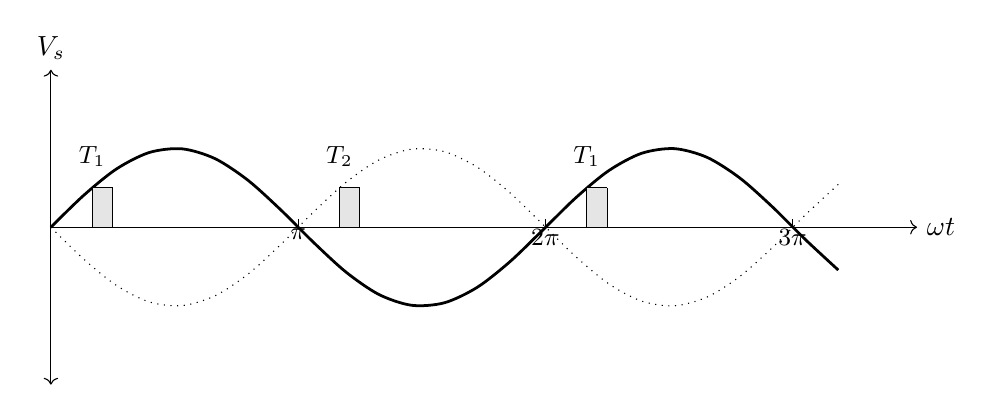
\begin{tikzpicture}[scale=1]
    \draw[->] (0,0) -- (11,0) node[right] {$\omega t$};
    \draw[<->] (0,-2) -- (0,2) node[above] {$V_s$};
    \draw[domain=0:10, smooth, variable=\x, black,line width=1pt] plot ({\x},{sin(deg(\x))});
    \draw[dotted,domain=0:10, smooth, variable=\x, black] plot ({\x},{-sin(deg(\x))});
    \foreach \x/\xtext in {3.14/\pi,6.28/2\pi,9.42/3\pi} {
        \draw (\x cm,0) -- (\x cm,0.1) node[below] {\small$\xtext$};
    }

\fill[gray!20] (0.5233,0) -- (0.5233,0.5) -- (0.785,0.5) -- (0.785,0) -- cycle;
    \fill[gray!20] (3.6633,0) -- (3.6633,0.5) -- (3.925,0.5) -- (3.925,0) -- cycle;
    \fill[gray!20] (6.8033,0) -- (6.8033,0.5) -- (7.065,0.5) -- (7.065,0) -- cycle;

    \draw (0.5233,0) -- (0.5233,0.5);
    \draw (0.5233,0.5) -- (0.785,0.5);
    \draw (0.785,0.5) -- (0.785,0);

    \draw (3.6633,0) -- (3.6633,0.5);
    \draw (3.6633,0.5) -- (3.925,0.5);
    \draw (3.925,0.5) -- (3.925,0);

    \draw (6.8033,0) -- (6.8033,0.5);
    \draw (6.8033,0.5) -- (7.065,0.5);
    \draw (7.065,0.5) -- (7.065,0);


     \node at (0.5233,0.9) {\small$T_1$};
     \node at (3.6633,0.9) {\small$T_2$};
     \node at (6.8033,0.9) {\small$T_1$};
\end{tikzpicture}
\end{figure}
\begin{figure}[!h]
    \centering
    \begin{tikzpicture}[scale=1]
    \draw[->] (0,0) -- (11,0) node[right] {$\omega t$};
    \draw[<->] (0,-2) -- (0,2) node[above] {$V_o$};
    \draw[domain=0.5233:3.14, smooth, variable=\x, black,line width=1pt] plot ({\x},{sin(deg(\x))});
    \draw[domain=3.6633:6.28, smooth, variable=\x, black,line width=1pt] plot ({\x},{-sin(deg(\x))});
    \draw[domain=6.8033:9.42, smooth, variable=\x, black,line width=1pt] plot ({\x},{sin(deg(\x))});

    \foreach \x/\xtext in {0.5233/\alpha, 3.14/\pi,4/\pi + \alpha ,6.28/2\pi,7.2/2\pi + \alpha,9.42/3\pi}{
        \draw (\x cm,0) -- (\x cm,0) node[below] {\small $\xtext$};
    }

     \draw [line width=1pt](0,0)--(0.5233,0);
    \draw [line width=1pt](0.5233,0) -- (0.5233,0.5);
    \draw[line width=1pt](3.14,0)-- (3.6633,0);
    \draw[line width=1pt] (3.6633,0) -- (3.6633,0.5);
    \draw [line width=1pt](6.28,0)--(6.8033,0);
    \draw [line width=1pt](6.8033,0) -- (6.8033,0.5);

    \node at (0.25,0.6){\small$T_2$};
    \node at (0.25,0.2){\small$D_2$};
     \node at (3.4,0.6){\small$T_1$};
    \node at (3.4,0.2){\small$D_1$};
    \node at (6.4,0.6){\small$T_2$};
    \node at (6.4,0.2){\small$D_2$};

    \node at (1.57,0.4){\small $T_1D_2$};
    \node at (4.71,0.4){\small $T_2D_1$};
    
\end{tikzpicture}
\end{figure}
\begin{figure}[!h]
    \centering
    \begin{tikzpicture}[scale=1]
    \draw[->] (0,0) -- (11,0) node[right] {$\omega t$};
    \draw[<->] (0,-2) -- (0,2) node[above] {$i_{T_1}$};
   
    \foreach \x/\xtext in {0.5233/\alpha,4/\pi + \alpha,7.2/2\pi + \alpha,10/3\pi + \alpha}{
        \draw (\x cm,0) -- (\x cm,0) node[below] {\small $\xtext$};
    }
     \draw [line width=1pt](0,0)--(0.5233,0);
    \draw [line width=1pt](0.5233,0) -- (0.5233,1);
    \draw[line width=1pt](0.5233,1)-- (3.6633,1);
    \draw[line width=1pt] (3.6633,1) -- (3.6633,0);
    \draw[line width=1pt] (3.6633,0) -- (6.8033,0);
    \draw [line width=1pt](6.8033,0)--(6.8033,1);
    \draw [line width=1pt](6.8033,1) -- (9.948,1);
     \draw [line width=1pt] (9.948,1) -- (9.948,0);

     \draw[dotted,domain=0:10, smooth, variable=\x, black] plot ({\x},{1});
     \node at (0.4,1.2) {\small $I_{DC}$};
\end{tikzpicture}
\end{figure}
\begin{figure}[!h]
    \centering
    \begin{tikzpicture}[scale=1]
    \draw[->] (0,0) -- (11,0) node[right] {$\omega t$};
    \draw[<->] (0,-2) -- (0,2) node[above] {$i_{s}$};
   

    \draw [line width=1pt](0.5233,0) -- (0.5233,1);
    \draw[line width=1pt](0.5233,1)-- (3.14,1);
    \draw[line width=1pt](3.14,1)-- (3.14,0);
    \draw[line width=1pt] (3.14,0) -- (3.6633,0);
    \draw[line width=1pt] (3.6633,0) -- (3.6633,-1);
    \draw[line width=1pt] (3.6633,-1) -- (6.28,-1);
    \draw[line width=1pt]  (6.28,-1) -- (6.28,0);
    \draw[line width=1pt] (6.28,0) -- (6.8033,0);
    \draw [line width=1pt](6.8033,0)--(6.8033,1);
    \draw [line width=1pt](6.8033,1) -- (9.42,1);
     \draw [line width=1pt] (9.42,1) -- (9.42,0);
     \draw [line width=1pt] (9.42,0) -- (9.948,0);

     \draw[dotted,domain=0:10, smooth, variable=\x, black] plot ({\x},{1});
     \node at (0.4,1.2) {\small $I_{DC}$};
    
\end{tikzpicture}
\end{figure}

From \tabref{tab:inputs.EE.59.2022}:
\begin{align}
   (I_{s_1})_{peak} &= \frac{4I_{dc}}{\pi}\cos{\left(\frac{\alpha}{2}\right)}\\
    &= \frac{4 \times 15 }{\pi}\times \cos{\frac{45 \degree}{2}}\\
    &=17.64 A 
\end{align}

%\end{document}

\pagebreak
\item Two discrete-time linear time-invarient systems with impulse responses $h_1[n]=\delta[n-1]+\delta[n+1]$ and $h_2[n]=\delta[n]+\delta[n-1]$ are connected in cascade, where $\delta[n]$ is the Kronecker delta. The impulse response of the cascaded system is   \\
\begin{enumerate}[label=(\alph*)]
    \item $\delta[n-2]+\delta[n+1]$
    \item $\delta[n-1]\delta[n]+\delta[n+1]\delta[n-1]$
    \item $\delta[n-2]+\delta[n-1]+\delta[n]+\delta[n+1]$
    \item $\delta[n]\delta[n-1]+\delta[n-2]\delta[n+1]$
\end{enumerate} \hfill(GATE 2021 EE)\\
\solution
% \iffalse
\let\negmedspace\undefined
\let\negthickspace\undefined
\documentclass[journal,12pt,twocolumn]{IEEEtran}
\usepackage{cite}
\usepackage{amsmath,amssymb,amsfonts,amsthm}
\usepackage{algorithmic}
\usepackage{graphicx}
\usepackage{textcomp}
\usepackage{xcolor}
\usepackage{pgfplots}
\usepackage{txfonts}
\usepackage{listings}
\usepackage{enumitem}
\usepackage{mathtools}
\usepackage{gensymb}
\usepackage{comment}
\usepackage[breaklinks=true]{hyperref}
\usepackage{tkz-euclide} 
\usepackage{listings}
\usepackage{gvv}                                        
\def\inputGnumericTable{}                                 
\usepackage[latin1]{inputenc}                                
\usepackage{color}                                            
\usepackage{array}                                            
\usepackage{longtable}                                       
\usepackage{calc}                                             
\usepackage{multirow}                                         
\usepackage{hhline}                                           
\usepackage{ifthen}                                           
\usepackage{lscape}

\newtheorem{theorem}{Theorem}[section]
\newtheorem{problem}{Problem}
\newtheorem{proposition}{Proposition}[section]
\newtheorem{lemma}{Lemma}[section]
\newtheorem{corollary}[theorem]{Corollary}
\newtheorem{example}{Example}[section]
\newtheorem{definition}[problem]{Definition}
\newcommand{\BEQA}{\begin{eqnarray}}
\newcommand{\EEQA}{\end{eqnarray}}
\newcommand{\define}{\stackrel{\triangle}{=}}
\theoremstyle{remark}
\newtheorem{rem}{Remark}
\begin{document}
\parindent 0px
\bibliographystyle{IEEEtran}
\title{GATE: EE - 7.2021}
\author{EE22BTECH11219 - Rada Sai Sujan$^{}$% <-this % stops a space
}
\maketitle
\newpage
\bigskip
\section*{Question}
Two discrete-time linear time-invarient systems with impulse responses $h_1[n]=\delta[n-1]+\delta[n+1]$ and $h_2[n]=\delta[n]+\delta[n-1]$ are connected in cascade, where $\delta[n]$ is the Kronecker delta. The impulse response of the cascaded system is   \\
\begin{enumerate}[label=(\alph*)]
    \item $\delta[n-2]+\delta[n+1]$
    \item $\delta[n-1]\delta[n]+\delta[n+1]\delta[n-1]$
    \item $\delta[n-2]+\delta[n-1]+\delta[n]+\delta[n+1]$
    \item $\delta[n]\delta[n-1]+\delta[n-2]\delta[n+1]$
\end{enumerate} \hfill(GATE 2021 EE)\\
\solution

\begin{figure}[ht]
    \centering
    \includegraphics[width=\columnwidth]{figs/fig2.png}
    \caption{Block Diagram}
    \label{fig:g2022ee7.2}
\end{figure}  
From the $Z$-transformation pairs,
\begin{align}
    \delta[n] &\overset{\mathcal{Z}}{ \longleftrightarrow} 1  \label{eqn:g22ee7.1}  \\
    x\brak{n-k} &\overset{\mathcal{Z}}{ \longleftrightarrow} z^{-k}X\brak{z} \label{eqn:g22ee7.2}   \\
    x_1\brak{n}\ast x_2\brak{n} &\overset{\mathcal{Z}}{ \longleftrightarrow} X_1\brak{z}X_2\brak{z} \label{eqn:g22ee7.3}
\end{align}
If $h_1\brak{n}$ and $h_2\brak{n}$ are cascade connected then the resultant impulse can be given by:
\begin{align}
    h\brak{n}&=h_1\brak{n}\ast h_2\brak{n}    \\
    \implies H\brak{z}&=H_1\brak{z}H_2\brak{z}    \\
    H\brak{z}&=\brak{z^{-1}+z}\brak{1+z^{-1}}   \\
    &=\brak{z^{-1}+z^{-2}+z+1}, \quad \abs{z}\neq 0
\end{align}
Using the $Z$-transformation pairs to find the the inverse $Z$-transform,
\begin{align}
    h\brak{n}&=\delta[n-2]+\delta[n-1]+\delta[n]+\delta[n+1]
\end{align}
\begin{figure}[ht]
    \centering
    \includegraphics[width=\columnwidth]{figs/fig3.png}
    \caption{$h_1\brak{n}$ $vs$ $n$ graph}
    \label{fig:g2022ee7.3}
\end{figure}     
\begin{figure}[ht]
    \centering
    \includegraphics[width=\columnwidth]{figs/fig4.png}
    \caption{$h_2\brak{n}$ $vs$ $n$ graph}
    \label{fig:g2022ee7.4}
\end{figure}     
\begin{figure}[ht]
    \centering
    \includegraphics[width=\columnwidth]{figs/fig1.png}
    \caption{$h\brak{n}$ $vs$ $n$ graph}
    \label{fig:g2022ee7.1}
\end{figure}        
\end{document}

\pagebreak
\item Consider a superheterodyne receiver tuned to 600 kHz. If the local oscillator feeds a 1000 kHz signal to the mixer, the image frequency (in integer) is \underline{\hspace{1cm}} kHz.
\hfill(GATE EC 2021)\\
\solution
\documentclass{article}
\usepackage{tikz}
\usetikzlibrary{positioning, arrows.meta, shapes.geometric, shapes.multipart}
\usepackage{amsmath}

\begin{document}

Consider a superheterodyne receiver tuned to 600 kHz. If the local oscillator feeds a 1000 kHz signal to the mixer, the image frequency (in integer) is \underline{\hspace{1cm}} kHz.
\hfill(GATE EC 2021)\\

\textbf{Solution:}
\begin{table}[h]
    \centering
    \begin{tabular}{|c|c|c|}
        \hline
        \textbf{Parameter} & \textbf{Symbol} & \textbf{Value} \\
        \hline
        Receiver Frequency & \(f_r\) & 600 kHz \\
        \hline
        Local Oscillator Frequency & \(f_l\) & 1000 kHz \\
        \hline
        Image Frequency & \(f_i\) & \underline{\hspace{2cm}} kHz \\
        \hline
    \end{tabular}
    \caption{Given Parameters with Symbols}
    \label{tab:receiver_parameters}
\end{table}

Let \(f_x\) be the intermediate frequency given by \(|f_l - f_r|\).
\begin{align}
    f_x &= |1000-600| = 400 \, \text{kHz}
\end{align}
\begin{figure}[htb]
 \centering
\begin{tikzpicture}
    \draw (0,0) -- (6,0);
    \draw[thick,->] (1,0) -- node[below=4mm] {$f_r$} (1,1);
    \draw[thick,->] (3,0) -- node[below=14mm] {$f_l$} (3,3);
    \draw[thick,->] (5,0) --  node[below=4mm] {$f_i$}(5,1);
    \draw[<->] (1.25,0.5) --node[above] {$f_x$}(2.75,0.5);
    \draw[<->] (3.25,0.5) --node[above] {$f_x$}(4.75,0.5);
\end{tikzpicture}
 \caption{Diagram}
    \label{fig:reflection}
\end{figure}



From the above diagram, we can observe that:
\begin{align}
    f_i &= f_r+2(f_x) = 600+2(400)=1400 \, \text{kHz}
\end{align}
Therefore the Image frequency is \textbf{1400 kHz}
\begin{figure}
    \centering
    \begin{tikzpicture}[
        block/.style={draw, rectangle, minimum height=1.5cm, text width=3cm, align=center},
        arrow/.style={->, >=Stealth},
        node distance=2cm
    ]

    % Nodes
    \node[block] (mixer) {Mixer};
    \node[block, below=of mixer] (if) {Intermediate\\Frequency\\($f_x = 400$ kHz)};
    \node[block, below=of if] (lo) {Local Oscillator\\($f_r = 1000$ kHz)};
    \node[block, below=of lo] (rf) {RF Signal\\($f_l = 600$ kHz)};
    \node[block, right=of if, xshift=2cm] (image) {Image Frequency\\($f_i = 1400$ kHz)};

    % Arrows
    \draw[arrow] (rf) -- (lo);
    \draw[arrow] (lo) -- (if);
    \draw[arrow] (mixer) -- (if);
    \draw[arrow] (if) -- (image);

    \end{tikzpicture}
    \caption{Superheterodyne Receiver Block Diagram}
    \label{fig:blockdiagram}
\end{figure}


\end{document}


\pagebreak
\item Consider a unity feedback system with closed loop transfer function
\begin{align*}
\frac{C\brak{s}}{R\brak{s}} &= \frac{s + 90}{s^2 + 10s + 90}
\end{align*}
The steady state error with respect to a unit ramp input is \rule{1cm}{0.15mm} .
\hfill(GATE 2021 BM) \\
\solution
\iffalse
\let\negmedspace\undefined
\let\negthickspace\undefined
\documentclass[journal,12pt,twocolumn]{IEEEtran}
\usepackage{cite}
\usepackage{amsmath,amssymb,amsfonts,amsthm}
\usepackage{algorithmic}
\usepackage{graphicx}
\usepackage{textcomp}
\usepackage{xcolor}
\usepackage{txfonts}
\usepackage{listings}
\usepackage{enumitem}
\usepackage{mathtools}
\usepackage{gensymb}
\usepackage{comment}
\usepackage[breaklinks=true]{hyperref}
\usepackage{tkz-euclide}
\usepackage{listings}
\usepackage{gvv}
\def\inputGnumericTable{}
\usepackage[latin1]{inputenc}
\usepackage{color}
\usepackage{array}
\usepackage{longtable}
\usepackage{calc}
\usepackage{multirow}
\usepackage{hhline}
\usepackage{ifthen}
\usepackage{lscape}

\newtheorem{theorem}{Theorem}[section]
\newtheorem{problem}{Problem}
\newtheorem{proposition}{Proposition}[section]
\newtheorem{lemma}{Lemma}[section]
\newtheorem{corollary}[theorem]{Corollary}
\newtheorem{example}{Example}[section]
\newtheorem{definition}[problem]{Definition}
\newcommand{\BEQA}{\begin{eqnarray}}
\newcommand{\EEQA}{\end{eqnarray}}
\newcommand{\define}{\stackrel{\triangle}{=}}
\theoremstyle{remark}
\newtheorem{rem}{Remark}
\begin{document}

\bibliographystyle{IEEEtran}
\vspace{3cm}

\title{GATE 2021 BM 46}
\author{EE23BTECH11007 - Aneesh Kadiyala$^{*}$% <-this % stops a space
}
\maketitle
\newpage
\bigskip

\renewcommand{\thefigure}{\theenumi}
\renewcommand{\thetable}{\theenumi}

\vspace{3cm}
\textbf{Question:} Consider a unity feedback system with closed loop transfer function
\begin{align*}
\frac{C\brak{s}}{R\brak{s}} &= \frac{s + 90}{s^2 + 10s + 90}
\end{align*}
The steady state error with respect to a unit ramp input is \rule{1cm}{0.15mm} . \brak{\text{rounded off to one decimal}}

\hfill(GATE 2021 BM)
\\
\solution
\\
\fi
\begin{figure}[h!]
\centering
\includegraphics[width=\columnwidth]{2021/BM/46/figs/block-diagram.pdf}
\caption{Block Diagram of the System}
\label{fig:2021bm46-1}
\end{figure}

\begin{align}
\frac{C\brak{s}}{R\brak{s}} &= \frac{s + 90}{s^2 + 10s + 90}
\end{align}
where $C\brak{s}$ is the output and $R\brak{s}$ is the input.
Given that input is unit ramp function:
\begin{align}
r\brak{t} &= tu\brak{t} \\
\implies R\brak{s} &= \frac{1}{s^2} \\
\implies C\brak{s} &= \frac{s + 90}{s^2\brak{s^2+10s+90}} \\
E\brak{s} &= R\brak{s} - C\brak{s} \\
&= \frac{s^2+9s}{s^2\brak{s^2+10s+90}}
\end{align}
Steady state error is:
\begin{align}
\lim_{s\to0}{sE\brak{s}} &= \frac{s + 9}{s^2 + 10s + 90} \\
&= \frac{1}{10}
\end{align}
$\therefore$ steady state error for unit ramp input is 0.1.
\begin{figure}[h!]
\centering
\includegraphics[width=\columnwidth]{2021/BM/46/figs/r_t.png}
\caption{Plot of $r\brak{t}$ vs $t$}
\label{fig:2021bm46-2}
\end{figure}
\begin{align}
C\brak{s} &= \frac{s + 90}{s^2\brak{s^2+10s+90}} \\
&= -\frac{1}{10s} + \frac{1}{s^2} + \frac{s}{10\brak{s^2 + 10s + 90}} \\
&= -\frac{1}{10s} + \frac{1}{s^2} + \frac{s + 5}{\brak{s+5}^2+65} - \frac{1}{2}\brak{\frac{1}{\brak{s+5}^2+65}}
\end{align}
\begin{align}
c\brak{t} &= u\brak{t}\brak{-\frac{1}{10} + t + \frac{e^{-5t}}{10} \cos{\brak{\sqrt{65}t}} - \frac{e^{-5t}}{2\sqrt{65}}\sin{\brak{\sqrt{65}t}}}
\end{align}
\begin{figure}[h!]
\centering
\includegraphics[width=\columnwidth]{2021/BM/46/figs/c_t.png}
\caption{Plot of $c\brak{t}$ vs $t$}
\label{fig:2021bm46-3}
\end{figure}
\begin{align}
E\brak{s} &= R\brak{s} - C\brak{s} \\
\implies e\brak{t} &= r\brak{t} - c\brak{t} \\
&= u\brak{t}\brak{\frac{1}{10} - \frac{e^{-5t}}{10} \cos{\brak{\sqrt{65}t}} + \frac{e^{-5t}}{2\sqrt{65}}\sin{\brak{\sqrt{65}t}}}
\end{align}
\begin{figure}[h!]
\centering
\includegraphics[width=\columnwidth]{2021/BM/46/figs/e_t.png}
\caption{Plot of $e\brak{t}$ vs $t$}
\label{fig:2021bm46-4}
\end{figure}
\begin{align}
\text{Feedback Gain } &= \frac{\frac{C\brak{s}}{R\brak{s}}}{1 + \frac{C\brak{s}}{R\brak{s}}} \\
&= \frac{s + 90}{s^2 + 11s + 180}
\end{align}
\item A unit step input is applied to a system with impulse response H\brak{s} = $\frac{1- \frac{s}{\omega{_z}}}{1+\frac{s}{\omega{_p}}}$ at t=0. The output of the system $y\brak{t}$ at t=$0^+$ is:
\begin{enumerate}[label=\alph*)]
 \item 1
 \item $-\frac{\omega{_z}}{\omega{_p}}$
 \item $-\frac{\omega{_p}}{\omega{_z}}$
 \item 0
\end{enumerate} \hfill(GATE 2021 BM)\\
\solution
\iffalse
\let\negmedspace\undefined
\let\negthickspace\undefined
\documentclass[journal,12pt,onecolumn]{IEEEtran}
\usepackage{cite}
\usepackage{amsmath,amssymb,amsfonts,amsthm}
\usepackage{algorithmic}
\usepackage{graphicx}
\usepackage{textcomp}
\usepackage{xcolor}
\usepackage{txfonts}
\usepackage{listings}
\usepackage{enumitem}
\usepackage{mathtools}
\usepackage{gensymb}
\usepackage{circuitikz}
\usepackage{tkz-euclide} % loads  TikZ and tkz-base
\usepackage{listings}
\usetikzlibrary{positioning,arrows,shapes}


\newtheorem{theorem}{Theorem}[section]
\newtheorem{problem}{Problem}
\newtheorem{proposition}{Proposition}[section]
\newtheorem{lemma}{Lemma}[section]
\newtheorem{corollary}[theorem]{Corollary}
\newtheorem{example}{Example}[section]
\newtheorem{definition}[problem]{Definition}
%\newtheorem{thm}{Theorem}[section] 
%\newtheorem{defn}[thm]{Definition}
%\newtheorem{algorithm}{Algorithm}[section]
%\newtheorem{cor}{Corollary}
\newcommand{\BEQA}{\begin{eqnarray}}
\newcommand{\EEQA}{\end{eqnarray}}
\newcommand{\system}[1]{\stackrel{#1}{\rightarrow}}

\newcommand{\define}{\stackrel{\triangle}{=}}
\theoremstyle{remark}
\newtheorem{rem}{Remark}
%\bibliographystyle{ieeetr}
\begin{document}
%
\providecommand{\pr}[1]{\ensuremath{\Pr\left(#1\right)}}
\providecommand{\prt}[2]{\ensuremath{p_{#1}^{\left(#2\right)} }}        % own macro for this question
\providecommand{\qfunc}[1]{\ensuremath{Q\left(#1\right)}}
\providecommand{\sbrak}[1]{\ensuremath{{}\left[#1\right]}}
\providecommand{\lsbrak}[1]{\ensuremath{{}\left[#1\right.}}
\providecommand{\rsbrak}[1]{\ensuremath{{}\left.#1\right]}}
\providecommand{\brak}[1]{\ensuremath{\left(#1\right)}}
\providecommand{\lbrak}[1]{\ensuremath{\left(#1\right.}}
\providecommand{\rbrak}[1]{\ensuremath{\left.#1\right)}}
\providecommand{\cbrak}[1]{\ensuremath{\left\{#1\right\}}}
\providecommand{\lcbrak}[1]{\ensuremath{\left\{#1\right.}}
\providecommand{\rcbrak}[1]{\ensuremath{\left.#1\right\}}}
\newcommand{\sgn}{\mathop{\mathrm{sgn}}}
\providecommand{\abs}[1]{\left\vert#1\right\vert}
\providecommand{\res}[1]{\Res\displaylimits_{#1}} 
\providecommand{\norm}[1]{\left\lVert#1\right\rVert}
%\providecommand{\norm}[1]{\lVert#1\rVert}
\providecommand{\mtx}[1]{\mathbf{#1}}
\providecommand{\mean}[1]{E\left[ #1 \right]}
\providecommand{\cond}[2]{#1\middle|#2}
\providecommand{\fourier}{\overset{\mathcal{F}}{ \rightleftharpoons}}
\newenvironment{amatrix}[1]{%
  \left(\begin{array}{@{}*{#1}{c}|c@{}}
}{%
  \end{array}\right)
}
\providecommand{\hilbert}{\overset{\mathcal{H}}{ \rightleftharpoons}}
\providecommand{\system}{\overset{\mathcal{H}}{ \longleftrightarrow}}
	%\newcommand{\solution}[2]{\textbf{Solution:}{#1}}
\newcommand{\solution}{\noindent \textbf{Solution: }}
\newcommand{\cosec}{\,\text{cosec}\,}
\providecommand{\dec}[2]{\ensuremath{\overset{#1}{\underset{#2}{\gtrless}}}}
\newcommand{\myvec}[1]{\ensuremath{\begin{pmatrix}#1\end{pmatrix}}}
\newcommand{\mydet}[1]{\ensuremath{\begin{vmatrix}#1\end{vmatrix}}}
\newcommand{\myaugvec}[2]{\ensuremath{\begin{amatrix}{#1}#2\end{amatrix}}}
\providecommand{\rank}{\text{rank}}
\providecommand{\pr}[1]{\ensuremath{\Pr\left(#1\right)}}
\providecommand{\qfunc}[1]{\ensuremath{Q\left(#1\right)}}
	\newcommand*{\permcomb}[4][0mu]{{{}^{#3}\mkern#1#2_{#4}}}
\newcommand*{\perm}[1][-3mu]{\permcomb[#1]{P}}
\newcommand*{\comb}[1][-1mu]{\permcomb[#1]{C}}
\providecommand{\qfunc}[1]{\ensuremath{Q\left(#1\right)}}
\providecommand{\gauss}[2]{\mathcal{N}\ensuremath{\left(#1,#2\right)}}
\providecommand{\diff}[2]{\ensuremath{\frac{d{#1}}{d{#2}}}}
\providecommand{\myceil}[1]{\left \lceil #1 \right \rceil }
\newcommand\figref{Fig.~\ref}
\newcommand\tabref{Table~\ref}
\newcommand{\sinc}{\,\text{sinc}\,}
\newcommand{\rect}{\,\text{rect}\,}
%%
%	%\newcommand{\solution}[2]{\textbf{Solution:}{#1}}
%\newcommand{\solution}{\noindent \textbf{Solution: }}
%\newcommand{\cosec}{\,\text{cosec}\,}
%\numberwithin{equation}{section}
%\numberwithin{equation}{subsection}
%\numberwithin{problem}{section}
%\numberwithin{definition}{section}
%\makeatletter
%\@addtoreset{figure}{problem}
%\makeatother

%\let\StandardTheFigure\thefigure
\let\vec\mathbf

\bibliographystyle{IEEEtran}





\bigskip

\renewcommand{\thefigure}{\theenumi}
\renewcommand{\thetable}{\theenumi}
%\renewcommand{\theequation}{\theenumi}


\title{GATE 2021 BM}
\author{Praful Kesavadas\\ EE23BTECH11049}
\maketitle

\textbf{Q:27}A unit step input is applied to a system with impulse response H\brak{s} = $\frac{1- \frac{s}{\omega{_z}}}{1+\frac{s}{\omega{_p}}}$ at t=0. The output of the system $y\brak{t}$ at t=$0^+$ is:
\begin{enumerate}[label=\alph*)]
 \item 1
 \item $-\frac{\omega{_z}}{\omega{_p}}$
 \item $-\frac{\omega{_p}}{\omega{_z}}$
 \item 0
\end{enumerate}
\solution\\
\fi
Given, input signal $$x\brak{t}= u\brak{t}$$
\begin{align}
 Y\brak{s} &= H\brak{s}.X\brak{s}\\
 &= \frac{1}{s}.\frac{1- \frac{s}{\omega{_z}}}{1+\frac{s}{\omega{_p}}}
\end{align}
By initial value theorem, 
\begin{align}
 y\brak{t=0^+} &= \lim_{s\to\infty} sY\brak{s}\\
 &= \lim_{s\to\infty} \frac{1- \frac{s}{\omega{_z}}}{1+\frac{s}{\omega{_p}}}\\
 &= \lim_{s\to\infty} \frac{\frac{1}{s}- \frac{1}{\omega{_z}}}{\frac{1}{s}+\frac{1}{\omega{_p}}}\\
 &= -\frac{\omega{_p}}{\omega{_z}}
\end{align}
Hence, option \brak{c} is correct
%\end{document}


\item In the block diagram shown below, an infinite tap FIR filter with transfer function $H\brak{z}=\frac{Y\brak{z}}{X\brak{z}}$ is realized. If $H\brak{z}=\frac{1}{1-0.5z^{-1}}$.\\the value of $\alpha$ is
\begin{figure}[h]
    \includegraphics[width=1\columnwidth]{2021/BM/31/figs/questionfig.png}
    \label{fig:question31bm}
\end{figure} \hfill(GATE 2021 BM)\\
\solution
 \iffalse
\let\negmedspace\undefined
\let\negthickspace\undefined
\documentclass[journal,12pt,twocolumn]{IEEEtran}
\usepackage{cite}
\usepackage{amsmath,amssymb,amsfonts,amsthm}
\usepackage{algorithmic}
\usepackage{graphicx}
\usepackage{textcomp}
\usepackage{xcolor}
\usepackage{txfonts}
\usepackage{listings}
\usepackage{enumitem}
\usepackage{mathtools}
\usepackage{gensymb}
\usepackage{comment}
\usepackage{tikz}
\usepackage[breaklinks=true,hidelinks]{hyperref}
\usepackage{tkz-euclide} 
\usepackage{listings}
\usepackage{gvv}
\def\inputGnumericTable{}
\usepackage[latin1]{inputenc}                              
\usepackage{color} 
\usepackage{array}                                            
\usepackage{longtable}                                       
\usepackage{calc}                                             
\usepackage{multirow}                                         
\usepackage{hhline}                                           
\usepackage{ifthen}                                           
\usepackage{lscape}

\newtheorem{theorem}{Theorem}[section]
\newtheorem{problem}{Problem}
\newtheorem{proposition}{Proposition}[section]
\newtheorem{lemma}{Lemma}[section]
\newtheorem{corollary}[theorem]{Corollary}
\newtheorem{example}{Example}[section]
\newtheorem{definition}[problem]{Definition}
\newcommand{\BEQA}{\begin{eqnarray}}
\newcommand{\EEQA}{\end{eqnarray}}
\newcommand{\define}{\stackrel{\triangle}{=}}
\theoremstyle{remark}
\newtheorem{rem}{Remark}
\begin{document}

\bibliographystyle{IEEEtran}
\vspace{3cm}

\title{GATE 2021 BM Q-31}
\author{EE23BTECH11207 -KAILASH.C$^{*}$% <-this % stops a space
}
\maketitle
\newpage
\bigskip

\renewcommand{\thefigure}{\theenumi}
\renewcommand{\thetable}{\theenumi}
In the block diagram shown below, an infinite tap FIR filter with transfer function $H\brak{z}=\frac{Y\brak{z}}{X\brak{z}}$ is realized. If $H\brak{z}=\frac{1}{1-0.5z^{-1}}$.\\the value of $\alpha$ is
\begin{figure}[h]
    \includegraphics[width=1\columnwidth]{2021/BM/31/figs/questionfig.png}
    \label{fig:question31bm}
\end{figure} \hfill(GATE 2021 BM)\\
\solution
\fi
\begin{table}[h]
\begin{tabular}{|l|l|l|}
\hline
\textbf{Parameter} & \textbf{Definition}\\ \hline
$H\brak{z} & $\frac{1}{1-0.5z^{-1}}$ \\ \hline
\end{tabular}
\caption{Parameter Table}
\label{tab:gate.bm.31.2021}
\end{table}
\\
From diagram we have:
\begin{align}
    Y\brak{z}&=X\brak{z}\brak{\sum_{n=0}^{\infty}\brak{z^{-1}\alpha^{2}}^n}\label{eq:311_bm}
\end{align}
Dividing by $X\brak{z}$ in both sides:
\begin{align}
    \frac{Y\brak{z}}{X\brak{z}}&=\sum_{n=0}^{\infty}\brak{z^{-1}\alpha^{2}}^n\label{eq:312_bm}\\
    \implies H\brak{z}&=\sum_{n=0}^{\infty}\brak{z^{-1}\alpha^{2}}^n\label{eq:313_bm}\\
    \frac{1}{1-0.5z^{-1}}&=\sum_{n=0}^{\infty}\brak{z^{-1}\alpha^{2}}^n\label{eq:314_bm}\\
\frac{1}{1-0.5z^{-1}}&=\frac{1}{1-z^{-1}\alpha^{2}}\label{eq:315_bm}\\
\implies \alpha&=\frac{1}{\sqrt{2}}\label{eq:316_bm}
\end{align}

\pagebreak
\item A unity feedback system that uses proportional-integral (PI) control is shown in the figure.
 \begin{figure}[!ht]    
    \centering
\graphicspath{ {2021/EC/48/figs} }
\includegraphics[width=\columnwidth]{figure_1}
\label{figure:ee25-gate4-graph}
\end{figure}
The stability of the overall system is controlled by tuning the PI control parameters $K_p$ and $K_i$. The maximum value of $K_i$ that can be chosen so as to keep the overall system stable or, in the worst case, marginally stable (\textit{rounded off to three decimal places}) is?
\hfill{(GATE EC 2021)}\\
\solution
\iffalse
\let\negmedspace\undefined
\let\negthickspace\undefined
\documentclass[journal,12pt,onecolumn]{IEEEtran}
\usepackage{cite}
\usepackage{amsmath,amssymb,amsfonts,amsthm}
\usepackage{algorithmic}
\usepackage{graphicx}
\usepackage{textcomp}
\usepackage{xcolor}
\usepackage{txfonts}
\usepackage{listings}
\usepackage{enumitem}
\usepackage{circuitikz}
\usepackage{mathtools}
\usepackage{gensymb}
\usepackage{comment}
\usepackage[breaklinks=true]{hyperref}
\usepackage{tkz-euclide} 
\usepackage{listings}
\usepackage{gvv}    
\usepackage{enumitem}
\usepackage{amsmath}
\def\inputGnumericTable{}                                 
\usepackage[latin1]{inputenc}                                
\usepackage{color}                                            
\usepackage{array}                                            
\usepackage{longtable}                                       
\usepackage{calc}                                             
\usepackage{multirow}                                         
\usepackage{hhline}                                           
\usepackage{ifthen}                                           
\usepackage{lscape}
\usepackage{tabularx}
\usepackage[italicdiff]{physics}
\usepackage{mathrsfs}
\usetikzlibrary{arrows,positioning}


\newtheorem{theorem}{Theorem}[section]
\newtheorem{problem}{Problem}
\newtheorem{proposition}{Proposition}[section]
\newtheorem{lemma}{Lemma}[section]
\newtheorem{corollary}[theorem]{Corollary}
\newtheorem{example}{Example}[section]
\newtheorem{definition}[problem]{Definition}
\newcommand{\BEQA}{\begin{eqnarray}}
\newcommand{\EEQA}{\end{eqnarray}}
\newcommand{\define}{\stackrel{\triangle}{=}}
\theoremstyle{remark}
\newtheorem{rem}{Remark}
\begin{document}
\bibliographystyle{IEEEtran}
\vspace{3cm}

\title{GATE:2021 - EC 48 }
\author{EE23BTECH11025 - Anantha Krishnan $^{}$% <-this % stops a space
}
\maketitle
\bigskip



\section{question}
A unity feedback system that uses proportional-integral (PI) control is shown in the figure.
 \begin{figure}[!ht]    
    \centering
\graphicspath{ {2021/EC/48/figs} }
\includegraphics[width=\columnwidth]{figure_1}
\label{figure:ee25-gate4-graph}
\end{figure}
The stability of the overall system is controlled by tuning the PI control parameters $K_p$ and $K_i$. The maximum value of $K_i$ that can be chosen so as to keep the overall system stable or, in the worst case, marginally stable (\textit{rounded off to three decimal places}) is?
\hfill{(GATE EC 2021)}\\
 



\textbf{Solutions :}
\fi
    
\begin{table}[ht!]
\centering
\begin{tabular}{ |c|c|c| } 
 \hline
Symbols & Description & Values  \\
\hline
$P(s)$ & Plant transfer function & $\frac{2}{s^3+4s^2+5s+2}$ \\
 \hline
 $C(s)$ & PI controller transfer function &$K_p+\frac{K_i}{s}$\\
 \hline
$G(s)$ & Closed loop transfer function &$\frac{P(s)C(s)}{1+P(s)C(s)}$\\
 \hline
$Z$ & Number of zeroes with positive real part in $1+P(s)C(s)$ &?\\
 \hline
 $N$ & Total number of anticlockwise encirclements about $-1+0j$ in Nyquist plot & ?\\
\hline
$P$ & Number of poles with positive real part in $P(s)C(s)$ &?\\
\hline
\end{tabular}
\caption{Parameters, Descriptions, and Values}
\label{table:ee25-ec48-gate2021}
\end{table}




    From table \ref{table:ee25-ec48-gate2021}, the characteristic equation is given as:
    \begin{align}
        1+\brak{K_p+\frac{K_i}{s}}\brak{\frac{2}{s^3+4s^2+5s+2}} &= 0\\
        s^4+4s^3+5s^2+(2+2K_p)s+2K_i &=0 \label{eq:gate 2021 eq:4}
    \end{align}
    For the system to be stable, there must be no sign changes in the first column of the routh array for the above equation. From $\eqref{eq:gate 2021 eq:4}$
    \begin{align}
    \begin{array}{c|cccc}
        s^4 & 1 & 5 & 2K_i \\
        s^3 & 4 & (2 + 2K_p) & 0 \\
        s^2 & \frac{18-2K_p}{4} & 2K_i & 0 \\
        s^1 &  \frac{\brak{\frac{18-2K_p}{4}}\brak{2 + 2K_p}-8K_i}{\frac{18-2K_p}{4}} & 0 & 0\\
        s^0 & 2K_i &0 &0 \\
        \end{array}\\
        \end{align}
        \begin{align}
            \frac{18-2K_p}{4} &> 0\\
            \implies K_p &< 9 \label{eq:gate 2021 eq:1}\\
            \frac{\brak{\frac{18-2K_p}{4}}\brak{2 + 2K_p}-8K_i}{\frac{18-2K_p}{4}} &> 0\label{eq:gate 2021 eq:2}\\
        K_i &>0 \label{eq:gate 2021 eq:3}
    \end{align}
    For marginal stability, assuming 3 cases while maximising $K_i$ and checking if the above inequalities hold.
    \begin{enumerate}
        \item $K_p=9$\\
         \begin{align}
       \brak{\lim_{K_p\to9^-} \frac{\brak{\frac{18-2K_p}{4}}\brak{2 + 2K_p}-8K_i}{\frac{18-2K_p}{4}} > 0} &\cap \brak {K_i > 0}\\
       \brak{\lim_{K_p\to9^-} -8K_i > 0} &\cap \brak{{K_i > 0}}\\
  \implies K_p=9 , \forall K_i &\epsilon (\phi)
    \end{align}
    \item  $K_i=0$\\
    \begin{align}
        \brak{\brak{\frac{18-2K_p}{4}}\brak{2 + 2K_p} > 0}  \cap \brak{K_p < 9}\\
        \implies K_i=0 , \forall K_p \epsilon (-1 , 9)
    \end{align}
    \item $\frac{\brak{\frac{18-2K_p}{4}}\brak{2 + 2K_p}-8K_i}{\frac{18-2K_p}{4}} = 0$\\
        \begin{align}
            \brak{\frac{18-2K_p}{4}}\brak{2 + 2K_p} = 8K_i\\
             -K_p^2 +8K_p + 9 = 8K_i
        \end{align}
        Vertex ($K_p=4$) satisfies $\eqref{eq:gate 2021 eq:1}$:
        \begin{align}
            K_i &= 3.125 \forall (K_p = 4 ,K_i>0)
        \end{align}
          Based on the three cases for marginal stability, the maximum value of $K_i$ is $3.125$, for $K_p = 4$.\\
          \end{enumerate}

    \begin{enumerate}
        \item Verification by plotting roots of characteristic equation:\\
        If real part of atleast 1 root is equal to zero and for the rest are less than or equal to zero, then the system is marginally stable.
\begin{figure}    
    \centering
\graphicspath{ {2021/EC/48/figs} }
\includegraphics[width=\columnwidth]{graph_1}
\label{figure:ee25-gate4-graph1}
\caption{Location of roots for $k_i=0$,$k_p=-1$}
\end{figure}

\begin{figure}    
    \centering
\graphicspath{ {2021/EC/48/figs} }
\includegraphics[width=\columnwidth]{graph_2}
\caption{Location of roots for $k_i=0$,$k_p=9$}
\label{figure:ee25-gate4-graph2}
\end{figure}

\begin{figure}    
    \centering
\graphicspath{ {2021/EC/48/figs} }
\includegraphics[width=\columnwidth]{graph_3}
\caption{Location of roots for $k_i=3.125$,$k_p=4$}
\label{figure:ee25-gate4-graph3}
\end{figure}

 \item Verification by Nyquist diagrams:\\
 From $\ref{table:ee25-ec48-gate2021}$, if $P=0$ and $-1+0j$ is neither bounded nor unbounded by the contour, then the system is marginally stable.
 For P:
 \begin{align}
     s^4+4s^3+5s^2+2s &= 0\\
     (s+1)^2(s+2) &= 0\\
     \implies P &= 0\\ 
     \implies Z &= N
 \end{align}
 
 
 \begin{figure}[!ht]    
    \centering
\graphicspath{ {2021/EC/48/figs} }
\includegraphics[width=\columnwidth]{plot_1}
\label{figure:ee25-gate4-nyquist1}
\caption{ Nyquist plot for $k_i=0$,$k_p=-1$}
\end{figure}

\begin{figure}[!ht]    
    \centering
\graphicspath{ {2021/EC/48/figs} }
\includegraphics[width=\columnwidth]{plot_2}
\label{figure:ee25-gate4-nyquist2}
\caption{Nyquist plot for $k_i=0$,$k_p=9$}
\end{figure}

\begin{figure}[!ht]    
    \centering
\graphicspath{ {2021/EC/48/figs} }
\includegraphics[width=\columnwidth]{plot_3}
\label{figure:ee25-gate4-nyquist3}
\caption{Nyquist plot for for $k_i=3.125$,$k_p=4$}
\end{figure}
     \end{enumerate}

  
   
    



\pagebreak
\item In the given figure, plant $G_p(s)=\frac{2.2}{(1+0.1s)(1+0.4s)(1+1.2s)}$ and compensator $G_c(s)=K\brak{\frac{1+T_1s}{1+T_2s}}$ . The external disturbance input is D(s). It is desired that when the disturbance is a unit step, the steady-state error should not exceed 0.1 unit. The minimum value of K is 
\hfill{(GATE EE 2021)}\\
\begin{figure}[h!]
    \centering
    \includegraphics[width=\columnwidth]{2021/EE/47/figs/fig.png}
    \caption{}
    \label{fig:sr40}
\end{figure}
\\
\solution
\iffalse
\documentclass[journal,12pt,twocolumn]{IEEEtran}
\usepackage{cite}
\usepackage{amsmath,amssymb,amsfonts,amsthm}
\usepackage{algorithmic}
\usepackage{graphicx}
\usepackage{textcomp}
\usepackage{xcolor}
\usepackage{txfonts}
\usepackage{listings}
\usepackage{enumitem}
\usepackage{mathtools}
\usepackage{float}
\usepackage{gensymb}
\usepackage{comment}
\usepackage[breaklinks=true]{hyperref}
\usepackage{tkz-euclide} 
\usepackage{listings}
\usepackage{gvv}                                        
\def\inputGnumericTable{}                                 
\usepackage[latin1]{inputenc}                                
\usepackage{color}                                            
\usepackage{array}                                            
\usepackage{longtable}                                       
\usepackage{calc}                                             
\usepackage{multirow}                                         
\usepackage{hhline}                                           
\usepackage{ifthen}                                           
\usepackage{lscape}
\usepackage{amsmath}
\newtheorem{theorem}{Theorem}[section]
\newtheorem{problem}{Problem}
\newtheorem{proposition}{Proposition}[section]
\newtheorem{lemma}{Lemma}[section]
\newtheorem{corollary}[theorem]{Corollary}
\newtheorem{example}{Example}[section]
\newtheorem{definition}[problem]{Definition}
\newcommand{\BEQA}{\begin{eqnarray}}
\newcommand{\EEQA}{\end{eqnarray}}
\newcommand{\define}{\stackrel{\triangle}{=}}
\theoremstyle{remark}
\newtheorem{rem}{Remark}

\usepackage{circuitikz} 

\begin{document}
{\small

\bibliographystyle{IEEEtran}
\vspace{3cm}

\title{GATE 2021 EE 47}
\author{EE23BTECH11045 - Palavelli Srija$^{*}$}

\maketitle

\bigskip

\renewcommand{\thefigure}{\theenumi}
\renewcommand{\thetable}{\theenumi}

\vspace{3cm}
\textbf{Question:} 
In the given figure, plant $G_p(s)=\frac{2.2}{(1+0.1s)(1+0.4s)(1+1.2s)}$ and compensator $G_c(s)=K\brak{\frac{1+T_1s}{1+T_2s}}$ . The external disturbance input is D(s). It is desired that when the disturbance is a unit step, the steady-state error should not exceed 0.1 unit. The minimum value of K is
\begin{figure}[h!]
    \centering
    \includegraphics[width=\columnwidth]{2021/EE/47/figs/fig.png}
    \caption{}
    \label{fig:sr40}
\end{figure}
\\
\textbf{Solution:}\\
\fi
\begin{table}[h!]
    \centering
     \begin{tabular}{|c|c|}
        \hline
        \textbf{Symbol}  & \textbf{Value} \\
        \hline
        $G_p(s)$ & $\frac{2.2}{(1+0.1s)(1+0.4s)(1+1.2s)}$\\
         \hline
        $G_c(s)$& $K\brak{\frac{1+T_1s}{1+T_2s}}$  \\
         \hline
        $|e_{ss}|$& $\leq 0.1$\\
         \hline
        $K_{min}$& ??\\
        \hline
    \end{tabular}

    \caption{Input Parameters}
    \label{tab:table_omega}
\end{table}
 
\begin{align}
\text{From \figref{fig:sr40}}\notag\\
E(s) &= R(s)-C(s) \\
\text{Assume R(s)=0}\notag\\
E(s) &= -C(s) \\
C(s) &= \brak{E(s)G_c(s)+D(s)}G_p(s) \\
-E(s) &= \brak{E(s)G_c(s)+D(s)}G_p(s) \\
E(s) &= \frac{-D(s)G_p(s)}{1+G_c(s)G_p(s)} 
\end{align}
Using final value theorem 
\begin{align}
e_{ss} &= \lim_{{t \to \infty}} e(t) = \lim_{{s \to 0}} sE(s)\\
\text{Where}\quad\mathcal{L}\{e(t)\} &= E(s) \notag\\
e_{ss} &= \lim_{{s \to 0}} sE(s) \\
&= \lim_{{s \to 0}} \left(\frac{-sD(s)G_p(s)}{1+G_c(s)G_p(s)} \right) \\
\end{align}
\begin{align}
 D(s)&=\mathcal{L}\{u(t)\}  \notag\\
&=\frac{1}{s}\\
e_{ss} &=\lim_{{s \to 0}} \left(\frac{-s\frac{1}{s}G_p(s)}{1+G_c(s)G_p(s)} \right) \\
&= \lim_{{s \to 0}} \frac{\frac{-2.2}{(1+0.1s)(1+0.4s)(1+1.2s)}}{1+K\left(\frac{1+T_1s}{1+T_2s}\right)\frac{2.2}{(1+0.1s)(1+0.4s)(1+1.2s)}} \\
&= \lim_{{s \to 0}} \frac{-2.2(1+T_2s)}{(1+0.1s)(1+0.4s)(1+1.2s)(1+T_2s)+2.2K(1+T_1s)} \\
|e_{ss}| &= \frac{2.2}{1+2.2K} \\
\text{given}\notag\\ |e_{ss}|&\leq 0.1\\
\frac{2.2}{1+2.2K} &\leq 0.1 \\
K &\geq 9.54 \\
K_{\text{min}} &= 9.54
\end{align}
    %\end{document}

\pagebreak
\item For the closed loop system shown , the transfer function $\frac{E(s)}{R(s)}$ is \\
\begin{figure}[ht]
	\centering
	\includegraphics[width=1\linewidth]{2021/EE/11/figs/questiondia.png}
\end{figure}
\begin{enumerate}[label = (\alph*)]
	\item $\frac{G}{1+GH}$
	\item $\frac{GH}{1+GH}$
	\item $\frac{1}{1+GH}$
	\item $\frac{1}{1+G}$
\end{enumerate} \hfill{(GATE EE 2021)}\\
%\iffalse
\let\negmedspace\undefined
\let\negthickspace\undefined
\documentclass[journal,12pt,twocolumn]{IEEEtran}
\usepackage{cite}
\usepackage{amsmath,amssymb,amsfonts}
\usepackage{graphicx}
\usepackage{textcomp}
\usepackage{xcolor}
\usepackage{txfonts}
\usepackage{listings}
\usepackage{enumitem}
\usepackage{mathtools}
\usepackage{gensymb}
\usepackage{comment}
\usepackage[breaklinks=true]{hyperref}
\usepackage{tkz-euclide} 
\usepackage{listings}
\usepackage{gvv}                                        
\def\inputGnumericTable{}                                 
\usepackage[latin1]{inputenc}                                
\usepackage{color}                                            
\usepackage{array}                                            
\usepackage{longtable}                                       
\usepackage{calc}                                             
\usepackage{multirow}                                         
\usepackage{hhline}                                           
\usepackage{ifthen}                                           
\usepackage{lscape}
\usepackage[export]{adjustbox}
\usepackage{pgfplots}
\newtheorem{theorem}{Theorem}[section]
\newtheorem{problem}{Problem}
\newtheorem{proposition}{Proposition}[section]
\newtheorem{lemma}{Lemma}[section]
\newtheorem{corollary}[theorem]{Corollary}
\newtheorem{example}{Example}[section]
\newtheorem{definition}[problem]{Definition}
\newcommand{\BEQA}{\begin{eqnarray}}
	\newcommand{\EEQA}{\end{eqnarray}}
\newcommand{\define}{\stackrel{\triangle}{=}}
\newtheorem{rem}{Remark}

\begin{document}
	\parindent 0px
	\bibliographystyle{IEEEtran}
	
	\vspace{3cm}
	
	\title{GATE:EE/63}
	\author{EE23BTECH11208 - Manohar K$^{*}$
	}
	\maketitle
	\newpage
	\bigskip
	
	% \renewcommand{\thefigure}{\theenumi}
	% \renewcommand{\thetable}{\theenumi}
	
	
	
\textbf{Question:} For the closed loop system shown , the transfer function $\frac{E(s)}{R(s)}$ is \\
\begin{figure}[ht]
	\centering
	\includegraphics[width=1\linewidth]{figs/questiondia.png}
\end{figure}
\begin{enumerate}[label = (\alph*)]
	\item $\frac{G}{1+GH}$
	\item $\frac{GH}{1+GH}$
	\item $\frac{1}{1+GH}$
	\item $\frac{1}{1+G}$
\end{enumerate} \hfill{(GATE EE 2021)}\\



 \noindent \textbf{Solution:}
	Given,\\
	
	\begin{table}[h]
		\centering
		
\begin{table}[h]
  \centering
  \begin{tabular}{|c|c|c|}
    \hline
Parameter & Description & Value \\ \hline
$X(z)$ & Given Sum & $\sum_{n=0}^{\infty} 3^{n+1}z^{2n}, \quad z \in \mathbb{C} $\\
\hline
$x(n)$ & Inverse Z transform of X(z) & ?\\
\hline
  \end{tabular}
  \vspace{2mm}
  \caption{GATE MA-28(2022)}
\end{table}




		\caption{Parameters}
		\label{tab:GATE.EE.2021.11}
	\end{table}
	
	\begin{align}
		C(s)&=G \times E(s)\\
		\text{Feedback signal} &= H \times C(s)
	\end{align}
	    
	
	\begin{align}
	      E(s) &= R(s) - H \times C(s)
	\end{align}
	from eq (1),     
	\begin{align}
		E(s) &= R(s) - H \times G \times E(s)
	\end{align}
	\begin{align}
		E(s) +  H \times G \times E(s) &= R(s)
		\end{align}
		\begin{align}
					\therefore \frac{E(s)}{R(s)} &= \frac{1}{1 + GH}
	\end{align} 
	
	
	
	
\end{document}

\pagebreak

Consider two 16-point sequences x\sbrak{n} and h\sbrak{n}. Let the linear convolution of x\sbrak{n} and h\sbrak{n} be denoted by y\sbrak{n}, while z\sbrak{n} denotes the 16-point inverse discrete Fourier transform \brak{IDFT} of the product of the 16-point DFTs of x\brak{n} and h\sbrak{n}. The values of k for which z\sbrak{k} = y\sbrak{k} are 
\begin{enumerate}
    \item $k = 0, 1, 2, 3, ... , 15$
    \item $k = 0$
    \item $k = 15$
    \item $k = 0$ and $k = 15$
\end{enumerate}
\hfill(GATE EC 2021)\\
\solution
\iffalse
\let\negmedspace\undefined
\let\negthickspace\undefined
\documentclass[journal,12pt,twocolumn]{IEEEtran}
\usepackage{cite}
\usepackage{amsmath,amssymb,amsfonts,amsthm}
\usepackage{algorithmic}
\usepackage{graphicx}
\usepackage{textcomp}
\usepackage{xcolor}
\usepackage{txfonts}
\usepackage{listings}
\usepackage{enumitem}
\usepackage{mathtools}
\usepackage{gensymb}
\usepackage{comment}
\usepackage[breaklinks=true]{hyperref}
\usepackage{tkz-euclide} 
\usepackage{listings}
\usepackage{gvv}                                        
\def\inputGnumericTable{}                                 
\usepackage[latin1]{inputenc}                                
\usepackage{color}                                            
\usepackage{array}                                            
\usepackage{longtable}                                       
\usepackage{calc}                                             
\usepackage{multirow}                                         
\usepackage{hhline}                                           
\usepackage{ifthen}                                           
\usepackage{lscape}
\usepackage{placeins}
\usepackage{xparse}


\newtheorem{theorem}{Theorem}[section]
\newtheorem{problem}{Problem}
\newtheorem{proposition}{Proposition}[section]
\newtheorem{lemma}{Lemma}[section]
\newtheorem{corollary}[theorem]{Corollary}
\newtheorem{example}{Example}[section]
\newtheorem{definition}[problem]{Definition}
\newcommand{\BEQA}{\begin{eqnarray}}
\newcommand{\EEQA}{\end{eqnarray}}
\newcommand{\define}{\stackrel{\triangle}{=}}
\theoremstyle{remark}
\newtheorem{rem}{Remark}

\graphicspath{ {./figs/} } 

\begin{document}

\bibliographystyle{IEEEtran}
\vspace{3cm}

\Large\title{GATE 2021 EC 5}
\large\author{EE23BTECH11032 - Kaustubh Parag Khachane $^{*}$% <-this % stops a space
}
\maketitle
\newpage
\bigskip

\renewcommand{\thefigure}{\theenumi}
\renewcommand{\thetable}{\theenumi}
\large\textbf{Question GATE 21 EC 5} :\\
Consider two 16-point sequences x\sbrak{n} and h\sbrak{n}. Let the linear convolution of x\sbrak{n} and h\sbrak{n} be denoted by y\sbrak{n}, while z\sbrak{n} denotes the 16-point inverse discrete Fourier transform \brak{IDFT} of the product of the 16-point DFTs of x\brak{n} and h\sbrak{n}. The values of k for which z\sbrak{k} = y\sbrak{k} are 
\begin{enumerate}
    \item $k = 0, 1, 2, 3, ... , 15$
    \item $k = 0$
    \item $k = 15$
    \item $k = 0$ and $k = 15$
\end{enumerate}
\hfill(GATE EC 2021)\\
\solution\\
\fi
\begin{table}[!ht] 
\centering
\setlength{\extrarowheight}{8pt}
\begin{tabular}{|l|l|}
    \hline
    \textbf{Parameter} & \textbf{Description}  \\\hline
     x\sbrak{n} & Given 16 point sequence \\\hline
     h\sbrak{n} &  Given 16 point sequence \\\hline
     y\sbrak{n} & Linear convolution of x\sbrak{n} and h\sbrak{n} \\\hline
     z\sbrak{n} & IDFT of products of DFTs of h\sbrak{n} and x\sbrak{n} \\\hline
     N & number of terms \brak{16} \\\hline
    \end{tabular}
  \vspace{4mm}
 \caption{Parameter Table}
 \label{tab:table0_ec5}
\end{table}

We can write z\sbrak{n} as ,
\begin{align}
    z\sbrak{n} = IDFT\sbrak{X\sbrak{f}H\sbrak{f}}
\end{align}
We know that product in frequency domain is convolution in time domain. However, z\sbrak{n} is not linear convolution of x\sbrak{n} and h\sbrak{n} in the time domain due to periodicity of DFT. Point-wise multiplication in the frequency domain (product of DFTs) doesn't translate directly to convolution in the time domain due to periodicity and potential aliasing.\\
z\sbrak{n} is the circular convolution of x\sbrak{n} and h\sbrak{n}. Using the formula for circular convolution,
\begin{align}
    z\sbrak{n} = \sum_{m = -\infty}^{\infty}\brak{h\sbrak{m} \sum_{p = -\infty}^{\infty}x\sbrak{n - m -pN}} \label{eq:eq1_g21ec5}
\end{align}
y\sbrak{n} is a linear convolution of x\sbrak{n} and h\sbrak{n}.
\begin{align}
    y\sbrak{n} = \sum_{m = -\infty}^{\infty} x\brak{m} h\sbrak{n-m}
\end{align}
Each term of y\sbrak{n} will be sum of products of terms of x\sbrak{n} and h\sbrak{n}. The number of terms in each summation will go from 1 for $n=1$ to 16 for $n=15$. \\
z\sbrak{n} is expressed as sum of 15 terms for all permissible values of n using $p=0$ or $p=1$ in \eqref{eq:eq1_g21ec5}.
\\ Thus,$z\sbrak{k} = y\sbrak{k}$ can be possible for only $k=15$.
\\ For $k = 15$,
\begin{align}
    y\sbrak{15} &= x\sbrak{0}h\sbrak{15} +  x\sbrak{1}h\sbrak{14} + ...  x\sbrak{15}h\sbrak{0} 
\end{align}
Using p = 0  in \eqref{eq:eq1_g21ec5},
\begin{align}
    z\sbrak{15} &= h\sbrak{0} x\sbrak{15} + h\sbrak{1} x\sbrak{14} + ... h\sbrak{15} x\sbrak{0}\\
    &=  x\sbrak{0}h\sbrak{15} +  x\sbrak{1}h\sbrak{14} + ...  x\sbrak{15}h\sbrak{0} 
\end{align}
Thus , z\sbrak{15} = y\sbrak{15}.\\
Graphically, let 
\begin{align}
    x &= \sbrak{1,2,3,4,....,16}\\
    h &= \sbrak{1,1,1,1, ... 1}
\end{align}
Then the plot for z and y is as shown bellow.
\begin{figure}[!ht]
\centering
\begin{center}
\includegraphics[width=\columnwidth]{2021/EC/5/figs/Figure_1.png}
\end{center}
\caption{Plot of y\sbrak{n} and z\sbrak{n}}
\end{figure}

\pagebreak
\item The input signal shown below \\
\input{2021/IN/44/figs/xn}\\
is passed through the filter with following taps\\
\input{2021/IN/44/figs/n}\\
The number of non-zero output samples is \underline{\hspace{1cm}}.\\
\hfill(GATE IN 2021)
\solution
\iffalse
\let\negmedspace\undefined
\let\negthickspace\undefined
\documentclass[journal,12pt,twocolumn]{IEEEtran}
\usepackage{cite}
\usepackage{amsmath,amssymb,amsfonts,amsthm}
\usepackage{algorithmic}
\usepackage{graphicx}
\usepackage{textcomp}
\usepackage{xcolor}
\usepackage{txfonts}
\usepackage{listings}
\usepackage{enumitem}
\usepackage{mathtools}
\usepackage{gensymb}
\usepackage{comment}
\usepackage[breaklinks=true]{hyperref}
\usepackage{tkz-euclide} 
\usepackage{listings}
\usepackage{gvv}
\def\inputGnumericTable{}                                 
\usepackage[latin1]{inputenc}                                
\usepackage{color}                                            
\usepackage{array}                                            
\usepackage{longtable}                                       
\usepackage{calc}                                             
\usepackage{multirow}                                         
\usepackage{hhline}                                           
\usepackage{ifthen}                                           
\usepackage{lscape}

\newtheorem{theorem}{Theorem}[section]
\newtheorem{problem}{Problem}
\newtheorem{proposition}{Proposition}[section]
\newtheorem{lemma}{Lemma}[section]
\newtheorem{corollary}[theorem]{Corollary}
\newtheorem{example}{Example}[section]
\newtheorem{definition}[problem]{Definition}
\newcommand{\BEQA}{\begin{eqnarray}}
\newcommand{\EEQA}{\end{eqnarray}}
\newcommand{\define}{\stackrel{\triangle}{=}}
\theoremstyle{remark}
\newtheorem{rem}{Remark}

\begin{document}

\bibliographystyle{IEEEtran}
\vspace{3cm}

\title{GATE IN21 44}
\author{EE23BTECH11043 - BHUVANESH SUNIL NEHETE$^{*}$% <-this % stops a space
}
\maketitle
\newpage
\bigskip

\renewcommand{\thefigure}{\theenumi}
\renewcommand{\thetable}{\theenumi}

\bibliographystyle{IEEEtran}

\textbf{Question:}
The input signal shown below \\
\input{2021/IN/44/figs/xn}\\
is passed through the filter with following taps\\
\input{2021/IN/44/figs/n}\\
The number of non-zero output samples is \underline{\hspace{1cm}}.\\

\solution
\fi
\begin{align}
    h\sbrak{n}=-\delta\sbrak{n}+2\delta\sbrak{n+1}-\delta\sbrak{n+2}
\end{align}
\begin{align}
    y\sbrak{n}&=x\sbrak{n}*h\sbrak{n}\\
    &=x\sbrak{n}*\brak{-\delta\sbrak{n}+2\delta\sbrak{n+1}-\delta\sbrak{n+2}}\\
    y\sbrak{n}&=-x\sbrak{n}+2x\sbrak{n+1}-x\sbrak{n+2}
\end{align}

\input{2021/IN/44/figs/yn}
The number of non-zero output samples is $10$.

\begin{figure}
    \centering
    \includegraphics[width=1\linewidth]{2021/IN/44/figs/fig.png}
\end{figure}

\pagebreak
\end{enumerate}

\chapter{Sequences}
\section{2022}
\begin{enumerate}[label=\thechapter.\arabic*,ref=\thechapter.\theenumi]

\item Discrete signals $x\brak{n}$ and $y\brak{n}$ are shown below. The cross-correlation $r_{xy}\brak{0}$ is:
\begin{figure}[H]
    \includegraphics[width=1\columnwidth]{2022/BM/15/figs/question_BM_15.png}
    \caption{Question Figure}
    \label{fig:question_fig}
\end{figure}\hfill{(GATE BM 2022)}\\
\solution
\iffalse
\let\negmedspace\undefined
\let\negthickspace\undefined
\documentclass[journal,12pt,twocolumn]{IEEEtran}
\usepackage{cite}
\usepackage{amsmath,amssymb,amsfonts,amsthm}
\usepackage{algorithmic}
\usepackage{graphicx}
\usepackage{textcomp}
\usepackage{xcolor}
\usepackage{txfonts}
\usepackage{listings}
\usepackage{enumitem}
\usepackage{mathtools}
\usepackage{float}
\usepackage{gensymb}
\usepackage{comment}
\usepackage[breaklinks=true]{hyperref}
\usepackage{tkz-euclide} 
\usepackage{listings}
\usepackage{gvv}                                        
\def\inputGnumericTable{}                                 
\usepackage[latin1]{inputenc}                                
\usepackage{color}                                            
\usepackage{array}          
\usetikzlibrary{positioning, arrows.meta}
\usepackage{longtable}                                       
\usepackage{calc}                                             
\usepackage{multirow}                                         
\usepackage{hhline}                                           
\usepackage{ifthen}                                           
\usepackage{lscape}
\usepackage{amsmath}
\newtheorem{theorem}{Theorem}[section]
\newtheorem{problem}{Problem}
\newtheorem{proposition}{Proposition}[section]
\newtheorem{lemma}{Lemma}[section]
\newtheorem{corollary}[theorem]{Corollary}
\newtheorem{example}{Example}[section]
\newtheorem{definition}[problem]{Definition}
\newcommand{\BEQA}{\begin{eqnarray}}
\newcommand{\EEQA}{\end{eqnarray}}
\newcommand{\define}{\stackrel{\triangle}{=}}
\theoremstyle{remark}
\newtheorem{rem}{Remark}
\begin{document}

\bibliographystyle{IEEEtran}
\title{GATE-BM-Q15}
\author{EE23BTECH11015 - DHANUSH V NAYAK$^{*}$% <-this % stops a space
}
\maketitle
\newpage
\bigskip
\renewcommand{\thefigure}{\arabic{figure}}
\renewcommand{\thetable}{\theenumi}
\textbf{Question:} Discrete signals $x\brak{n}$ and $y\brak{n}$ are shown below. The cross-correlation $r_{xy}\brak{0}$ is:
\begin{figure}[H]
    \includegraphics[width=1\columnwidth]{2022/BM/15/figs/question_BM_15.png}
    \caption{Question Figure}
    \label{fig:question_fig}
\end{figure}\hfill{(GATE BM 2022)}\\
\solution
\fi
\begin{table}[H]
\centering
\renewcommand\thetable{1}
\setlength{\extrarowheight}{9pt}
\resizebox{0.5\textwidth}{!}{
\begin{tabular}{|c|c|c|}
\hline
\textbf{Parameter} & \textbf{Description} & \textbf{Value} \\ \hline
$x\brak{n}$ & First Sequence & $x(n) = 
\begin{cases}
    0 & ; n < 0 \\
    \brak{1,\frac{1}{\sqrt{2}} , 0 ,-\frac{1}{\sqrt{2}},-1,-\frac{1}{\sqrt{2}},0,\frac{1}{\sqrt{2}}} & ; 0 \leq n \leq 7 \\
    0 & ; n > 7 \\
\end{cases}$   \\ \hline
$y\brak{n}$ &Second Sequence &$y(n) = 
\begin{cases}
    0 & ; n < 0 \\
    \brak{\frac{1}{\sqrt{2}} , 0 ,-\frac{1}{\sqrt{2}},-1,-\frac{1}{\sqrt{2}},0,\frac{1}{\sqrt{2}},1} & ; 0 \leq n \leq 7 \\
    0 & ; n > 7 \\
\end{cases}$  \\ \hline
$r_{xy}\brak{k}$& Cross-correlation & $\sum_{m=-\infty}^{\infty} x\brak{m}y\brak{m-k}$ \\ \hline 
\end{tabular}}
\caption{Parameter Table}
\label{tab:gate_bm_Q15}
\end{table}

It can be seen that :
\begin{align}
    y\brak{n} = x\brak{n+1}\label{eq:gate_bm_q15.1}
\end{align}
From \tabref{tab:gate_bm_Q15} :
\begin{align}
    r_{xy}\brak{k} &= \sum_{m=-\infty}^{\infty} x\brak{m}y\brak{m-k}\\
                &= x\brak{k} * y\brak{-k}
\end{align}
From \eqref{eq:gate_bm_q15.1}:
\begin{align}
    r_{xy}\brak{k} &= x\brak{k+1} * x\brak{-k}\\
                &= \sum_{n=-\infty}^{\infty} x\brak{n+1}x\brak{n+k} 
\end{align}
By definition of x\brak{n} from \tabref{tab:gate_bm_Q15}:
\begin{align}
     r_{xy}\brak{k} &= \sum_{n=0}^{6} x\brak{n+1}x\brak{n+k} \\
     r_{xy}\brak{0} &= \sum_{n=0}^{6} x\brak{n+1}x\brak{n} 
\end{align}
Using values from \figref{fig:question_fig}:
\begin{align}
    r_{xy}\brak{0} &= 2\sqrt{2}
\end{align}
\begin{figure}[H]
    \includegraphics[width=1\columnwidth]{2022/BM/15/figs/cross-corelation.png}
    \caption{Verification of result by DFT}
    \label{fig:cross-corelation}
\end{figure}

%\end{document}


\pagebreak


\item 
Which one of the following is the closed form for the generating function of the sequence $ \bigl\{ a \bigl\}_{n \geq0}$ defined below?
\begin{equation}
a_n=
    \begin{cases}
        n+1 & , \text{n is odd}\\
        1 & \text{otherwise}
    \end{cases}
\end{equation}\label{eq: 22cs361}


\begin{enumerate}
    \item[(A)] $ \frac{x\brak{1+x}^2}{\brak{1-x^2}^2} + \frac{1}{1-x}$
    \item[(B)]$ \frac{x\brak{3-x^2}}{\brak{1-x^2}^2} + \frac{1}{1-x}$
    \item[(C)] $ \frac{2x}{\brak{1-x^2}^2} + \frac{1}{1-x}$
    \item[(D)] $ \frac{x}{\brak{1-x^2}^2} + \frac{1}{1-x}$  
\end{enumerate}
\hfill(GATE CS 2022 QUESTION 36)\\
\solution
\input{2022/CS/36/asnmt7.tex}

\newpage
\item
\textbf{Question:}
Consider the following recurrence:
\begin{align}
	f(1)\;\;&=\;\;1;\label{g2-1cs.51}\\
	 f(2n)\;\;&=\;2f(n)-1,\text{  for $n\geq$1;}\label{g2-2cs.51}\\
	 f(2n+1)\;\;&=\;2f(n)+1,\text{  for $n\geq$1.}\label{g2-3cs.51}
\end{align}
Then, which of thefollowing is/are \textbf{TRUE?}\\
(A) $f(2^n-1)\;=\;2^n-1$\\
(B) $f(2^n)\;=\;1$\\
(C) $f(5\cdot2^n)\;=\;2^{n+1}+1$\\
(D) $f(2^n+1)\;=\;2^n+1$\\
\hfill{[GATE-CS.51 2022]}\\
\solution
 \iffalse
\let\negmedspace\undefined
\let\negthickspace\undefined
\documentclass[journal,12pt,twocolumn]{IEEEtran}
\usepackage{xparse}
\usepackage{cite}
\usepackage{amsmath,amssymb,amsfonts,amsthm}
\usepackage{algorithmic}
\usepackage{graphicx}
\usepackage{textcomp}
\usepackage{xcolor}
\usepackage{txfonts}
\usepackage{listings}
\usepackage{enumitem}
\usepackage{mathtools}
\usepackage{gensymb}
\usepackage{comment}
\usepackage[breaklinks=true]{hyperref}
\usepackage{tkz-euclide} 
\usepackage{listings}
\usepackage{gvv}                                        
\def\inputGnumericTable{}                                 
\usepackage[latin1]{inputenc}                                
\usepackage{color}                                            
\usepackage{array}                                            
\usepackage{longtable}                                       
\usepackage{calc}                                             
\usepackage{multirow}                                         
\usepackage{hhline}                                           
\usepackage{ifthen}                                           
\usepackage{lscape}

\newtheorem{theorem}{Theorem}[section]
\newtheorem{problem}{Problem}
\newtheorem{proposition}{Proposition}[section]
\newtheorem{lemma}{Lemma}[section]
\newtheorem{corollary}[theorem]{Corollary}
\newtheorem{example}{Example}[section]
\newtheorem{definition}[problem]{Definition}
\newcommand{\BEQA}{\begin{eqnarray}}
\newcommand{\EEQA}{\end{eqnarray}}
\newcommand{\define}{\stackrel{\triangle}{=}}
\theoremstyle{remark}
\newtheorem{rem}{Remark}
\begin{document}

\bibliographystyle{IEEEtran}
\vspace{3cm}

\title{GATE-CS.51}
\author{EE23BTECH11046 - Poluri Hemanth$^{*}$}
\maketitle
\textbf{Question:}
Consider the following recurrence:
\begin{align}
	f(1)\;\;&=\;\;1;\label{g2-1cs.51}\\
	 f(2n)\;\;&=\;2f(n)-1,\text{  for $n\geq$1;}\label{g2-2cs.51}\\
	 f(2n+1)\;\;&=\;2f(n)+1,\text{  for $n\geq$1.}\label{g2-3cs.51}
\end{align}
Then, which of thefollowing is/are \textbf{TRUE?}\\
(A) $f(2^n-1)\;=\;2^n-1$\\
(B) $f(2^n)\;=\;1$\\
(C) $f(5\cdot2^n)\;=\;2^{n+1}+1$\\
(D) $f(2^n+1)\;=\;2^n+1$\\
\hfill{[GATE-CS.51 2022]}\\
\textbf{Solution:}\\
\fi
(A)\\
let $x(2^k-1)=2^k-1$ for any $k\geq1$,
\begin{align}
	x(2^{k+1}-1)&=x(2(2^k-1)+1)
\end{align}
From \eqref{g2-3cs.51},
\begin{align}
	&=2x(2^k-1)+1\\
        &=2(2^k-1)+1\\
	&=2^{k+1}-1\label{1.cs51}
\end{align}
From \eqref{g2-1cs.51},\eqref{1.cs51}
\begin{align}
	x(2-1)&=2-1\text{  ($k=0$)}\\
	&=1
\end{align}
Hence $x(2^n-1)=2^n-1$ for $n\geq1$\\
So statement A is TRUE\\
\\(B)\\
Let $x(2^k)=1$ for any $k\geq$0
\begin{align}
	x(2^{k+1})&=x(2\cdot2^k)
\end{align}
From \eqref{g2-2cs.51}
\begin{align}
	&=2x(2^k)-1\label{2cs.51}\\
	&=1
\end{align}
From \eqref{2cs.51},\eqref{g2-2cs.51}
\begin{align}
	x(2)&=2x(1)-1\\
	&=1\label{bcs.51}
\end{align}
Hence $x(2^n)=1$ for every $n\geq0$ value.\\
So statement B is TRUE.\\
\\(C)\\
Let,$x(5\cdot2^k)=2^{k+1}+1$ be true for any $k\geq0$,
\begin{align}
	x(5\cdot2^{k+1})&=x(2(5\cdot2^k))
\end{align}
From \eqref{g2-2cs.51}
\begin{align}
	&=2x(5\cdot2^k)-1\\
	&=2^{k+2}+1\label{3cs.51}
\end{align}
$k=-1$ ,From \eqref{3cs.51}
\begin{align}
	x(5)&=2^1+1\\
	&=3
\end{align}
Proof:-
\begin{align}
        x(5)&=x(2\cdot2+1)
\end{align}
From \eqref{g2-3cs.51},\eqref{bcs.51}
\begin{align}
        &=2x(2)+1\\
        &=3
\end{align}
Hence $x(5.2^n)=2^{n+1}+1$ for $n\geq1$\\
So statement C is TRUE.\\
\\(D)
\begin{align}
	x(2^n+1)&=x(2\cdot2^{n-1}+1)
\end{align}
From \eqref{g2-3cs.51},\eqref{bcs.51}
\begin{align}
	&=2x(2^{n-1})+1\\
	&=3
\end{align}
Hence statement D is FALSE.
\begin{figure}
	\centering
	\includegraphics[width=1\columnwidth]{2022/CS/51/figures/gate2.png}
	\caption{plot of $x(n)$}
	\label{cs.51.stem}
\end{figure}







%\end{document}

\end{enumerate}


\section{2021}
\input{2021/SEQUENCES.tex}
\chapter{Sampling}
\section{2022}
\begin{enumerate}[label=\thechapter.\arabic*,ref=\thechapter.\theenumi]

\item Consider the transfer function\\\\
$ H_c(s) = \dfrac{1}{\brak{s+1}\brak{s+3}}$\\\\
Bilinear transformation with a sampling period of $0.1s$ is employed to obtain the discrete-time transfer function $H_d(z)$. Then $H_d(z)$ is 

\begin{enumerate}
\item[(A)] $\frac{(1+z^{-1})^2}{(19-21z^{-1})(23-17z^{-1})}$\\
\item[(B)] $\frac{(1-z^{-1})^2}{(21-19z^{-1})(17-23z^{-1})}$\\
\item[(C)] $\frac{(1+z^{-1})^2}{(21-19z^{-1})(23-17z^{-1})}$\\
\item[(D)] $\frac{(1+z^{-1})^2}{(21-19z^{-1})(17-23z^{-1})}$
\end{enumerate}
\hfill{(GATE IN 2022)}\\
\solution
\documentclass[journal,12pt,twocolumn]{IEEEtran}
\usepackage{cite}
\usepackage{amsmath,amssymb,amsfonts,amsthm}
\usepackage{algorithmic}
\usepackage{graphicx}
\usepackage{textcomp}
\usepackage{xcolor}
\usepackage{txfonts}
\usepackage{listings}
\usepackage{enumitem}
\usepackage{mathtools}
\usepackage{gensymb}
\usepackage{comment}
\usepackage[breaklinks=true]{hyperref}
\usepackage{tkz-euclide}
\usepackage{listings}
\usepackage{gvv}
\def\inputGnumericTable{}
\usepackage[latin1]{inputenc}
\usepackage{color}
\usepackage{array}
\usepackage{longtable}
\usepackage{calc}
\usepackage{multirow}
\usepackage{hhline}
\usepackage{ifthen}
\usepackage{lscape}
\usepackage{circuitikz}
\usepackage{geometry}

\newtheorem{theorem}{Theorem}[section]
\newtheorem{problem}{Problem}
\newtheorem{proposition}{Proposition}[section]
\newtheorem{lemma}{Lemma}[section]
\newtheorem{corollary}[theorem]{Corollary}
\newtheorem{example}{Example}[section]
\newtheorem{definition}[problem]{Definition}
\newcommand{\BEQA}{\begin{eqnarray}}
\newcommand{\EEQA}{\end{eqnarray}}
\newcommand{\define}{\stackrel{\triangle}{=}}
\theoremstyle{remark}
\newtheorem{rem}{Remark}

\begin{document}

\bibliographystyle{IEEEtran}
\vspace{3cm}

\title{Gate 2022- Instrumentation Engineering}
\author{EE23BTECH11058 - Sindam Ananya$^{*}$% <-this % stops a space
}
\maketitle
\newpage
\bigskip

\renewcommand{\thefigure}{\theenumi}
\renewcommand{\thetable}{\theenumi}

\vspace{3cm}
\textbf{Question 38:} 
Consider the transfer function\\\\
$ H_c(s) = \dfrac{1}{\brak{s+1}\brak{s+3}}$\\\\
Bilinear transformation with a sampling period of $0.1s$ is employed to obtain the discrete-time transfer function $H_d(z)$. Then $H_d(z)$ is 

\begin{enumerate}
\item[(A)] $\frac{(1+z^{-1})^2}{(19-21z^{-1})(23-17z^{-1})}$\\
\item[(B)] $\frac{(1-z^{-1})^2}{(21-19z^{-1})(17-23z^{-1})}$\\
\item[(C)] $\frac{(1+z^{-1})^2}{(21-19z^{-1})(23-17z^{-1})}$\\
\item[(D)] $\frac{(1+z^{-1})^2}{(21-19z^{-1})(17-23z^{-1})}$
\end{enumerate}
\hfill{(GATE IN 2022)}\\
\solution
\begin{table}[h!]
\centering
\begin{tabular}{|c|c|c|}
\hline
\textbf{Parameters} & \textbf{Value} & \textbf{Description}\\
\hline
$ H_c(s) $ & $\dfrac{1}{\brak{s+1}\brak{s+3}}$ & Transfer function in $s$ domain\\
\hline
$T_s$ & $0.1s$ & Sampling period \\
\hline
$H_d(z)$ & & Transfer function of sampled signal\\
\hline
\end{tabular}

\caption{Input Parameters}
\label{tab:gate2022in38table}
\end{table}
\begin{align}
H_c(s) \xleftrightarrow{Bilinear Transform} H_d(z)
\end{align}
To get $H_d(z)$, substitute $s$ with
\begin{align}
s = \frac{2}{T_s}\brak{\frac{1-z^{-1}}{1+z^{-1}}}
\end{align}
where $T_s$ is the sampling period. Then,
\begin{align}
H_d(z) &= \frac{1}{\brak{\frac{2}{0.1}\brak{\frac{1-z^{-1}}{1+z^{-1}}}+1}{\brak{\frac{2}{0.1}\brak{\frac{1-z^{-1}}{1+z^{-1}}}+3}}}\\
&= \frac{(1+z^{-1})^2}{(21-19z^{-1})(23-17z^{-1})}
\end{align}
ROC : $|z| > \frac{19}{21}$\\
Using partial fractions,
\begin{align}
H_d(z) = \frac{1}{323} + \frac{340}{323}\brak{\frac{1}{21-19z^{-1}}} - \frac{380}{323}\brak{\frac{1}{23-17z^{-1}}}
\end{align}
By applying inverse z-transform,
\begin{align}
\delta(n) &\xleftrightarrow{\mathcal{Z}} 1\\
x(0)r^{n}u(n) &\xleftrightarrow{\mathcal{Z}} \frac{x(0)}{1-rz^{-1}}\\
H_d(n) &= \frac{1}{323}\delta(n) + \frac{340}{6783}\brak{\frac{19}{21}}^{n} - \frac{380}{7429}\brak{\frac{17}{23}}^{n}
\end{align}
\begin{figure}[h!]
    \centering
    \includegraphics[width=0.8\columnwidth]{figs/plot.png}
    \caption{stem plot of $H_d(n)$}
    \label{fig:gate2022in38fig}
\end{figure}
\end{document}


\newpage

\end{enumerate}

\section{2021}
\begin{enumerate}[label=\thechapter.\arabic*,ref=\thechapter.\theenumi]
\item An analog signal is sampled at 100 MHz to generate 1024 samples. Only
these samples are used to evaluate 1024-point FFT. The separation between
adjacent frequency points ($\Delta$F) in FFT is \rule{1cm}{0.5mm} kHz.\\
\hfill (GATE BM 2021)\\
\solution
\iffalse
\documentclass[journal,12pt,twocolumn]{IEEEtran}
\usepackage{amsmath,amssymb,amsfonts,amsthm}
\usepackage{txfonts}
\usepackage{tkz-euclide}
\usepackage{listings}
\usepackage{gvv}
\usepackage[latin1]{inputenc}
\usepackage{adjustbox}
\usepackage{array}
\usepackage{tabularx}
\usepackage{pgf}
\usepackage{lmodern}
\usepackage{circuitikz}
\usepackage{tikz}
\usepackage{graphicx}
\usepackage[english]{babel}

\begin{document}
\bibliographystyle{IEEEtran}

\vspace{3cm}

\title{}
\author{EE23BTECH11047 - Deepakreddy P
}
\maketitle
\newpage
\bigskip

\noindent \textbf{32} \quad An analog signal is sampled at 100 MHz to generate 1024 samples. Only
these samples are used to evaluate 1024-point FFT. The separation between
adjacent frequency points ($\Delta$F) in FFT is \rule{1cm}{0.5mm} kHz.\\
\hfill (GATE BM 2021)\\
\solution
\fi

\begin{center}
    \begin{table}[ht]
        \begin{table}[!ht] 
\centering
\setlength{\extrarowheight}{8pt}
\begin{tabular}{|l|l|l|}
    \hline
    \textbf{Parameter} & \textbf{Description} & \textbf{Values}\\
    \hline
     m & load of system &  \\
    \hline
     k & stiffness of system &  \\
    \hline
     $\omega_n$ & Natural frequency & $\sqrt{\frac{k}{m}}$ \\
    \hline
    $\zeta$ & Damping ratio & $\frac{c}{2m\omega_n}$ \\
    \hline
     y\brak{t} & Output of system & \\
    \hline
     x\brak{t} & Input to the system & \\
    \hline
     c & Damping coefficient & \\
    \hline
    T\brak{s} & Transfer function of system & $\frac{Y\brak{s}}{R\brak{s}}$\\
    \hline
  \end{tabular}
  \vspace{4mm}
 \caption{Parameter Table}
 \label{tab:table0_ee_22_39}
\end{table}

    \end{table}
\end{center}

\begin{align}
    \Delta F &= \frac{f_s}{N}\\
    \Delta F &= \frac{100}{1024} MHz\\
    \Delta F &= \frac{10^5}{1024} kHz\\
    \Delta F &= 97.66kHz
\end{align}


\begin{figure}[ht]
   \centering
   \includegraphics[width=1.1\columnwidth]{2021/BM/32/figs/fig1.png}
   \caption{Time Domain Signal}
\end{figure}

\begin{figure}[ht]
   \centering
   \includegraphics[width=1.1\columnwidth]{2021/BM/32/figs/fig2.png}
   \caption{Frequency Spectrum}
\end{figure}






%\end{document}


\newpage

\item Consider a real-valued base-band signal $x(t)$, band limited to $10kHz$. The Nyquist rate for the signal \\\\
$y(t) = x(t)x(1+\dfrac{t}{2})$ is\\

\begin{enumerate}
\item[(A)] $15kHz$
\item[(B)] $30kHz$
\item[(C)] $60kHz$
\item[(D)] $20kHz$
\end{enumerate}
\hfill{(GATE EC 2021)}\\
\solution
\documentclass[journal,12pt,twocolumn]{IEEEtran}
\usepackage{cite}
\usepackage{amsmath,amssymb,amsfonts,amsthm}
\usepackage{algorithmic}
\usepackage{graphicx}
\usepackage{textcomp}
\usepackage{xcolor}
\usepackage{txfonts}
\usepackage{listings}
\usepackage{enumitem}
\usepackage{mathtools}
\usepackage{gensymb}
\usepackage{comment}
\usepackage[breaklinks=true]{hyperref}
\usepackage{tkz-euclide}
\usepackage{listings}
\usepackage{gvv}
\def\inputGnumericTable{}
\usepackage[latin1]{inputenc}
\usepackage{color}
\usepackage{array}
\usepackage{longtable}
\usepackage{calc}
\usepackage{multirow}
\usepackage{hhline}
\usepackage{ifthen}
\usepackage{lscape}
\usepackage{circuitikz}
\usepackage{geometry}

\newtheorem{theorem}{Theorem}[section]
\newtheorem{problem}{Problem}
\newtheorem{proposition}{Proposition}[section]
\newtheorem{lemma}{Lemma}[section]
\newtheorem{corollary}[theorem]{Corollary}
\newtheorem{example}{Example}[section]
\newtheorem{definition}[problem]{Definition}
\newcommand{\BEQA}{\begin{eqnarray}}
\newcommand{\EEQA}{\end{eqnarray}}
\newcommand{\define}{\stackrel{\triangle}{=}}
\theoremstyle{remark}
\newtheorem{rem}{Remark}

\begin{document}

\bibliographystyle{IEEEtran}
\vspace{3cm}

\title{Gate 2021- EC}
\author{EE23BTECH11058 - Sindam Ananya$^{*}$% <-this % stops a space
}
\maketitle
\newpage
\bigskip

\renewcommand{\thefigure}{\theenumi}
\renewcommand{\thetable}{\theenumi}

\vspace{3cm}
\textbf{Question 4:} 
Consider a real-valued base-band signal $x(t)$, band limited to $10kHz$. The Nyquist rate for the signal \\\\
$y(t) = x(t)x(1+\dfrac{t}{2})$ is\\

\begin{enumerate}
\item[(A)] $15kHz$
\item[(B)] $30kHz$
\item[(C)] $60kHz$
\item[(D)] $20kHz$
\end{enumerate}
\hfill{(GATE EC 2021)}\\
\solution
\begin{table}[h!]
\centering

\begin{table}[h]
  \centering
  \begin{tabular}{|c|c|c|}
    \hline
Parameter & Description & Value \\ \hline
$X(z)$ & Given Sum & $\sum_{n=0}^{\infty} 3^{n+1}z^{2n}, \quad z \in \mathbb{C} $\\
\hline
$x(n)$ & Inverse Z transform of X(z) & ?\\
\hline
  \end{tabular}
  \vspace{2mm}
  \caption{GATE MA-28(2022)}
\end{table}




\caption{Input Parameters}
\label{tab:gate2021ec4table}
\end{table}
\begin{align}
x(t) &\xleftrightarrow{\mathcal{F}} X(j\omega)\\
x(at) &\xleftrightarrow{\mathcal{F}} \frac{1}{a}X(j\omega)\\
x(t-t_o) &\xleftrightarrow{\mathcal{F}} e^{-j\omega t_o}X(j\omega)\\
x(1+\frac{t}{2}) &\xleftrightarrow{\mathcal{F}} 2e^{j\omega}X(j2\omega)\\
y(t) &= x(t)x(1+\frac{t}{2})\\
x_1(t)x_2(t) &\xleftrightarrow{\mathcal{F}} X_1(f) * X_2(f)\\
Y(f) &= X(f) * 2e^{j2\pi f}X(2f)
\end{align}
\begin{figure}[h!]
    \centering
    \includegraphics[width=\columnwidth]{figs/plot1.png}
    \caption{Plot of $X(f)$ and $X(2f)$}
    \label{fig:gate2021ec4fig1}
\end{figure}
\begin{figure}[h!]
    \centering
    \includegraphics[width=\columnwidth]{figs/plot2.png}
    \caption{Plot of $Y(f)$}
    \label{fig:gate2021ec4fig2}
\end{figure}
Nyquist rate is $2f_{max} = 2(15kHz)$ which is $30kHz$
\end{document}


\newpage

\end{enumerate}

\chapter{Contour Integration}
\section{2022}
\begin{enumerate}[label=\thechapter.\arabic*,ref=\thechapter.\theenumi]
\item In the complex $z$-domain, the value of integral $\oint_{C}\frac{z^3-9}{3z-i}\;dz$ is   \\
\begin{enumerate}[label=(\alph*)]
    \item $\frac{2\pi}{81}-6i\pi$ 
    \item $\frac{2\pi}{81}+6i\pi$ 
    \item $-\frac{2\pi}{81}+6i\pi$ 
    \item $-\frac{2\pi}{81}-6i\pi$ 
\end{enumerate} \hfill(GATE 2022 BM)    \\
\solution
\input{}
\newpage
\end{enumerate}

\section{2021}
\input{2021/CONTOUR.tex}
\chapter{Laplace Transform}
\section{2022}
 \begin{enumerate}[label=\thechapter.\arabic*,ref=\thechapter.\theenumi]

\item Consider the differential equation $\frac{d^2y}{dx^2}-2\frac{dy}{dx}+y=0$. The boundary conditions are $y=0$ and $\frac{dy}{dx}=1$ at $x=0$. Then the value of $y$ at $x=\frac{1}{2}$ \hfill (GATE AE 2022)\\
\solution
\input{2022/AE/37/ae_37.tex}

\pagebreak
\end{enumerate}

 \section{2021}
 \begin{enumerate}[label=\thechapter.\arabic*,ref=\thechapter.\theenumi]
\item For the ordinary differential equation
\begin{align*}
\frac{d^3y}{dt^3} + 6\frac{d^2y}{dt^2} + 11\frac{dy}{dt} + 6y = 1,
\end{align*}
with initial conditions $y(0) = y'(0) = y''(0) = y'''(0) = 0$, the value of 
\begin{align*}
\lim_{{t \to \infty}} y(t) &= ?
\end{align*}
(round off to $3$ decimal places).
\hfill(GATE CH 2021)\\
\solution
\iffalse
\documentclass[journal,12pt,twocolumn]{IEEEtran}
\usepackage{cite}
\usepackage{amsmath,amssymb,amsfonts,amsthm}
\usepackage{algorithmic}
\usepackage{graphicx}
\usepackage{textcomp}
\usepackage{xcolor}
\usepackage{listings}
\usepackage{enumitem}
\usepackage{mathtools}
\usepackage{gensymb}
\usepackage{comment}
\usepackage[breaklinks=true]{hyperref}
\usepackage{tkz-euclide}
\usepackage{gvv} 
\def\inputGnumericTable{} 
\usepackage[latin1]{inputenc} 
\usepackage{color} 

\newtheorem{theorem}{Theorem}[section]
\newtheorem{problem}{Problem}
\newtheorem{proposition}{Proposition}[section]
\newtheorem{lemma}{Lemma}[section]
\newtheorem{corollary}[theorem]{Corollary}
\newtheorem{example}{Example}[section]
\newtheorem{definition}[problem]{Definition}
\newcommand{\BEQA}{\begin{eqnarray}}
\newcommand{\EEQA}{\end{eqnarray}}
\newcommand{\define}{\stackrel{\triangle}{=}}
\theoremstyle{remark}
\newtheorem{rem}{Remark}

\begin{document}

\bibliographystyle{IEEEtran}
\vspace{3cm}

\title{GATE 2022-IN}
\author{EE23BTECH1205 - Avani Chouhan$^{*}$}
\maketitle
\newpage
\bigskip

\renewcommand{\thefigure}{\theenumi}
\renewcommand{\thetable}{\theenumi}

\vspace{3cm}
\textbf{Question : 18} \\
A signal \( x(t) \) is band-limited between 100 Hz and 200 Hz. A signal \( y(t) \) is related to \( x(t) \) as follows:\\

\( y(t) = x(2t - 5) \)\\
The statement that is always true is \\

\begin{enumerate}
  \item[(A)] \( y(t) \) is band-limited between 50 Hz and 100 Hz
  \item[(B)] \( y(t) \) is band-limited between 100 Hz and 200 Hz
  \item[(C)] \( y(t) \) is band-limited between 200 Hz and 400 Hz
  \item[(D)] \( y(t) \) is not band-limited 
\end{enumerate}

\hfill{(GATE IN 2022)}\\
\textbf{Solution:} \\
\fi
\begin{align}
x(t) &\rightleftharpoons X(\omega) \label{eq1}\\
x(at) &\rightleftharpoons \frac{1}{|a|} X\left(\frac{\omega}{a}\right) \label{eq2}\\
x(2t) &\rightleftharpoons \frac{1}{2} X\left(\frac{\omega}{2}\right) \label{eq3}\\
x(t - t_0) &\rightleftharpoons e^{-j\omega t_0}X(\omega) \label{eq4}\\
x(2t - 5) &\rightleftharpoons e^{-j5\omega} \cdot \frac{1}{2} X\left(\frac{\omega}{2}\right) \label{eq5}
\end{align}

The operation \(x(2t-5)\) compresses time by a factor of 2 and shifts 5 units rightward. This expands the frequency domain, doubling the bandwidth of \(x(t)\) from 100 Hz to 200 Hz to \(y(t)\) between 200 Hz and 400 Hz.\\

Hence, the correct answer is option (C).

%\end{document}


\pagebreak
\end{enumerate}

\chapter{Fourier transform}
\section{2022}
 \begin{enumerate}[label=\thechapter.\arabic*,ref=\thechapter.\theenumi]
    \item The Fourier transform X\brak{j\omega} of the signal\\ $x(t)=\frac{t}{\brak{1+t^2}^2}$ is \rule{1.5cm}{0.15mm}.\hfill{GATE-2022-EC-15}
\begin{enumerate}
	\item[(A)] $\frac{\pi}{2j}\omega e^{-\abs{\omega}}$
	\item[(B)] $\frac{\pi}{2}\omega e^{-\abs{\omega}}$
	\item[(C)] $\frac{\pi}{2j}e^{-\abs{\omega}}$
	\item[(D)] $\frac{\pi}{2}e^{-\abs{\omega}}$
\end{enumerate}

\solution
% \iffalse
\let\negmedspace\undefined
\let\negthickspace\undefined
\documentclass[journal,12pt,twocolumn]{IEEEtran}
\usepackage{cite}
\usepackage{amsmath,amssymb,amsfonts,amsthm}
\usepackage{algorithmic}
\usepackage{graphicx}
\usepackage{textcomp}
\usepackage{xcolor}
\usepackage{txfonts}
\usepackage{listings}
\usepackage{enumitem}
\usepackage{mathtools}
\usepackage{gensymb}
\usepackage{comment}
\usepackage[breaklinks=true]{hyperref}
\usepackage{tkz-euclide} 
\usepackage{listings}
\usepackage{gvv}                                        
\def\inputGnumericTable{}                                 
\usepackage[latin1]{inputenc}                                
\usepackage{color}                                            
\usepackage{array}                                            
\usepackage{longtable}                                       
\usepackage{calc}                                             
\usepackage{multirow}                                         
\usepackage{hhline}                                           
\usepackage{ifthen}                                           
\usepackage{lscape}

\makeatletter

\newcommand*{\underarrow}{\def\@underarrow{\relax}\@ifstar{\@@underarrow}{\def\@underarrow{\hidewidth}\@@underarrow}}
\newcommand*{\@@underarrow}[2][]{\underset{\@underarrow\substack{\uparrow\if\relax\detokenize{#1}\relax\else\\#1\fi}\@underarrow}{#2}}

\newcommand*{\overarrow}{\def\@overarrow{\relax}\@ifstar{\@@overarrow}{\def\@overarrow{\hidewidth}\@@overarrow}}
\newcommand*{\@@overarrow}[2][]{\overset{\@overarrow\substack{\if\relax\detokenize{#1}\relax\else#1\\\fi\downarrow}\@overarrow}{#2}}
\makeatother
\newtheorem{theorem}{Theorem}[section]
\newtheorem{problem}{Problem}
\newtheorem{proposition}{Proposition}[section]
\newtheorem{lemma}{Lemma}[section]
\newtheorem{corollary}[theorem]{Corollary}
\newtheorem{example}{Example}[section]
\newtheorem{definition}[problem]{Definition}
\newcommand{\BEQA}{\begin{eqnarray}}
\newcommand{\EEQA}{\end{eqnarray}}
\newcommand{\define}{\stackrel{\triangle}{=}}
\theoremstyle{remark}
\newtheorem{rem}{Remark}
\begin{document}
\parindent 0px

\bibliographystyle{IEEEtran}
\vspace{3cm}

\title{Assignment\\[1ex]GATE-EE-50}
\author{EE23BTECH11034 - Prabhat Kukunuri$^{}$% <-this % stops a space
}
\maketitle
\newpage
\bigskip

\renewcommand{\thefigure}{\theenumi}
\renewcommand{\thetable}{\theenumi}
\section{Question}
The Fourier transform X\brak{j\omega} of the signal\\ $x(t)=\frac{t}{\brak{1+t^2}^2}$ is \rule{1.5cm}{0.15mm}.
\begin{enumerate}
	\item[(A)] $\frac{\pi}{2j}\omega e^{-\abs{\omega}}$
	\item[(B)] $\frac{\pi}{2}\omega e^{-\abs{\omega}}$
	\item[(C)] $\frac{\pi}{2j}e^{-\abs{\omega}}$
	\item[(D)] $\frac{\pi}{2}e^{-\abs{\omega}}$
\end{enumerate}
\solution
\begin{table}[h]
    \centering
    \begin{tabular}{|p{2cm}|p{2.80cm}|p{2.70cm}|}
    \hline
    Symbol&Value&Description\\ \hline
    $$x(t)$$&$$\frac{t}{\brak{1+t^2}^2}$$&$$\text{Signal}$$\\\hline
    $$X\brak{\omega}$$&$$\int_{t=-\infty}^{\infty}x\brak{t}e^{-j\omega t}dt$$& Fourier transform of $x\brak{t}$\\\hline
    \end{tabular}
    \caption{Variable description}
    \label{tab:GATE-2022-15-1}
\end{table}\\
The Fourier transform of the form x\brak{t}=$e^{-a\abs{t}}$ is 
\begin{align}
    x\brak{t}&\xleftrightarrow{\text{F.T}} X\brak{\omega}\\
    X\brak{\omega}&= \frac{2a}{a^2+\omega^2}
\end{align}
Consider, 
\begin{align}
    x\brak{t}&=e^{-\abs{t}}\\
    X\brak{\omega}&=\frac{2}{1+\omega^2}
\end{align}
By using differentiation property from \eqref{eq:Differentiation-property},
\begin{align}
    tx\brak{t}&\xleftrightarrow{\text{F.T}}j\frac{d}{d\omega}X\brak{\omega}\\
     tx\brak{t}&\xleftrightarrow{\text{F.T}}j\sbrak{\frac{d}{d\omega}\brak{\frac{2}{1+\omega^2}}}\\
     te^{-\abs{t}}&\xleftrightarrow{\text{F.T}}\frac{-4j\omega}{\brak{1+\omega^2}^2}
\end{align}
Applying duality property from \eqref{eq:Duality-property},
\begin{align}
    \frac{-4jt}{\brak{1+t^2}^2}&\xleftrightarrow{\text{F.T}}2\pi\brak{-\omega}e^{-\abs{-\omega}}\\
    \frac{t}{\brak{1+t^2}^2}&\xleftrightarrow{\text{F.T}}\frac{-2\pi\omega e^{-\abs{\omega}}}{-4j}\\
    \frac{t}{\brak{1+t^2}^2}&\xleftrightarrow{\text{F.T}}\frac{\pi}{2j}\omega e^{-\abs{\omega}}
\end{align}
\end{document}

\pagebreak

\item For a vector $\bar{x} = [x[0], x[1], \dots, x[7] ]$, the $8$-point discrete Fourier transform (DFT) is denoted by $\bar{X} = \text{DFT}(\bar{x}) = [X[0],X[1],\dots,X[7]]$, where
    \begin{align*}
    X[k] = \sum_{n=0}^{7}x[n]\exp\left(-j\frac{2\pi}{8}nk\right).
    \end{align*} 
    Here $j = \sqrt{-1}$. If $\bar{x} = [1,0,0,0,2,0,0,0]$ and $\bar{y} = \text{DFT}(\text{DFT}(\bar{x}))$, then the value of $y[0]$ is.\hfill{GATE-2022-EC-55}
    \solution
    \documentclass[journal,12pt,onecolumn]{IEEEtran}
\usepackage{cite}
\usepackage{amsmath,amssymb,amsfonts,amsthm}
\usepackage{algorithmic}
\usepackage{graphicx}
\usepackage{textcomp}
\usepackage{xcolor}
\usepackage{txfonts}
\usepackage{listings}
\usepackage{enumitem}
\usepackage{mathtools}
\usepackage{gensymb}
\usepackage{comment}
\usepackage[breaklinks=true]{hyperref}
\usepackage{tkz-euclide}
\usepackage{listings}
\usepackage{gvv}
\def\inputGnumericTable{}
\usepackage[latin1]{inputenc}
\usepackage{color}
\usepackage{array}
\usepackage{longtable}
\usepackage{calc}
\usepackage{multirow}
\usepackage{hhline}
\usepackage{ifthen}
\usepackage{lscape}

\newtheorem{theorem}{Theorem}[section]
\newtheorem{problem}{Problem}
\newtheorem{proposition}{Proposition}[section]
\newtheorem{lemma}{Lemma}[section]
\newtheorem{corollary}[theorem]{Corollary}
\newtheorem{example}{Example}[section]
\newtheorem{definition}[problem]{Definition}
\newcommand{\BEQA}{\begin{eqnarray}}
    \newcommand{\EEQA}{\end{eqnarray}}
\newcommand{\define}{\stackrel{\triangle}{=}}
\theoremstyle{remark}
\newtheorem{rem}{Remark}

\begin{document}
    
    \bibliographystyle{IEEEtran}
    \vspace{3cm}
    
    \title{Gate 2022 EC Q55}
    \author{EE23BTECH11212 - Manugunta Meghana Sai$^{*}$% <-this % stops a space
    }
    \maketitle
    \bigskip
    
    \renewcommand{\thefigure}{\theenumi}
    \renewcommand{\thetable}{\theenumi}
    
    \vspace{3cm}
    \textbf{Gate 2022 EE Q55} 
    
    For a vector $\bar{x} = [x[0], x[1], \dots, x[7] ]$, the $8$-point discrete Fourier transform (DFT) is denoted by $\bar{X} = \text{DFT}(\bar{x}) = [X[0],X[1],\dots,X[7]]$, where
    \begin{align*}
    X[k] = \sum_{n=0}^{7}x[n]\exp\left(-j\frac{2\pi}{8}nk\right).
    \end{align*} 
    Here $j = \sqrt{-1}$. If $\bar{x} = [1,0,0,0,2,0,0,0]$ and $\bar{y} = \text{DFT}(\text{DFT}(\bar{x}))$, then the value of $y[0]$ is\\
    \solution
    \begin{table}[h!]
 	\centering
 	\resizebox{6 cm}{!}{
 		\begin{table}[!ht] 
\centering
\setlength{\extrarowheight}{8pt}
\begin{tabular}{|l|l|l|}
    \hline
    \textbf{Parameter} & \textbf{Description} & \textbf{Values}\\
    \hline
     m & load of system &  \\
    \hline
     k & stiffness of system &  \\
    \hline
     $\omega_n$ & Natural frequency & $\sqrt{\frac{k}{m}}$ \\
    \hline
    $\zeta$ & Damping ratio & $\frac{c}{2m\omega_n}$ \\
    \hline
     y\brak{t} & Output of system & \\
    \hline
     x\brak{t} & Input to the system & \\
    \hline
     c & Damping coefficient & \\
    \hline
    T\brak{s} & Transfer function of system & $\frac{Y\brak{s}}{R\brak{s}}$\\
    \hline
  \end{tabular}
  \vspace{4mm}
 \caption{Parameter Table}
 \label{tab:table0_ee_22_39}
\end{table}

 	}
 	\caption{Given Parameters}
 	\label{tab:msmECgate55tab1} 
 \end{table} 
    \\DFT of $\bar{x}$
    \begin{align}
    X[k] = \sum_{n=0}^{7}x[n]\exp\left(-j\frac{2\pi}{8}nk\right)
    \end{align}
    As the only non-zero values in x are x[0] and x[4]:
    \begin{align}
    X[k] = x[0] + x[4]\exp\left(-j\pi k\right)
    \end{align}
    After substituting the values of k ranging from $0$ to $7$,
    \begin{align}
    \bar{X} &= \text{DFT}(\bar{x}) = [X[0],X[1],\dots,X[7]]\\
    \bar{X} &= [3,-1,3,-1,3,-1,3,-1]
    \end{align}
    \begin{align}
    \bar{y} &= \text{DFT}(\text{DFT}(\bar{x}))\\
    \bar{y} &= [3,-1,3,-1,3,-1,3,-1]\\
    y[0] &= \sum_{n=0}^{7}x[n]\\
    &= x[0] + x[1] + \dots + x[7]\\
    &= 3 -1 +3 -1 +3 -1 +3 -1 = 8
    \end{align}
\end{document}


    \pagebreak
\end{enumerate}

 \section{2021}
 \begin{enumerate}[label=\thechapter.\arabic*,ref=\thechapter.\theenumi]
\item Consider the signals $x\brak{n}$=$2^{n-1} u\brak{ -n+2}$ and $y\brak{n}$=$2^{-n+2}u\brak{ n+1}$, where $u\brak{n}$ is the unit step sequence. Let $X\brak{e^{j\omega}}$ and $Y\brak{e^{j\omega}}$ be the discrete-time Fourier of $x\brak{n}$ and $y\brak{n}$,respectively. The value of the integral $\frac{1}{2\pi}\int_{0}^{2\pi} X\brak{e^{j\omega}} Y\brak{e^{-j\omega}} d \omega$
(rounded off to one decimal place) is \underline{{\hspace{1.5in}}}\\
\hfill{(GATE EC 41 2021)}\\
\solution
\iffalse
\documentclass[journal,12pt,twocolumn]{IEEEtran}
\usepackage{cite}
\usepackage{amsmath,amssymb,amsfonts,amsthm}
\usepackage{algorithmic}
\usepackage{graphicx}
\usepackage{textcomp}
\usepackage{xcolor}
\usepackage{listings}
\usepackage{enumitem}
\usepackage{mathtools}
\usepackage{gensymb}
\usepackage{comment}
\usepackage[breaklinks=true]{hyperref}
\usepackage{tkz-euclide}
\usepackage{gvv} 
\def\inputGnumericTable{} 
\usepackage[latin1]{inputenc} 
\usepackage{color} 

\newtheorem{theorem}{Theorem}[section]
\newtheorem{problem}{Problem}
\newtheorem{proposition}{Proposition}[section]
\newtheorem{lemma}{Lemma}[section]
\newtheorem{corollary}[theorem]{Corollary}
\newtheorem{example}{Example}[section]
\newtheorem{definition}[problem]{Definition}
\newcommand{\BEQA}{\begin{eqnarray}}
\newcommand{\EEQA}{\end{eqnarray}}
\newcommand{\define}{\stackrel{\triangle}{=}}
\theoremstyle{remark}
\newtheorem{rem}{Remark}

\begin{document}

\bibliographystyle{IEEEtran}
\vspace{3cm}

\title{GATE 2022-IN}
\author{EE23BTECH1205 - Avani Chouhan$^{*}$}
\maketitle
\newpage
\bigskip

\renewcommand{\thefigure}{\theenumi}
\renewcommand{\thetable}{\theenumi}

\vspace{3cm}
\textbf{Question : 18} \\
A signal \( x(t) \) is band-limited between 100 Hz and 200 Hz. A signal \( y(t) \) is related to \( x(t) \) as follows:\\

\( y(t) = x(2t - 5) \)\\
The statement that is always true is \\

\begin{enumerate}
  \item[(A)] \( y(t) \) is band-limited between 50 Hz and 100 Hz
  \item[(B)] \( y(t) \) is band-limited between 100 Hz and 200 Hz
  \item[(C)] \( y(t) \) is band-limited between 200 Hz and 400 Hz
  \item[(D)] \( y(t) \) is not band-limited 
\end{enumerate}

\hfill{(GATE IN 2022)}\\
\textbf{Solution:} \\
\fi
\begin{align}
x(t) &\rightleftharpoons X(\omega) \label{eq1}\\
x(at) &\rightleftharpoons \frac{1}{|a|} X\left(\frac{\omega}{a}\right) \label{eq2}\\
x(2t) &\rightleftharpoons \frac{1}{2} X\left(\frac{\omega}{2}\right) \label{eq3}\\
x(t - t_0) &\rightleftharpoons e^{-j\omega t_0}X(\omega) \label{eq4}\\
x(2t - 5) &\rightleftharpoons e^{-j5\omega} \cdot \frac{1}{2} X\left(\frac{\omega}{2}\right) \label{eq5}
\end{align}

The operation \(x(2t-5)\) compresses time by a factor of 2 and shifts 5 units rightward. This expands the frequency domain, doubling the bandwidth of \(x(t)\) from 100 Hz to 200 Hz to \(y(t)\) between 200 Hz and 400 Hz.\\

Hence, the correct answer is option (C).

%\end{document}


\pagebreak
\item Given that $\mathcal{S}$ is the unit circle in the counter clock-wise direction with its centre at origin, the integral
        $\oint \brak{\frac{z^3}{4z-\jmath}}dz=\rule{1cm}{0.15mm}$
 (round off to theree decimal places)
 \hfill{(GATE 2022 AE)}\\
 \solution\\
 \iffalse
\let\negmedspace\undefined
\let\negthickspace\undefined
\documentclass[journal,12pt,onecolumn]{IEEEtran}
\usepackage{cite}
\usepackage{amsmath,amssymb,amsfonts,amsthm}
\usepackage{algorithmic}
\usepackage{graphicx}
\usepackage{textcomp}
\usepackage{xcolor}
\usepackage{txfonts}
\usepackage{listings}
\usepackage{enumitem}
\usepackage{mathtools}
\usepackage{gensymb}
\usepackage{comment}
\usepackage[breaklinks=true]{hyperref}
\usepackage{tkz-euclide} 
\usepackage{listings}
\usepackage{gvv}                                        
\def\inputGnumericTable{}                                 
\usepackage[latin1]{inputenc}                                
\usepackage{color}                                            
\usepackage{array}                                            
\usepackage{longtable}                                       
\usepackage{calc}                                             
\usepackage{multirow}                                         
\usepackage{hhline}                                           
\usepackage{ifthen}                                           
\usepackage{lscape}

\newtheorem{theorem}{Theorem}[section]
\newtheorem{problem}{Problem}
\newtheorem{proposition}{Proposition}[section]
\newtheorem{lemma}{Lemma}[section]
\newtheorem{corollary}[theorem]{Corollary}
\newtheorem{example}{Example}[section]
\newtheorem{definition}[problem]{Definition}
\newcommand{\BEQA}{\begin{eqnarray}}
 \newcommand{\EEQA}{\end{eqnarray}}
\newcommand{\define}{\stackrel{\triangle}{=}}
\theoremstyle{remark}
\newtheorem{rem}{Remark}
\begin{document}
 \bibliographystyle{IEEEtran}
 \vspace{3cm}
 \title{\textbf{AE 18}}
 \author{EE23BTECH11048-Ponugumati Venkata Chanakya$^{*}$% <-this % stops a space
 }
 \maketitle

 \bigskip
 \renewcommand{\thefigure}{\theenumi}
 \renewcommand{\thetable}{\theenumi}
 \textbf{QUESTION:}
 Given that $\mathcal{S}$ is the unit circle in the counter clock-wise direction with its centre at origin, the integral
        $\oint \brak{\frac{z^3}{4z-\jmath}}dz=\rule{1cm}{0.15mm}$
 (round off to theree decimal places)
 \hfill{(GATE 2022 AE)}\\
 \solution\\
 \fi
 For pole
 \begin{align}
 4z-\jmath&=0\\
 z&=\frac{\jmath}{4} \text{  order of pole is 1}
 \end{align}
   Pole inside unit circle is  $\frac{\jmath}{4}$
 \begin{align}
  \oint \brak{\frac{z^3}{4z-\jmath}}dz&=\oint \brak{\frac{\frac{z^3}{4}}{z-\frac{\jmath}{4}}}dz\\
  &=2\pi\jmath\brak{\frac{z^3}{4}}\text{ at }  z=\frac{\jmath}{4}
    \text{ (using Cauchy integral)}\\
    &=2\pi\jmath\brak{\frac{-\jmath}{256}}\\
    &=\frac{\pi}{128}\\
    &=0.02
  \end{align}
%\end{document}



\item Consider the signals \(x[n] = 2^{n-1} u[-n+2]\) and \(y[n] = 2^{-n+2} u[n+1]\), where \(u[n]\) is the unit step sequence. Let \(X(e^{j\omega})\) and \(Y(e^{j\omega})\) be the discrete-time Fourier transform of \(x[n]\) and \(y[n]\), respectively. The value of the integral
\[
\frac{1}{2\pi} \int_{0}^{2\pi} X(e^{j\omega}) Y(e^{-j\omega}) d\omega
\]
(rounded off to one decimal place) is.\\
\hfill{GATE 2021 EC 41 Q}
\solution
\iffalse
\let\negmedspace\undefined
\let\negthickspace\undefined
\documentclass[journal,12pt,twocolumn]{IEEEtran}
\usepackage{pgfplots}
\pgfplotsset{compat=1.17}
\usepackage{cite}
\usepackage{amsmath,amssymb,amsfonts,amsthm}
\usepackage{algorithmic}
\usepackage{graphicx}
\usepackage{textcomp}
\usepackage{xcolor}
\usepackage{txfonts}
\usepackage{listings}
\usepackage{enumitem}
\usepackage{mathtools}
\usepackage{gensymb}
\usepackage{comment}
\usepackage[breaklinks=true]{hyperref}
\usepackage{tkz-euclide} 
\usepackage{listings}
\usepackage{gvv}                                        
\def\inputGnumericTable{}                                 
\usepackage[latin1]{inputenc}                                
\usepackage{color}                                            
\usepackage{array}                                            
\usepackage{longtable}                                       
\usepackage{calc}                                             
\usepackage{multirow}                                         
\usepackage{hhline}                                           
\usepackage{ifthen}                                           
\usepackage{lscape}
\newtheorem{theorem}{Theorem}[section]
\newtheorem{problem}{Problem}
\newtheorem{proposition}{Proposition}[section]
\newtheorem{lemma}{Lemma}[section]
\newtheorem{corollary}[theorem]{Corollary}
\newtheorem{example}{Example}[section]
\newtheorem{definition}[problem]{Definition}
\newcommand{\BEQA}{\begin{eqnarray}}
\newcommand{\EEQA}{\end{eqnarray}}
\newcommand{\define}{\stackrel{\triangle}{=}}
\theoremstyle{remark}
\newtheorem{rem}{Remark}
\begin{document}
\bibliographystyle{IEEEtran}
\vspace{3cm}
\title{GATE EC 41Q}
\author{EE23BTECH11021 - GANNE GOPI CHANDU$^{*}$% <-this % stops a space
}
\maketitle
\bigskip
\renewcommand{\thefigure}{\theenumi}
\renewcommand{\thetable}{\theenumi}
\bibliographystyle{IEEEtran}
\textbf{Question}\\
Consider the signals \(x[n] = 2^{n-1} u[-n+2]\) and \(y[n] = 2^{-n+2} u[n+1]\), where \(u[n]\) is the unit step sequence. Let \(X(e^{j\omega})\) and \(Y(e^{j\omega})\) be the discrete-time Fourier transform of \(x[n]\) and \(y[n]\), respectively. The value of the integral
\[
\frac{1}{2\pi} \int_{0}^{2\pi} X(e^{j\omega}) Y(e^{-j\omega}) d\omega
\]
(rounded off to one decimal place) is.\\
\textbf{Solution}\\
\fi
\begin{table}[!h]
\begin{center}
\renewcommand\thetable{1}
\begin{tabular}{ |c|c|c| } 
  \hline
    Symbol & Value & description \\ 
  \hline
  $x[n] $ & $2^{n-1}u[-n+2]$ & Discrete time signal  \\ 
  \hline
  $y[n] $ & $2^{-n+2}u[n+1]$ & Discrete time signal  \\ 
  \hline
\end{tabular}
\end{center}
\caption{}
\end{table}
\begin{align}
     x[n]*y[n] && \xleftrightarrow[transform]{Fourier} && X(e^{j\omega}) Y(e^{j\omega})\\
 x[n] && \xleftrightarrow [transform]{Fourier} && X(e^{j\omega}) \\
 y[n] && \xleftrightarrow [transform]{Fourier} && Y(e^{j\omega}) 
\end{align}
The
 \begin{align}
       y(n) && \xleftrightarrow [transform]{Fourier} && y(e^{j\omega})
\end{align}
By using the time reversal property:
\begin{align}
y[-n] && \xleftrightarrow [transform]{Fourier} && y(e^{-j\omega})
\end{align}
Let assume
\begin{align}
     z[n]& = x[n] * y[-n]\\
     Z\brak{e^{j \omega}} &=X(e^{j\omega}) Y(e^{-j\omega})
 \end{align}
\begin{align}
      z[n]& =\frac{1}{2\pi} \int_{0}^{2\pi} Z(e^{j\omega})e^{j \omega n} d\omega \\
      &=\frac{1}{2\pi} \int_{0}^{2\pi}  X(e^{j\omega}) Y(e^{-j\omega})e^{j \omega n} d\omega.
 \end{align}
 putting  n=0, we get
\begin{align}
    z[0]&=\frac{1}{2\pi} \int_{0}^{2\pi} X(e^{j\omega}) Y(e^{-j\omega}) d\omega
\end{align}
\begin{align}
    z[n] = x[n] * y[-n]\\
 &= \sum_{k=-\infty}^{\infty} 2^{k-1} u[-k+2]\cdot 2^{n-k+2} u[-n+k+1]\\
 &= \sum_{k=-\infty}^{2} 2^{k-1} \cdot 2^{n-k+2} u[-n+k+1]\\
 &= \sum_{k=-\infty}^{2} 2^{k-1+n-k+2} u[-n+k+1]\\
 &= \sum_{k=-\infty}^{2} 2^{n+1} u[-n+k+1]
\end{align}

Putting $n = 0$, we get:
\begin{align}
     \frac{1}{2\pi} \int_{0}^{2\pi} X(e^{j\omega}) Y(e^{-j\omega}) d\omega &= z[0]\\
     &= \sum_{k=-\infty}^{2} 2 \cdot u[k+1] \\
     &=\sum_{k=-1}^{2} 2(1) = 2 \times 4 \\
     &= 8
\end{align}

\pagebreak
\item Consider a continuous-time signal $x\brak{t}$ \,defined by $x\brak{t}=0$\,for $\abs{t}>1$, and $x\brak{t}=1-\abs{t}$ for $\abs{t}\le 1$. Let the Fourier transform of $x\brak{t}$ be defined as $X\brak{\omega}=\int_{-\infty}^{\infty}x\brak{t}e^{-j\omega t} dt$. The maximum magnitude of $X\brak{\omega}$ is $\hbox to 4em{\thinspace\hrulefill\thinspace}$.
\hfill{(GATE 2021 EE 43)}\\
\solution
\iffalse
\let\negmedspace\undefined
\let\negthickspace\undefined
\documentclass[journal,12pt,onecolumn]{IEEEtran}
\usepackage{cite}
\usepackage{amsmath,amssymb,amsfonts,amsthm}
\usepackage{algorithmic}
\usepackage{graphicx}
\usepackage{textcomp}
\usepackage{xcolor}
\usepackage{txfonts}
\usepackage{listings}
\usepackage{enumitem}
\usepackage{mathtools}
\usepackage{gensymb}
\usepackage{comment}
\usepackage{caption}
\usepackage[breaklinks=true]{hyperref}
\usepackage{tkz-euclide} 
\usepackage{listings}
\usepackage{gvv}                                        
\def\inputGnumericTable{}                                 
\usepackage[latin1]{inputenc}                                
\usepackage{color}                                            
\usepackage{array}                                            
\usepackage{longtable}                                       
\usepackage{calc}                                             
\usepackage{multirow}                                         
\usepackage{hhline}                                           
\usepackage{ifthen}                                           
\usepackage{lscape}

\newtheorem{theorem}{Theorem}[section]
\newtheorem{problem}{Problem}
\newtheorem{proposition}{Proposition}[section]
\newtheorem{lemma}{Lemma}[section]
\newtheorem{corollary}[theorem]{Corollary}
\newtheorem{example}{Example}[section]
\newtheorem{definition}[problem]{Definition}
\newcommand{\BEQA}{\begin{eqnarray}}
\newcommand{\EEQA}{\end{eqnarray}}
\newcommand{\define}{\stackrel{\triangle}{=}}
\theoremstyle{remark}
\newtheorem{rem}{Remark}
\begin{document}

\bibliographystyle{IEEEtran}
\vspace{3cm}

\title{GATE 2021 EE 43}
\author{EE23BTECH11022 - G DILIP REDDY}
\maketitle

\bigskip

\renewcommand{\thefigure}{\arabic{figure}}
\renewcommand{\thetable}{\arabic{table}}
\textbf{Question}:\\
Consider a continuous-time signal $x\brak{t}$ \,defined by $x\brak{t}=0$\,for $\abs{t}>1$, and $x\brak{t}=1-\abs{t}$ for $\abs{t}\le 1$. Let the Fourier transform of $x\brak{t}$ be defined as $X\brak{\omega}=\int_{-\infty}^{\infty}x\brak{t}e^{-j\omega t} dt$. The maximum magnitude of $X\brak{\omega}$ is $\hbox to 4em{\thinspace\hrulefill\thinspace}$.
\hfill{(GATE 2021 EE 43)}
\\\\
\solution
\fi
\begin{align}
X\brak{f}&=\int_{-\infty}^{\infty}x\brak{t}e^{-j2\pi f t} dt\\
X\brak{f}&=\int_{-1}^{1}\brak{1-\abs{t}}e^{-j2\pi f t} dt\\
X\brak{f}&=\int_{-1}^{1}e^{-j2\pi f t} 
dt - \int_{-1}^{1}\abs{t}e^{-j2\pi f t} dt\\
X\brak{f}&=2\int_{0}^{1}\cos\brak{{2\pi f t}}
dt - 2\int_{0}^{1}t\cos\brak{2\pi f t} dt\\
X\brak{f}&=2\frac{\sin\brak{{2\pi f }}}{2\pi f}
- 2\sbrak{\frac{\sin\brak{2\pi f }}{2\pi f}+\frac{\cos\brak{2\pi f }}{\brak{2\pi f}^2}-\frac{1}{\brak{2\pi f }^2}}\\
X\brak{f}&=2\frac{1-\cos\brak{2\pi f }}{\brak{2\pi f}^2}\\
X\brak{f}&=2\frac{2\sin^2\brak{\frac{2\pi f}{2}}}{\brak{2\pi f}^2}\\
X\brak{f}&=\frac{\sin^2\brak{\pi f}}{\brak{\pi f}^2}\\
f& \to 0 \implies X\brak{f}\to1
\end{align}
Maximum of magnitude of $X\brak{f}=1$
\begin{figure}[h]
    \centering
    \includegraphics[width=1\linewidth]{2021/EE/43/figs/graph.png}
    \caption{plot of X(f)}
\end{figure}
%\end{document}

\pagebreak
\item Let $f(t)$ be an even function, i.e.$f(-t) = f(t)$ for all t.Let the Fourier transform of $f(t)$ be defined as $F(\omega) = \int_{-\infty}^{\infty} f(t) e^{-j \omega t} \, dt $ . Suppose $\dfrac{dF(\omega)}{d \omega} = -\omega F(\omega)$ for all $\omega$ , and $F(0) = 1$ . Then


\begin{enumerate}[label = (\Alph*)]
\item $f(0) < 1 $\\
\item  $f(0) > 1 $\\
\item  $f(0) = 1 $\\
\item   $f(0) = 0 $\\
\end{enumerate} \hfill{(GATE EE 2021)}\\
\solution
\iffalse
\let\negmedspace\undefined
\let\negthickspace\undefined
\documentclass[journal,12pt,twocolumn]{IEEEtran}
\usepackage{cite}
\usepackage{amsmath,amssymb,amsfonts,amsthm}
\usepackage{algorithmic}
\usepackage{graphicx}
\usepackage{textcomp}
\usepackage{xcolor}
\usepackage{txfonts}
\usepackage{listings}
\usepackage{enumitem}
\usepackage{mathtools}
\usepackage{gensymb}
\usepackage{comment}
\usepackage[breaklinks=true]{hyperref}
\usepackage{tkz-euclide} 
\usepackage{listings}
\usepackage{gvv}  
\usepackage{tikz}
\usepackage{circuitikz} 
\usepackage{caption}
\def\inputGnumericTable{}              
\usepackage[latin1]{inputenc}          
\usepackage{color}                    
\usepackage{array}                     
\usepackage{longtable}                 
\usepackage{calc}                     \usepackage{multirow}                  
\usepackage{hhline}                    
\usepackage{ifthen}                    
\usepackage{lscape}
\usepackage{amsmath}
\newtheorem{theorem}{Theorem}[section]
\newtheorem{problem}{Problem}
\newtheorem{proposition}{Proposition}[section]
\newtheorem{lemma}{Lemma}[section]
\newtheorem{corollary}[theorem]{Corollary}
\newtheorem{example}{Example}[section]
\newtheorem{definition}[problem]{Definition}
\newcommand{\BEQA}{\begin{eqnarray}}
\newcommand{\EEQA}{\end{eqnarray}}
\newcommand{\define}{\stackrel{\triangle}{=}}
\theoremstyle{remark}
\newtheorem{rem}{Remark}

%\bibliographystyle{ieeetr}
\begin{document}
%

\bibliographystyle{IEEEtran}




\title{
%	\logo{
G.A.T.E.

\large{EE1205 : Signals and Systems}

Indian Institute of Technology Hyderabad
%	}
}
\author{Chirag Garg

(EE23BTECH11206)
}	





\maketitle

\newpage



\bigskip

\renewcommand{\thefigure}{\theenumi}
\renewcommand{\thetable}{\theenumi}


\section{Question E.E.(32)}
\vspace{0.5cm}



\textbf{Question:} 
Let $f(t)$ be an even function, i.e.$f(-t) = f(t)$ for all t.Let the Fourier transform of $f(t)$ be defined as $F(\omega) = \int_{-\infty}^{\infty} f(t) e^{-j \omega t} \, dt $ . Suppose $\dfrac{dF(\omega)}{d \omega} = -\omega F(\omega)$ for all $\omega$ , and $F(0) = 1$ . Then


\begin{enumerate}[label = (\Alph*)]
\item $f(0) < 1 $\\
\item  $f(0) > 1 $\\
\item  $f(0) = 1 $\\
\item   $f(0) = 0 $\\
\end{enumerate} \hfill{(GATE EE 2021)}\\
%\section{Solution} 
\textbf{Solution: }
\fi
Given, \begin{align}
\dfrac{dF(\omega)}{d \omega} &= -\omega F(\omega) \\
\dfrac{dF(\omega)}{d \omega} + \omega F(\omega) &= 0 \\
ln|F(\omega)| &= -\dfrac{\omega^{2}}{2} + c \\
F(\omega) &= Ke^{-\frac{\omega^2}{2}}
\end{align}
Put $\omega = 0$ , \begin{align}
F(0) &= K \\
K&=1
\end{align}
\begin{align}
\therefore F(\omega) &= e^{-\frac{\omega^2}{2}}
\end{align}

\begin{center}
 $f(t) \longleftrightarrow F(\omega)$
\end{center}
 \begin{align}
e^{-at^{2}}  \longleftrightarrow  \sqrt{\dfrac{\pi}{a}}
e^{-\frac{\omega^2}{4a}} \; ; \; a > 0 \\
At \; a = \dfrac{1}{2} , \; e^{-\frac{t^{2}}{2}}  \longleftrightarrow  \sqrt{2\pi} e^{-\frac{\omega^2}{2}}\\
\dfrac{1}{\sqrt{2\pi}}e^{-\frac{t^{2}}{2}}  \longleftrightarrow  e^{-\frac{\omega^2}{2}} = F(\omega) \\
\text{Thus , } f(t) = \dfrac{1}{\sqrt{2\pi}}e^{-\frac{t^{2}}{2}} 
 \end{align}
 At $t = 0$  \begin{align}
 f(0) = \dfrac{1}{\sqrt{2\pi}} < 1
 \end{align}
 Hence , option (a) is correct.

\end{enumerate}

\backmatter
\appendix
\chapter{Fourier transform}
\begin{enumerate}[label=\thechapter.\arabic*,ref=\thechapter.\theenumi]
\numberwithin{equation}{enumi}
\numberwithin{figure}{enumi}
\numberwithin{table}{enumi}
\item The Differentiation in frequency domain is as follows\\
        Let x(t) be a signal such that,
    \begin{align}
        x\brak{t}&\xleftrightarrow{\text{F.T}} X\brak{\omega}\\
        X\brak{\omega}&=\int_{t=-\infty}^{\infty}x\brak{t}e^{-j\omega t}dt\\
        \frac{d}{d\omega}X\brak{\omega}&=\int_{t=-\infty}^{\infty}x\brak{t}\brak{-jt}e^{-j\omega t}dt\\
        j\frac{d}{d\omega}X\brak{\omega}&=\int_{t=-\infty}^{\infty}tx\brak{t}e^{-j\omega t}dt\\
        tx\brak{t}&\xleftrightarrow{\text{F.T}} j\frac{d}{d\omega}X\brak{\omega}\label{eq:Differentiation-property}
    \end{align}
\item The duality property is as follows\\
    From inverse Fourier transform we get,
    \begin{align}
        x\brak{t}&=\frac{1}{2\pi}\int_{-\infty}^{\infty}X\brak{\omega}e^{j\omega t}d\omega
    \end{align}
    Replacing t by -t and multiplying 2$\pi$ on both sides we get,
    \begin{align}
        2\pi x\brak{-t}&=\int_{-\infty}^{\infty}X\brak{\omega}e^{-j\omega t}d\omega\\
        X\brak{t}&\xleftrightarrow{\text{F.T}} 2\pi x\brak{-\omega}\label{eq:Duality-property}
    \end{align}
\end{enumerate}
\chapter{Contour Integration}
\begin{enumerate}[label=\thechapter.\arabic*,ref=\thechapter.\theenumi]
\numberwithin{equation}{enumi}
\numberwithin{figure}{enumi}
\numberwithin{table}{enumi}
\item Cauchy's Theorem: \label{Cauchy} \\
From Figure \ref{fig:fig1_Cauchy}
\begin{align}
    \int_C f\brak{z}dz &= \int_{Cr} f\brak{z}dz
\end{align}
\begin{figure}[ht]
    \centering
    \includegraphics[width=0.5\textwidth]{app/figs/img1.png}
    \caption{Figure1}
    \label{fig:fig1_Cauchy}
\end{figure}
Since  $g\brak{z}$ is continuous we know that $\abs{g\brak{z}}$ is bounded inside  $C_r$. Say,  $\abs{g\brak{z}}<M$. The corollary to the triangle inequality says that
\begin{align}
    \abs{\int_{C_r}f\brak{z}\, dz} &\leq M2\pi r.
\end{align}
Since  $r$ can be as small as we want, this implies that
\begin{align}
    \int_{Cr} f\brak{z}dz &= 0
\end{align}
let \begin{align}
    g\brak{z} &= \frac{f\brak{z} - f\brak{z_0}}{z-z_0}\\
    \lim_{z \to z_0} g(z) &= f'(z_0)\\
    \int_{C} g(z)\ dz = 0, &\implies \int_C \frac{f(z) - f(z_0)}{z - z_0} \ dz = 0
\end{align}
Thus,
\begin{align}
    \int_{C} \frac{f(z)}{z - z_0}\ dz = \int_C \dfrac{f(z_0)}{z - z_0}\ dz = 2\pi i f(z_0) \label{eq:eq3_gate_2022_ma_14}
\end{align}

Using Cauchy's Theorem,
\begin{align}
    \int_C f\brak{z} &= 0\\
    f\brak{a} &= \frac{1}{2 \pi i}\oint_C\frac{f\brak{z}}{z-a}\, dz\\
    f^{n}\brak{a} &= \frac{n!}{2 \pi i}\oint_C\frac{f\brak{z}}{\brak{z-a}^{n+1}}\, dz
\end{align}
\pagebreak
\item Residue Theorem:\label{Residue} \\
From eq (\ref{eq:eq3_gate_2022_ma_14})
\begin{align}
    \int_C f\brak{z}\, dz &= 2 \pi i \sum{Res \, f\brak{a}} \label{eq:eq1_gate_ma_2022_14_054}
\end{align}
where, for n repeated poles,
\begin{align}
    Res \, f\brak{a} &= \lim_{z \to a}\frac{1}{\brak{n-1}!}\brak{\frac{d^{n-1}}{dz^{n-1}}\sbrak{\brak{z-a}^n\, f\brak{z}}} \label{eq:eq2_gate_ma_2022_14_054}
\end{align}
\end{enumerate}

\chapter{Laplace Transform}
\begin{enumerate}[label=\thechapter.\arabic*,ref=\thechapter.\theenumi]
\numberwithin{equation}{enumi}
\numberwithin{figure}{enumi}
\numberwithin{table}{enumi}
\item Laplace Transform of Partial Differentials\\
Let a function $y\brak{x,t}$ be defined for all $t>0$ and assumed to be bounded. Appling Laplace transform in t considering x as a parameter,
\begin{align}
 \mathcal{L}\brak{y\brak{x,t}} &= \int_{0}^{\infty}e^{-st}y\brak{x,t}dt\\
 &= Y\brak{x,s}
\end{align}
Let $\dfrac{\partial y\brak{x,t}}{\partial t}$ be $y_t\brak{x,t}$ and $\dfrac{\partial y\brak{x,t}}{\partial x}$ be $y_x\brak{x,t}$, then
\begin{align}
 \mathcal{L}\brak{y_t\brak{x,t}} &= \int_{0}^{\infty}e^{-st}y_t\brak{x,t}dt\\
 &= \left. e^{-st}y\brak{x,t}\right|_{0}^{\infty} + s\int_{0}^{\infty}e^{-st} y\brak{x,t} dt\\
 &= sY\brak{x,s} - y\brak{x,0} \label{L(y_t(x,t))}\\
 \mathcal{L}\brak{y_x\brak{x,t}} &= \int_{0}^{\infty}e^{-st}y_x\brak{x,t}dt\\
 &= \dfrac{d}{dx}\int_{0}^{\infty}e^{-st}y\brak{x,t}dt \label{L(y_x(x,t))}\\
 &= \dfrac{dY\brak{x,s}}{dx}
\end{align}
\item Laplace transform of f(t):
\begin{align}
        f(t)u(t)\system{L}&\int_{0}^{\infty}f(t)e^{-st}\; dt\\
        &=F(s)\label{lap transform}
\end{align}
\item Laplace transform of powers of $t$\\
        Let $f(t)=t^nu(t)$\\
From \eqref{lap transform},and considering $h=st$
\begin{align}
        F(s)&=\frac{1}{s^{n+1}}\int_{0}^{\infty}h^ne^{-h}\;dh\label{lap 1}\\
        (n-1)!&=\int_0^\infty e^{-t}t^{n-1}\;dt\text{ (Gamma function)}\label{gamma}
\end{align}
From \eqref{lap 1},\eqref{gamma}
\begin{align}
        F(s)&=\frac{n!}{s^{n+1}}\\
         t^nu(t)&\system{L}\frac{n!}{s^{n+1}}\label{lap exp}
\end{align}
\item Frequency shift property:\\
        Let $f(t)=y(t)e^{-at}u(t)$\\
From\eqref{lap transform},
\begin{align}
        F(s)&=\int_0^{\infty}y(t)e^{-(s+a)t}\;dt\\
         y(t)e^{-at}u(t)&\system{L}Y(s+a)\label{lap freq shift}
\end{align}
\item Inverse Laplace for partial fractions\\
From \eqref{lap exp},\eqref{lap freq shift} we get
\begin{align}
    &\frac{b}{(s+a)^n}\xleftrightarrow{\mathcal{L}^{-1}}\frac{b}{(n-1)!}\cdot t^{n-1} e^{-at}\cdot u(t)\label{inv lap (partial fractions)}
\end{align}
\item Laplace transform of derivatives:\\
        Let $f(t)=y'(t)u(t)$\\
From \eqref{lap transform}, integration by parts,recursion
\begin{align}
        F(s)&=\int_{0}^\infty e^{-st}\; dy\\
        &=[y(t)e^{-st}]_0^\infty+s\int_0^\infty y(t)e^{-st}dt\\
        &=-y(0)+sY(s)\label{lap 2}
\end{align}
From\eqref{lap 2},recursion
\begin{align}
        y'(t)u(t)&\system{L}sY(s)-\int y'(t)\;dt\vert_{t=0}\\
        y^{(n)}(t)u(t)&\system{L}s^nY(s)-\sum\limits_{k=0}^{n-1}s^{(n-1-k)}y^{(k)}(0)\label{lap (derivatives)}
\end{align}
\end{enumerate}

\chapter{Filters}
\begin{enumerate}[label=\thechapter.\arabic*,ref=\thechapter.\theenumi]
\numberwithin{equation}{enumi}
\numberwithin{figure}{enumi}
\numberwithin{table}{enumi}

\item \begin{figure}[!ht]
    \centering
    \input{app/figs/tikz1}
    \caption{RLC Low pass filter}
\end{figure}
\begin{table}[!ht]
    \centering
    \begin{table}[!ht] 
\centering
\setlength{\extrarowheight}{8pt}
\begin{tabular}{|l|l|l|}
    \hline
    \textbf{Parameter} & \textbf{Description} & \textbf{Values}\\
    \hline
     m & load of system &  \\
    \hline
     k & stiffness of system &  \\
    \hline
     $\omega_n$ & Natural frequency & $\sqrt{\frac{k}{m}}$ \\
    \hline
    $\zeta$ & Damping ratio & $\frac{c}{2m\omega_n}$ \\
    \hline
     y\brak{t} & Output of system & \\
    \hline
     x\brak{t} & Input to the system & \\
    \hline
     c & Damping coefficient & \\
    \hline
    T\brak{s} & Transfer function of system & $\frac{Y\brak{s}}{R\brak{s}}$\\
    \hline
  \end{tabular}
  \vspace{4mm}
 \caption{Parameter Table}
 \label{tab:table0_ee_22_39}
\end{table}

    \caption{Input Parameters}
\end{table}
\begin{align}
    Y(s) &= I(s)Z_C\\
    &= \frac{X(s)}{Z_L + Z_R + Z_C}Z_C\\
    H(s) &= \frac{Y(s)}{X(s)}\\
    &= \frac{Z_C}{Z_L + Z_R + Z_C}\\
    &= \frac{\frac{1}{sC}}{sL + R + \frac{1}{sC}}\\
    &= \frac{1}{s^2LC + sRC + 1}\\
    \implies H(s) &= \omega_0^2\frac{1}{(s-p_1)(s-p_2)}
\end{align}
where,
\begin{align}
    \omega_0 &= \frac{1}{\sqrt{LC}}\\
    p_{1, 2} &= -\frac{R}{2L} \pm \sqrt{\brak{\frac{R}{2L}}^2 - \frac{1}{LC}}\\
    &= -\alpha \pm \sqrt{\alpha^2 - \omega_0^2}
\end{align}
where
\begin{align}
    \alpha &= \frac{R}{2L}
\end{align}
Damping Factor is given by,
\begin{align}
   \zeta &= \frac{\alpha}{\omega_0}\\
   &= \frac{R}{2}\sqrt{\frac{C}{L}}
\end{align}
\begin{table}[!ht]
    \centering
    \begin{tabular}{|c|c|c|}
	\hline
	\textbf{Parameter} &  \textbf{Description} & \textbf{value}\\[6pt]
	\hline
	$X_{1}\brak{s}$ & input & $\frac{1}{s}$ \\[6pt]
	\hline
	$X_{2}\brak{s}$ & input & $\frac{1}{s}$ \\[6pt]
	\hline
	$G_{1}\brak{s}$ & transfer function & $\frac{10}{s^{2} + s + 1} $ \\[6pt]
	\hline
	$G_{2}\brak{s}$ & transfer function & $\frac{10}{s^{2}+s\sqrt{10} +10} $ \\[6pt]
	\hline
	$y_{1}\brak{t}$ & unit step response & $-$\\[6pt]
	\hline
	$y_{2}\brak{t}$ & unit step response & $-$\\[6pt]
	\hline
	$\omega_{n}$ & natural frequency & $-$\\[6pt]
	\hline
	$\zeta$ & damping ratio & $-$\\[6pt]
	\hline 
	
\end{tabular}

    \caption{Effect of Damping Coefficient $\zeta$ on system behaviour}
\end{table}
\newpage
\begin{enumerate}
\item Overdamped Response
\begin{align}
    Y(s) &= X(s)H(s)\\
    &= \omega_0^2\frac{1}{s(s-p_1)(s-p_2)}\\
    &= \frac{c_0}{s} + \frac{c_1}{s-p_1} + \frac{c_2}{s-p_2}
\end{align}
where,
\begin{align}
    c_0 &= 1\\
    c_1 &= \frac{p_2}{p_1 - p_2}\\
    c_2 &= \frac{p_1}{p_2 - p_1}
\end{align}
Taking inverse Laplace,
\begin{align}
    y(t) &= c_0 + c_1e^{p_1t} + c_2e^{p_2t}\\
    &= \brak{1 + \frac{p_2}{p_1 - p_2}e^{p_1t} +  \frac{p_1}{p_2 - p_1}e^{p_2t}}u(t)
\end{align}

\begin{figure}[!ht]
    \centering
    \input{app/figs/tikz2}
    \caption{s-Plane for Overdamped case}
\end{figure}

\item Critically Damped Response
\begin{align}
    Y(s)&=X(s)H(s)\\
    &= \omega_0^2\frac{1}{s(s-p)^2}\\
    &= \frac{c_0}{s}+\frac{c_1}{\left(s-p\right)^2}+\frac{c_2}{s-p}
\end{align}
where,
\begin{align}
    c_0 &= 1\\
    c_1 &= p\\
    c_2 &= -1
\end{align}
Taking Inverse Laplace,
\begin{align}
    y(t) &= c_0+(c_1t+c_2)e^{pt}\\
    &= \brak{1+(pt-1)e^{pt}}u(t)
\end{align}
\begin{figure}[!ht]
    \centering
    \begin{tikzpicture}
      \draw[<->] (-4,0) -- (1,0) node[right] {$\mathcal{R}(s)$};
    \draw[<->] (0,-2) -- (0,2) node[above] {$\mathcal{I}(s)$};
  \draw[orange,thick] (-2.1,0.1) -- (-1.9,-0.1);
  \draw[orange,thick] (-2.1,-0.1) -- (-1.9,0.1);
  % \node at (-3,-0.4) {\small $P_1$};
  \node at (-2,-0.4) {\small $p$};
\end{tikzpicture}

    \caption{s-Plane for Critically damped case}
\end{figure}

\item Underdamped Response
\begin{align}
    Y(s) &= X(s)H(s)\\
    &= \omega_0^2\frac{1}{s(s-p)(s-p^\ast)}\\
    &= \frac{c_0}{s}+\frac{c_1}{s-p}+\frac{c_2}{s-p^\ast}
\end{align}
where,
\begin{align}
    c_0 &= 1\\
    c_1 &= \frac{p^\ast}{p-p^\ast}\\
    c_2 &= \frac{p}{p^\ast-p}
\end{align}
Taking Inverse Laplace,
\begin{align}
    y(t) &= c_0+c_1e^{pt}+c_2e^{p^\ast t}\\
    &= 1+\frac{\abs{p}}{\omega_d}\ e^{-\sigma t}\frac{
    e^{j(\omega_d t+\varphi)}+e^{-j(\omega_d t+\varphi)}}{2}\\
    &= \brak{1+\frac{|p|}{\omega_d}e^{-\sigma t}\cos(\omega_d t+\varphi)}u(t)
\end{align}
where,
\begin{align}
    \abs{p}&=\sqrt{{\omega_d}^2+\sigma^2}\\
    \omega_d&=\omega_0\sqrt{1-\zeta^2}\\
    \sigma&=\omega_0\zeta\\
    \varphi&=\pi-\tan^{-1}\frac{\sigma}{\omega_d}
\end{align}
\begin{figure}[!ht]
    \centering
    \input{app/figs/tikz4}
    \caption{s-Plane for Under damped case}
\end{figure}
\end{enumerate}
\begin{figure}
    \centering
    \includegraphics[width = \columnwidth]{app/figs/plot.png}
    \caption{Step response in all three cases}
\end{figure}

\end{enumerate}

\iffalse
\chapter{ Convolution}
\chapter{ Z-transform}
\fi
\latexprintindex
\end{document}

 
